%\documentclass[12pt, letterpaper]{article}
\documentclass[12pt, onehalfspacing, narrowmargins]{ut-thesis}
\let\olddegree\degree  % Store \degree in \olddegree
\let\degree\relax      % Remove definition of \degree
\usepackage[utf8]{inputenc}
% \usepackage[colorlinks]{hyperref} % for links
\usepackage{hyperref} % for links
\hypersetup{
    colorlinks,
    citecolor=black,
    filecolor=black,
    linkcolor=black,
    urlcolor=black
}
% \usepackage[backend=biber]{biblatex} % for references
\usepackage{graphicx} % for embedding graphics
\usepackage{booktabs} % for pretty tables
\usepackage{lipsum} % for gibberish text

% Recommended packages from Suraj
\usepackage{geometry}
\usepackage[T1]{fontenc}
% \usepackage{lipsum}
\usepackage{ar}
\usepackage{amsfonts}
\usepackage{amsmath}
\usepackage{amssymb}
% \usepackage[varg]{txfonts}
% \usepackage{lettrine} % works great with times
% \usepackage{type1cm} % needed for scalability of some fonts such as CMR
% \usepackage[toc,page]{appendix}
\usepackage{color}
\usepackage{epsfig}
% \usepackage{eso-pic}
\usepackage{float}
% \usepackage{graphicx}
\usepackage{hhline}
\usepackage{longtable}
\usepackage{lscape}
\usepackage{pdflscape}
\usepackage{pdfpages}
\usepackage{multicol}
\usepackage{multirow}
\usepackage{supertabular}
\usepackage{tabularx}
\usepackage{type1cm}
\usepackage{units}
% \usepackage{verbatim}		
\usepackage{breqn}
\usepackage{cite}
\usepackage{url}
% \usepackage{indentfirst}
\usepackage[numbers,sort&compress]{natbib}
\usepackage{epstopdf}
\usepackage{subfig}
\usepackage{booktabs}
\usepackage{caption}
\usepackage{nomencl}
\captionsetup[figure]{font=small}
\makenomenclature
% \usepackage{setspace}
\usepackage{gensymb}
\let\degreesymb\degree % Store new \degree in \degreesymb
\let\degree\olddegree  % Restore \degree to its old definition \olddegree
\usepackage[indent=1.5em]{parskip} % Increase spacing between paragraphs (double line skip)
\usepackage{adjustbox} % Allow tables to span the whole page (see tables of results summaries)
\usepackage{flafter} % Make figures appear after they are first referenced
\usepackage{placeins} % Make figures appear in order using \FloatBarrier
\usepackage{makecell} % Use makecell to make multiline cells in tables

% author data
\author{David Leong}
\title{Characterization of Wing Sweep in the Aerodynamic Shape Optimization of Transport Aircraft}
\degree{Bachelor of Applied Science in Engineering Science}
\department[Division of]{Engineering Science}
\gradyear{2023}
% reference database

\begin{document}
  \frontmatter
    \input title.tex
    \thispagestyle{plain}
\begin{center}
  \section*{Abstract}
\end{center}
\begingroup
This study investigates the role of an aircraft's wing sweep angle as a design variable in aerodynamic shape optimization (ASO) for conventional aircraft configurations, focusing on the NASA Common Research Model (CRM) and A320neo wings. While ASO has advanced significantly in recent decades, the wing sweep angle remains under-explored despite its significance in influencing wave drag at transonic speeds. By conducting ASO at discrete and variable sweep angles, this study reveals that both wings exhibit optimal aerodynamic performance between 45-50 degrees of wing sweep, with notable drag reduction compared to their original geometries. However, the benefits diminish beyond the nominal sweep angle as a result of weight and induced drag penalties, highlighting the complex interplay between the wing sweep angle and overall aircraft drag. These findings underscore the need for comprehensive consideration of design variable interactions in aircraft design optimization.
\par
\endgroup
\cleardoublepage
    \thispagestyle{plain}
\begin{center}
  \section*{Acknowledgements}
\end{center}
\begingroup
I would like to thank Dr. David Zingg for the opportunity to conduct my undergraduate thesis with him. He has given me the utmost guidance and support in the course of this project. I would be hard-pressed to name any other person who has shown as much attention to detail and care for my work during my undergraduate degree. He has been extremely deliberate in mentoring every aspect of his students' research skills, and for that I am most grateful. Thank you for your excellent supervision and leadership.\par
I would also like to thank Fizaa Husain, who provided outstanding tutelage on using Jetstream and Compute Canada's resources. Thank you for rescuing me from innumerable technical dilemmas and for answering my countless questions over the course of this project.\par
To my friends and family, thank you for all the support, encouragement, and good company—especially during the most difficult points of my undergraduate degree.\par
I also wish to acknowledge the support of the Digital Research Alliance of Canada for their computational resources used in this project.
\par
\endgroup
\cleardoublepage
    \tableofcontents
    \listoffigures
    \listoftables
  \mainmatter
    \chapter{Introduction}
\section{Motivation}
\label{ssec:motivation}
High-fidelity computational fluid dynamics (CFD) has become an invaluable tool in aerodynamic design, but the process of manually designing shapes to iterate upon existing geometries leaves  uncertainty as to whether further performance could be gained. With commitments to reduce aircraft emissions by 50\% by 2050 relative to 2005 levels~\cite{tyler_iata_2014}, this uncertainty must be minimized, as efficiency gains will require substantial innovation in many aspects of aircraft design. To this end, CFD coupled with numerical optimization provides an opportunity to improve upon the aerodynamic design process by automatically making shape modifications with the explicit purpose of working towards a specific design objective—a process known as aerodynamic shape optimization (ASO).
In the context of aircraft design, ASO has the added benefit of changing many geometric design variables at once. \par

In decades past, the available computational power, flow solution methods, and numerical optimization methods used in ASO problems severely limited their scope. Early studies included design variables that could be formulated with extremely low cost, such as a wing's angle of attack, along with airfoil shape functions and twist at a handful of stations over a wingspan~\cite{hicks_wing_1978}. 
Some design problems made use of a target pressure coefficient distribution to guide the automated modification of design variables, while others made use of gradient-based methods to minimize some objective, such as the total drag over the geometry of interest. 
As many as 11 variables would be repeatedly modified until the pressure coefficient at the indicated span-wise sections were within a specified tolerance, or until the drag could no longer be reduced without violating design constraints. 
The challenges encountered by these early studies were numerous, but could be primarily attributed to computational resources restricting the size and complexity of inputted geometries, CFD methods available for ASO problems being limited to solving inviscid models such as the Euler equations, and the high cost of numerical methods required for optimization, such as finite-difference methods being used for computing gradients~\cite{hicks_wing_1978}. 
Hicks and Henne briefly highlighted these computational and optimization challenges, stating that planform variables such as aspect ratio, taper, and sweep could be used if general computational power and gradient-computation cost were improved~\cite{hicks_wing_1978}. \par

Since then, advances by Jameson through the adjoint method~\cite{jameson_aerodynamic_1988, jameson_computational_1989} and improved computing capabilities have made ASO on the order of 1000 design variables possible. 
The adjoint method is particularly notable, as it permits the computation of gradients through the solution of a linear system that is independent of the number of design variables. Instead of conducting expensive finite-difference calculations for each design variable, as done by Hicks and Henne, the adjoint method enables a linear system to be solved for the gradients. The number of linear solution computations in each design iteration totals the number of flow-dependent constraints plus one, to account for the objective function. 
This decouples the gradient computation cost from the number of design variables, permitting the resolution of ASO problems to be greatly increased by enabling shape modifications at significantly more spanwise and chordwise points than in the past.
% REMOVED SECTION ON OPTIMIZATION METHODS
% In contrast to inverse methods, the widespread adoption of objective or cost functions in ASO problems enable the design space to become expansive. Jameson highlighted the advantages of this approach in comparison to using target pressure distributions during his derivation of the adjoint method~\cite{jameson_aerodynamic_1988}. Methods using target pressure distributions assume that the target is the optimal distribution subject to certain constraints. However, a target pressure distribution is manually formulated by a designer, such that the resultant target may vary depending on the experience of the designer and the knowledge of the day. For example, the target pressure distribution for a transonic aircraft may have looked very different prior to the commercial adoption of supercritical airfoils in the 1970s, such that the target pressure distribution would be "optimal" but worse performing compared to a supercritical airfoil. Jameson emphasized that worse still is when using inverse methods, a target pressure distribution may not always be feasible even when the designer believes it to be optimal~\cite{jameson_aerodynamic_1988}. For example, a shape for which stagnation pressure is achieved over its entire surface is not possible. In comparison, the use of an objective function permits much greater flexibility in optimizing a design. An objective function allows one to obtain a minimum within the feasible set, regardless of constraints or knowledge of what the optimum pressure distribution or shape properties may look like. Moreover, given the flexibility in its constraints, the minimization of an objective function could explore nontraditional shapes while searching for an optimum. In this way, the widespread adoption of objective functions in ASO greatly enabled the optimization of wings in an investigative manner, where details of an optimal result may not be known beforehand~\cite{jameson_optimum_1995}, thereby enabling designers to minimize any single or combination of performance metrics without the risk of wasted resources if the desired pressure distribution was not feasible ~\cite{martins_aerodynamic_2022}.

The expansion of ASO methods to include viscous and turbulent flow solutions advanced design capabilities further, where the solution of the Reynolds-Averaged Navier Stokes coupled with the Spalart-Allmaras turbulence model enables viscous sources of drag to be accounted for and reduced during optimization~\cite{jameson_optimum_1998,nielsen_aerodynamic_1999}. 
This was a notable development, as critical features such as flow separation are not modelled by an inviscid flow solution. An inviscid ASO result could produce a highly cambered trailing edge or high angle of attack, whereas a viscous ASO solution would model the separation and drag that could result from such configurations, steering the wing towards better performing geometries.
In parallel with progress in flow, gradient, and optimization advancements, geometry parameterization, control, and mesh deformation have experienced significant developments as well.
The ability to conduct efficient and precise changes to wing configurations during optimization has been enabled by highly advanced methods such as free-form and axial deformation (FFD)~\cite{gagnon_two-level_2015}, domain-element methods~\cite{morris_domain-element_2009}, B-spline geometry parameterization~\cite{yu_application_1995}, and more.
Numerous combinations of these methods have enabled modern ASO to be conducted with increasingly diverse design variables at incredibly fine detail.
Whereas early studies were limited to optimizing airfoil section shapes through parameterizing functions, modern optimization can be conducted on the section shapes, angle of attack, twist, taper, sweep, and dihedral of a wing all at once, with analysis at tens or even hundreds of chordwise and spanwise points along a wing~\cite{lyu_benchmarking_2014, zingg_aerodynamic_2017, streuber_evaluating_2021, reist_aerodynamic_2013, reist_optimization_2015, reist_aerodynamic_2016, kuntawala_preliminary_2011}. \par

Indeed, today's optimizations are capable of conducting investigations of configurations in viscous flow with extremely high numbers of degrees of freedom, which is a stark improvement over the optimizations of days past.
Yet, despite these advancements, ASO that includes wing sweep as a design variable is rare.
Wing sweep is an important design variable through its influence on wave drag, where an increased wing sweep could reduce or eliminate wave drag, and vice versa.
This is especially relevant to medium and long-haul transport aircraft, as they spend a significant portion of time in transonic cruise conditions during which wave drag may occur.
Yet, many studies of conventional transport aircraft wing configurations either do not include sweep at all~\cite{jameson_optimum_1995, jameson_optimum_1998, nielsen_aerodynamic_1999, reuther_aerodynamic_1996, kenway_cad-free_2010, ledoux_study_2015, kenway_multipoint_2015, martins_high-fidelity_2017, chen_aerodynamic_2015, telidetzki_application_2014, lyu_rans-based_2014,  lyu_aerodynamic_2015, osusky_drag_2015, chen_aerodynamic_2016, meheut_gradient-based_2016, shi-dong_adjoint-based_2017, shi-dong_approximate_2018, yu_influence_2018, mangano_multipoint_2019, poole_objectives_2020} or study them only at a limited range of fixed, discrete values~\cite{darshan_aerodynamic_2021}.
A rare example of pure ASO on a conventional configuration with wing sweep analyzed on a continuous basis is detailed in Koo and Zingg~\cite{koo_investigation_2018}, who made use of free-form deformation (FFD) volumes and axial curves to conduct a transonic viscous ASO of various wings. However, the optimized wing sweep by Koo and Zingg was driven to its upper bound on multiple planform geometries, and it is unclear how the wing sweep and other design variables would behave given an expanded sweep range or an inactive sweep constraint. Moreover, the relationship between aircraft drag and wing sweep angle is poorly characterized when other design variables are included. Should an optimal wing sweep angle exist, it is unclear whether tangible performance improvements can be continuously obtained as one approaches the optimum. Darshan et al. conducted ASO at discrete wing sweep angles on the NASA CRM wing, but only considered angles below the original sweep angle of 37.5\degree\ ~\cite{darshan_aerodynamic_2021}. Therefore, it is unclear what the relationship between drag and sweep angle is at greater sweep angles, and how this relationship may change as the sweep angle increases.\par

It is important to note that a great number of ASO studies have been conducted with many other design variables excluding wing sweep. A thorough search of relevant literate did not reveal any explicit justification for excluding wing sweep as a design variable. It is possible that the exclusion of wing sweep is due to the effects that wing sweep modifications have on non-aerodynamic factors in aircraft design.
Changes in an aircraft's wing sweep angle will result in changes to its overall weight and stability characteristics~\cite{raymer_aircraft_2018}.
Hence, a purely aerodynamic optimization of a wing sweep angle is not realistic in the context of an aircraft's overall performance in multiple disciplines, which may dissuade some from excluding it as a design variable.\par

In looking towards modern multi-disciplinary aircraft optimization studies, one finds that wing sweep is occasionally included~\cite{jameson_aerodynamic_2003, kenway_cad-free_2010, jameson_multi-point_2007}, but increases in sweep are penalized by the corresponding increases in structural strength requirements and weight, imposing a direct influence on the resultant sweep angle outside of aerodynamic effects.
Kenway et al.~\cite{kenway_cad-free_2010} noted this in their MDO study of the DPW4 wing-body-tail configuration, where the optimized sweep showed a trade-off between structural and aerodynamic requirements. It was noted that "from a strictly aerodynamic perspective the wing should sweep to its aft limit of 45 degrees"~\cite{kenway_cad-free_2010}, but further insight or evidence supporting this comment are not provided. Furthermore, no comments were made on such behaviour if the sweep limit were expanded further. \par

The uncertainty of the behaviour of wing sweep in a pure ASO is further compounded by the rarity of wing sweep in studies of ASO multimodality. Numerous studies have analyzed the impact of additional degrees of freedom in the design space of aircraft ASO problems, where planform, sectional, and twist variables have been added in succession and optimized—though few consider sweep as a major focus~\cite{lyu_rans-based_2014,  osusky_drag_2015, chernukhin_multimodality_2013, streuber_investigation_2017, koo_investigation_2018, poole_global_2018, poole_identifying_2018, streuber_evaluating_2021}. These studies have concluded that increased dimensionality in ASO generally results in multimodality and the generation of local optima regardless of constraints~\cite{lyu_rans-based_2014,  osusky_drag_2015, chernukhin_multimodality_2013, streuber_investigation_2017, koo_investigation_2018, poole_global_2018, poole_identifying_2018, streuber_evaluating_2021}. Studies that include wing sweep study it in cases that are less extensive; nonetheless, it is seen that the addition of wing sweep may impose greater difficulty locating a high-quality optimum due to the high likelihood of multimodality that results from its addition as a design variable~\cite{streuber_investigation_2017, poole_global_2018, poole_identifying_2018, streuber_evaluating_2021}. However, further examinations on the performance of optima as they pertain to specific sweep angles were not conducted, and it is unclear whether the sweep angle constraints are active at the resultant optima. A thorough search of the relevant literature revealed no further information in ASO, multimodality, or MDO studies on how the wing sweep angle in a conventional wing configuration would behave given a very high upper bound.

In addition to its importance in the design of conventional commercial aircraft configurations, optimization of the wing sweep angle is of great importance in the innovative design of sustainable aircraft. New developments in wing design such as the use of natural laminar flow (NLF) have the potential to substantially reduce the friction drag on an aircraft by maintaining a laminar boundary layer~\cite{tokugawa_natural_2023}. However, NLF design is significantly more difficult when applied to swept wings. A swept wing induces a crossflow, which typically dominates as the source of boundary layer instability in swept wing NLF design~\cite{tokugawa_natural_2023}. In contrast, Tollmien-Schlichting instability dominates in straight wings, as the wing does not induce a crossflow~\cite{tokugawa_natural_2023}. Sources of boundary layer instability contribute to boundary layer transition from laminar to turbulent flow, the latter of which is undesirable in a NLF wing~\cite{tokugawa_natural_2023}. Studies of NLF wing design have emphasized the importance of including wing sweep as a design variable so as to maximize the extent of NLF obtained~\cite{tokugawa_natural_2023,campbell_natural_2016,lynde_computational_2017,sudhi_design_2023}. Methods exist by which the laminar boundary layer can be maintained and instability reduced at higher sweep angles, but these methods require active or hybrid flow control~\cite{campbell_natural_2016, lynde_computational_2017}, which are associated with numerous challenges beyond laminar flow design that are out of the scope of this work.

Lastly, innovations in other areas such as blended-wing-body (BWB) aircraft design have demonstrated the viability and importance of including wing sweep angles among wide ranges of design variables~\cite{kuntawala_preliminary_2011,reist_aerodynamic_2013,reist_optimization_2015,reist_aerodynamic_2016}. Studies such as that by Kuntawala et al.~\cite{kuntawala_preliminary_2011} have conducted pure ASO on BWBs in which drag reductions of over 5\% were observed between geometries where the only major differences occurred in wing twist and sweep angles. However, even BWB studies with wing sweep have displayed instances of the optimized sweep angle being driven to the maximum extent, such as that conducted by Reist and Zingg on a BWB regional transport aircraft optimization~\cite{reist_aerodynamic_2013}. Nevertheless, these studies demonstrate that the use of a wide range of design variables has the potential to produce significant reductions in drag, and that the wing sweep angle may be an important factor contributing to this. The same may be true for conventional configurations, but a search of relevant literature yielded no further studies with a similarly extensive range of design variables.

Therefore, it is of great interest to observe the resultant wing sweep angle of a pure ASO study on conventional aircraft configurations. A study of this nature would act as a demonstration of modern optimization methodology in its ability to reliably optimize wing sweep. Furthermore, the resultant configuration would provide a means for analyzing the changes in total drag or components such as friction or pressure drag once wave drag is substantially reduced or negligible as a result of wing sweep-inclusive ASO. Lastly, a conventional configuration resulting from pure ASO with wing sweep will serve as a point of comparison between optimized designs for conventional configurations, NLF configurations, and BWB configurations with respect to drag minimization from a purely aerodynamic perspective. In particular, since a configuration designed for NLF must include the wing sweep angle as a design variable, an optimized conventional aircraft with wing sweep also included as a design variable would enable a more direct performance comparison between the two.

\section{Objectives}
The objective of this study is to build upon the findings of Koo and Zingg~\cite{koo_investigation_2018} and Streuber and Zingg~\cite{streuber_investigation_2017, streuber_evaluating_2021} in two areas, First, the behaviour of the wing sweep angle in the aerodynamic shape optimization of multiple wing configurations when given very high upper bounds will be investigated. This study will focus on the NASA Common Research Model (CRM) and Airbus A320neo planforms, enabling the analysis of optimization behaviour with wing sweep when advanced configurations are used as initial geometries. This will be achieved by characterizing the convergence behaviour of the ASO on the aforementioned wing configurations when wing sweep is included as design variable, as well as through performance analysis of the resulting optimum designs. The ASOs performed will include typical design variables such as wing angle of attack, section shape at multiple points along the wingspan, twist, and more. A second study will conduct ASO on the NASA CRM at fixed sweep angles. This study will enable the characterization of the relationship between drag and sweep angles when multiple design variables are included. The ASO performed will include include the same design variables as the first study.
    \chapter{Methodology}
This study makes use of the Jetstream optimization framework, which comprises methods for geometry parameterization and control, mesh deformation, flow evaluation, gradient evaluation, and optimization. A brief overview of these methods is described in the following sections, but detailed descriptions of each method are out of the scope of this study. Further details on the optimization framework can be found in Streuber and Zingg~\cite{streuber_evaluating_2021} and Koo and Zingg~\cite{koo_investigation_2018}. A description of the problem formulation follows, which discusses the baseline geometry and formulates the optimization problem.
~\section{Aerodynamic Shape Optimization Scheme}
Jetstream flow solutions are computed using Diablo, which is a three-dimensional, parallel, implicit, multiblock structured finite-difference CFD solver with the ability to solve both the Euler~\cite{hicken_parallel_2008} and RANS~\cite{osusky_parallel_2013} equations. The solution of the RANS equations makes use of the Spalart-Allmaras one-equation turbulence model. Gradients of the aerodynamic functionals are computed through an implementation~\cite{hicken_efficient_2009,osusky_drag_2015} of Jameson's discrete adjoint method~\cite{jameson_aerodynamic_1988}. The computed gradients are obtained as a total derivative, which are passed to SNOpt~\cite{gill_snopt_2005}. SNOpt makes use of sequential-quadratic-programming and Hessians obtained via a BFGS algorithm to calculate the next iteration of the design variables with respect to the constraints so as to continue minimizing the given objective function. To reduce the use of computational resources, this study considers an optimization as converged when the merit function is qualitatively observed to be unchanged for at least 50 iterations.

Mesh deformation is required due to the modifications to the design variables that occurs during optimization. This is accomplished through a linear elasticity method~\cite{hicken_aerodynamic_2010,truong_mesh_2008}, the efficiency of which is improved by fitting a coarse B-spline control mesh over the computational mesh, with deformations applied to the control mesh. The deformations on the control mesh are then used to deform the computational mesh.
~\section{Geometry Parameterization and Control}
The parameterization of a geometry in Jetstream is accomplished through B-spline patches, which are used to define the surface. Control of the surface is achieved through axial and free-form deformation (FFD) schemes~\cite{gagnon_two-level_2015}. These control schemes are implemented by fitting the B-spline patches with fourth-order B-splines, which contain a user-specified number of control points per edge. The B-spline surface control points are enclosed within B-spline volumes, referred to as FFD volumes. Deformation of the FFD volumes is achieved through manipulation of the FFD control points, which are located along cross-sections of the wing. These control points enable local twist and taper changes, as well as control over local section shape variables such as thickness, section shape height, chord, and more.

Control over planform design variables inducing large mesh deformations such as sweep, span, and dihedral, is accomplished through B-spline curves running across the span of the wing—referred to as axial curves. These axial curves contain their own control points at which local changes to sweep, span, and dihedral may be enacted. Changes to sweep, span, and dihedral correspond to axial curve control point translations in the chordwise, spanwise, and vertical directions.
~\section{Problem Formulation}
~\label{ssec-prob-formulate}
This study is intended to answer one question above all: when including sweep as a design variable in a purely aerodynamic shape optimization problem, how large will the wing sweep angle be when it stops growing, if it all?
In consideration of the motivations in section~\ref{ssec:motivation}, this study aims to be a less constrained expansion upon ADODG Case 4, which is a benchmark case for the single-point constrained wing section optimization of the NASA CRM in viscous flow~\cite{koo_investigation_2018, martins_aerodynamic_2022}. ADODG Case 4 is limited to optimizing twist and section shape variables subject to lift, pitching moment, area, volume, and thickness constraints. Meanwhile, this study will conduct an optimization under slightly relaxed conditions and with additional geometries, which will be discussed in sections~\ref{ssec:base-geo} and~\ref{ssec:opt-prob-formulate}.
~\subsection{Baseline Geometry}
~\label{ssec:base-geo}
Two geometries will be used in this study. The first is the NASA CRM wing, which is obtained by extracting the wing from the NASA CRM wing-body geometry. The wing geometry, reference area, and reference point are nondimensionalized by the mean aerodynamic chord (MAC) of 275.8 inches. The wing is optimized at a single operating point with a Mach number of 0.85 and a Reynolds number of $30\times10^6$. The lift constraint of $C_L=0.50$ is reused from ADODG Case 4, but since the area and volume are not constrained, the lift constraint is represented as a product of the lift coefficient and the wing's projected area, resulting in $C_L S=1.6972$ for an initial reference area of $S_{\text{ref}}=3.407$ squared reference units. The CRM wing has 15 chordwise B-spline surface design sections along the wingspan, at which section shape variables and twist maybe be modified. Two spanwise axial curves are present on the wing. Both axial curves are located at the leading edge of the wing, and are connected at the section corresponding to the trailing edge crank of the wing. The axial curve at the inboard section of the wing has two control points, whereas the outboard axial curve has four control points. B-spline surface and axial curve control points are shared at the entire section where the inboard and outboard axial curve meet.

The second geometry to be used in this study is a wing planform based on the Airbus A320neo, wherein the RAE2822 airfoil is used to create the initial wing section shape. This planform is used due to its use in a production aircraft and its smaller scale compared to the NASA CRM. The A320neo's optimization will serve to illustrate the differences in sweep optimization behaviour between wings of short and long-haul aircraft, and to compare this study's optimum with the initial planform, which was subject to numerous multidisciplinary trade-offs in its design. Like the CRM, the wing geometry, reference area, and reference point are nondimensionalized by the MAC of 172.8 inches. The wing is optimized at a single operating point as well, with a Mach number of 0.78 and a Reynolds number of $27\times10^6$. The lift constraint is also $C_L=0.50$, which due to the lack of area constraint results in $C_L S=1.6686$ for an initial reference area of $S_{\text{ref}}=3.3397$ squared reference units. Unlike the NASA CRM case, a minimum volume constraint is imposed for the A320neo case. The volume must be greater than or equal to its original volume, $V=0.2684$ cubed reference units. The A320neo wing has 9 chordwise B-spline surface design sections along the wingspan, at which section shape variables and twist may be modified. Two spanwise axial curves are present on the wing. Both axial curves are located at the leading edge of the wing, and are connected at the section corresponding to the trailing edge crank of the wing. Both the inboard and outboard axial curves have two control points each. B-spline surface and axial curve control points are shared at the entire section where the inboard and outboard axial curves meet.

Table~\ref{tab:grid-params} shows the information for the CRM and A320neo grids used. The CRM grid is refined at runtime within Jetstream to twice the number of nodes with the same number of blocks to make the mesh resolution more comparable between the two cases. An effort was made to refine the CRM grid to thrice the number of nodes, but this was not successful due to computational memory constraints.

\begin{table}[!tp]
\centering
\caption{Grid parameters for NASA CRM and A320neo ASO study}
\label{tab:grid-params}
\begin{tabular}{lrccc}
\hline\hline
Grid & \multicolumn{1}{c}{Nodes} & \multicolumn{1}{c}{Blocks} & \multicolumn{1}{c}{Off-wall spacing (ref. units)} & \multicolumn{1}{c}{Average $y^+$} \\ \hline
NASA CRM & 3,910,592 & 128 & $3.3\times10^{-7}$ & 0.98 \\
A320neo & 12,793,968 & 1008 & $3.3\times10^{-7}$ & 0.54 \\ \hline\hline
\end{tabular}
\end{table}
~\subsection{Optimization Problem Formulation}
~\label{ssec:opt-prob-formulate}
\vspace{-1.25cm}
~\subsubsection{Sweep-Varying Aerodynamic Shape Optimization Study}
~\label{sssec:aso-sweep-opt-methods}
As stated previously, the optimization problems under study will be slightly relaxed versions of ADODG case 4. The design variables for the CRM and A320neo wing are identical. The optimization problem for the NASA CRM case is given in Equation~\ref{eqn:crm-opt},
\begin{equation}
~\label{eqn:crm-opt}
    \begin{split}
        {\text{min}}\quad C_D S\\
        \text{w.r.t}\quad \mathbf{X}\\
        \text{subject to}\quad C_LS=1.6972\\
    \end{split}
\end{equation}
where $\mathbf{X}$ represents the vector of design variables. The design variables consist of the angle of attack, twist, section shape, and wing sweep. Note that chord, span, and dihedral are not design variables and must remain fixed. Compared to ADODG case 4, the only additional design variable is the wing sweep. The design variable inequality constraints and other non-design variable inequality constraints on the geometry such as thickness are given in Table~\ref{tab:crm-opt}.
\begin{table}[!tp]
\centering
\caption{Design variable and non-design variable inequality constraints for NASA CRM ASO study}
\label{tab:crm-opt}
\begin{tabular}{lrccc}
\hline\hline
Constraint & \multicolumn{1}{c}{Lower Limit} & \multicolumn{1}{c}{Upper Limit} \\ \hline
\multicolumn{3}{c}{Design Variable Inequality Constraints} \\ \hline
Angle of Attack & -4.0\degree & 4.0\degree \\
Local Twist & -15.0\degree & 15.0\degree \\
Section Shape (\% of Original) & 5.0\% & 2000.0\% \\
Leading Edge Sweep Angle & 37.5\degree & 45.9\degree \\ \hline
\multicolumn{3}{c}{Non-Design Variable Inequality Constraints} \\ \hline
Thickness (\% of Original) & 75.0\% & 200.0\% \\ \hline\hline
\end{tabular}
\end{table}

The A320neo optimization problem is identical to the CRM case, with the exception of a minimum volume constraint and different limits for the wing sweep angle. Furthermore, the twist at the root is fixed as well. This optimization problem can be stated as in Equation~\ref{eqn:a320neo-opt},
\begin{equation}
~\label{eqn:a320neo-opt}
    \begin{split}
        {\text{min}}\quad C_D S\\
        \text{w.r.t}\quad \mathbf{X}\\
        \text{subject to}\quad C_LS=1.6686 \\
        V \geq V_{\text{initial}} = 0.2684 \\
    \end{split}
\end{equation}
where $\mathbf{X}$ represents the vector of design variables as in the NASA CRM case. The design variables consist of the angle of attack, twist, section shape, and wing sweep. Note that chord, span, and dihedral are not design variables and must remain fixed. The design variable constraints and other constraints on the geometry are given in Table~\ref{tab:a320neo-opt}.
\begin{table}[!tp]
\centering
\caption{Design variable and non-design variable inequality constraints for A320neo ASO study}
\label{tab:a320neo-opt}
\begin{tabular}{lrccc}
\hline\hline
Constraint & \multicolumn{1}{c}{Lower Limit} & \multicolumn{1}{c}{Upper Limit} \\ \hline
\multicolumn{3}{c}{Design Variable Inequality Constraints} \\ \hline
Angle of Attack & -4.0\degree & 4.0\degree \\
Local Twist & -15.0\degree & 15.0\degree \\
Section Shape (\% of Original) & 5.0\% & 2000.0\% \\
Leading Edge Sweep Angle & 27.9\degree & 37.7\degree \\ \hline
\multicolumn{3}{c}{Non-Design Variable Inequality Constraints} \\ \hline
Thickness (\% of Original) & 75.0\% & 200.0\% \\ \hline\hline
\end{tabular}
\end{table}
It must be noted that the sweep angle limit in Jetstream is specified as a multiple of the initial MAC, which acts as the reference unit. In the initial cases corresponding to equations~\ref{eqn:crm-opt} and~\ref{eqn:a320neo-opt}, the upper sweep limit for both planforms was inputted as 1.000 reference units. When a specific sweep angle limit is desired it must be converted from degrees to units of MAC. This results in some discrepancy between the desired limit and the actual limit, as the finite precision of the truncated sweep limit may result in a difference of a few tenths of a degree.

A discussion of the choice of sweep angle bound is also warranted here. Although Streuber and Zingg ~\cite{streuber_efficiency_2022} found that not all optima with sweep as a design variable converged to backward-sweep, a planform that is initially back-swept as with the CRM and A320neo is not expected to become forward-swept. This is because aerodynamic theory at transonic conditions dictates that the region surrounding a zero-degree sweep is approximately a maxima with respect to the wave drag, which is the main source of drag to be minimized through increased wing sweep. This motivated a lower limit equal to the original wing sweep angle for each aircraft.

The upper sweep angle limit was more difficult to select. Studies that include sweep as a design variable either do not mention its constraint limits in the optimization problem~\cite{streuber_investigation_2017,streuber_evaluating_2021}, or use sweep limits that are not far off from the sweep angle of the initial wing planform~\cite{koo_investigation_2018}. Hence, the CRM upper sweep angle limit was selected to be 7.5\degree\ greater than the sweep limit, which is approximately the upper limit on the wing sweep angle observed in commercial transonic aircraft. In contrast, the A320neo's sweep angle upper limit was selected to be approximately 10.0\degree\ above the initial planform's sweep angle. This is a moderate increase over the initial sweep angle and was chosen so as to observe if the case would settle into optima in this region, or if an optimum at a higher sweep angle would dominate and push the sweep angle to its upper limit during the initial ASO case. If either the CRM or A320neo optimization case was to produce an optimum with an active sweep angle constraint, the case could be restarted with an expanded sweep angle constraint and with the previous optimum used as the initial geometry, to shorten computation time.

\subsubsection{Drag Behaviour by Sweep Angle}
~\label{sssec:drag-opt-methods}
The study of the aircraft drag as a function of the wing sweep angle is conducted only on the NASA CRM wing, owing to the time and computational cost of running ASO at high resolution with many design variables. The design variables and wing sweep angles for this study are chosen \textit{a posteriori}, as informed by the results of the study outlined in section~\ref{sssec:aso-sweep-opt-methods}. The design variables consist of the angle of attack and section shape. The wing sweep angle is not a design variable, and is instead studied at discrete values of 37.5\degree, 40.0\degree, and 42.5\degree, where 37.5\degree\ is the original sweep angle of the NASA CRM wing. Wing twist is also not a design variable as a result of the complex wingtip geometry that results from its inclusion. These defects are reported in section~\ref{ssec:crm-opt-twist}.
    \chapter{Optimization Results}
\section{NASA CRM Optimization}
\subsection{NASA CRM Optimization with Wing Twist}
\label{ssec:crm-opt-twist}
The initial optimization of the CRM geometry was carried out using the procedure outlined in section~\ref{ssec-prob-formulate}. Observation of the design variable history during optimization iterations illustrated that the wing sweep rose to its upper limit of 45.9\degree\ within 50 iterations and remained there. The optimization was manually stopped after 78 design iterations. Analysis of the merit function, optimality, and feasibility of this study illustrated that this case was not converged, as seen in Figure~\ref{fig:crm_converge_45.9_Deg}.
\begin{figure}[ht!]
\centering
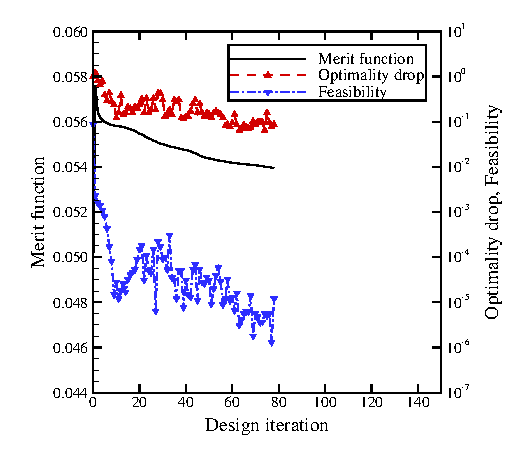
\includegraphics[width=4.5in]{Figures/With_Twist/CRM/optimize_CRM.eps}
\caption{Convergence history for NASA-CRM optimization with an upper sweep angle limit of 45.9\degree.}
\label{fig:crm_converge_45.9_Deg}
\end{figure}
Despite insufficient convergence, it was clear that this geometry had a very strong tendency to increase the wing sweep even further, as evidenced by the active wing sweep constraint very early on in the optimization. Performance had also greatly increased when compared to a baseline flow solution for the same geometry, which was trimmed to an angle of attack that would satisfy the lift constraint of $C_L S=1.6972$, as seen in Table~\ref{tab:crm_results}. The drag coefficient $C_D S$ had decreased by 50.5 drag counts with a small decrease in angle of attack. The $L/D$ had also increased by over 2.5 from 28.78 to 31.48. This substantial improvement in efficiency motivated the decision to halt the optimization and completely restart it with an increased sweep angle limit, as better performing optima may be located at higher sweep angles.


\begin{table}[!tp]
\centering
\caption{Results summary for the optimization of the NASA CRM}
\label{tab:crm_results}
\begin{adjustbox}{center}
\begin{tabular}{lcccc}
\hline\hline
Design Variable & Trimmed Baseline & 45.9\degree\ Sweep Limit & 50.0\degree\ Sweep Limit & 60.0\degree\ Sweep Limit\\
\hline
$S$ (ref. units\textsuperscript{2}) & 3.395 & 3.388 & 3.385 & 3.384 \\
$C_L S$ & 1.6972 & 1.6972 & 1.6972 & 1.6972 \\
$C_M S$ & -2.704 & -3.439 & -3.837 & -3.842 \\
$C_D S$ (counts) & 589.7 & 539.2 & 529.4 & 528.8 \\
$L/D$ & 28.78 & 31.48 & 32.06 & 32.08 \\
Angle of Attack & 1.982\degree\ & 1.436\degree\ & 0.909\degree\ & 0.848\degree\ \\
\makecell[l]{Post-Optimization\\Leading Edge Sweep Angle} & 37.50\degree\ & 45.77\degree\ & 49.16\degree\ & 49.05\degree\ \\
\hline\hline
\end{tabular}
\end{adjustbox}
\end{table}

The second case was run with a sweep angle limit expanded to 50\degree, which after converting to units of MAC and truncating, resulted in an increased upper sweep angle limit of 50.0\degree.
This case was run for over 200 iterations, with continual decreases in the merit function and feasibility observed, as seen in Figure~\ref{fig:crm_converge_50.0_Deg}. However, the optimality struggled to drop further than $10^{-1}$ below its original value.

Analysis of the optimization iteration history illustrated that the optimized geometry possesses a sweep angle very close to the sweep angle limit of 50.0\degree. The sweep angle had increased to 49.16\degree, with further improvements in $C_D S$ by 9.8 drag counts over the 45.9\degree\ sweep limit case. Meanwhile, the angle of attack decreased by over 0.5\degree, dropping from 1.436\degree\ to 0.909\degree. When converted to units of MAC, the margin between the optimized sweep angle and the upper sweep angle limit was just 0.131 reference units. This value is only 8\% of the 50.0\degree\ sweep angle limit of 1.600 reference units. Given this small margin, the continued performance improvements at higher sweep angles, and the strong decrease observed in the feasibility past 200 design iterations in Figure~\ref{fig:crm_converge_50.0_Deg}, it was decided that the sweep angle should be increased further as there may yet be better performance to be obtained.

\begin{figure}[!tp]
\centering
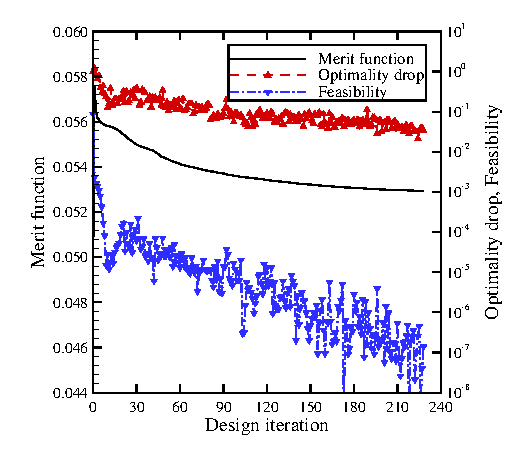
\includegraphics[width=4.5in]{Figures/With_Twist/CRM/Optimize_CRM_50deg.eps}
\caption{Convergence history for NASA-CRM optimization with an upper sweep angle limit of 50.0\degree.}
\label{fig:crm_converge_50.0_Deg}
\end{figure}

The last CRM case to be run made use of the last optimized geometry from the 50.0\degree\ sweep angle limit case as its initial geometry. The upper sweep angle limit was expanded further to 60.0\degree. This case was run for 60 iterations and observed no substantial changes to the merit function and optimality, whereas the feasibility decreased by one order of magnitude to approximately $10^{-8}$, as seen in Figure~\ref{fig:crm_converge_60.0_Deg}.

\begin{figure}[!tp]
\centering
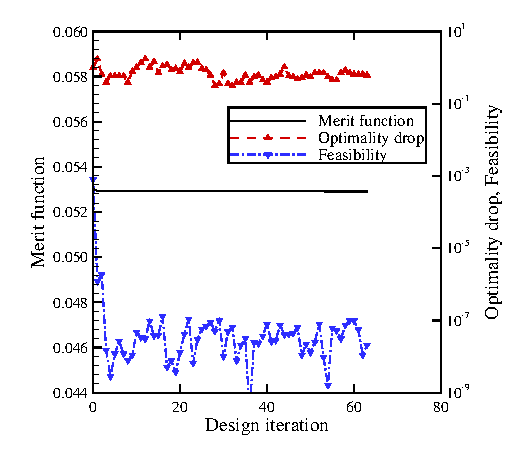
\includegraphics[width=4.5in]{Figures/With_Twist/CRM/Optimize_CRM_60deg.eps}
\caption{Convergence history for NASA-CRM optimization with an upper sweep angle limit of 60.0\degree.}
\label{fig:crm_converge_60.0_Deg}
\end{figure}
Performance for this geometry did not change significantly compared to the 50.0\degree\ sweep angle limit case. The $C_D S$ decreased by 0.6 drag counts to 528.8, the $L/D$ increased by 0.02 to 32.08, and the angle of attack decreased by 0.061\degree\ to 0.848\degree, as seen in Table~\ref{tab:crm_results}. Notably, the sweep angle decreased from the 50.0\degree\ case's most optimal point, dropping 0.1\degree\ from 49.16\degree\ to 49.05\degree, indicating further convergence towards the optimum obtained in the 50.0\degree sweep limit case.

Plots of the upper surface pressure contours for the 60.0\degree\ sweep angle limit optimized planform and the baseline flow solution—trimmed to an angle of attack that satisfies the lift constraint (trimmed angle of attack baseline)—are shown in Figure~\ref{fig:crm_planform_plots}. Plots of the section geometry and pressure distribution at various spanwise sections for the 60.0\degree\ sweep angle limit optimized planform and the trimmed angle of attack baseline are shown in Figure~\ref{fig:crm_section_plots}.

\begin{figure}[!tp]
    \centering
    \subfloat[\label{fig:crm_baseline_planform}]{\includegraphics[trim={0.25cm 0.25cm 0.25cm 0.25cm},clip,width=3.175in]{Figures/With_Twist/CRM/NASA_CRM_Baseline_Trimmed-Contour-Upper.eps}}
    \hspace{0.25cm}
    \subfloat[\label{fig:crm_60_deg_planform}]{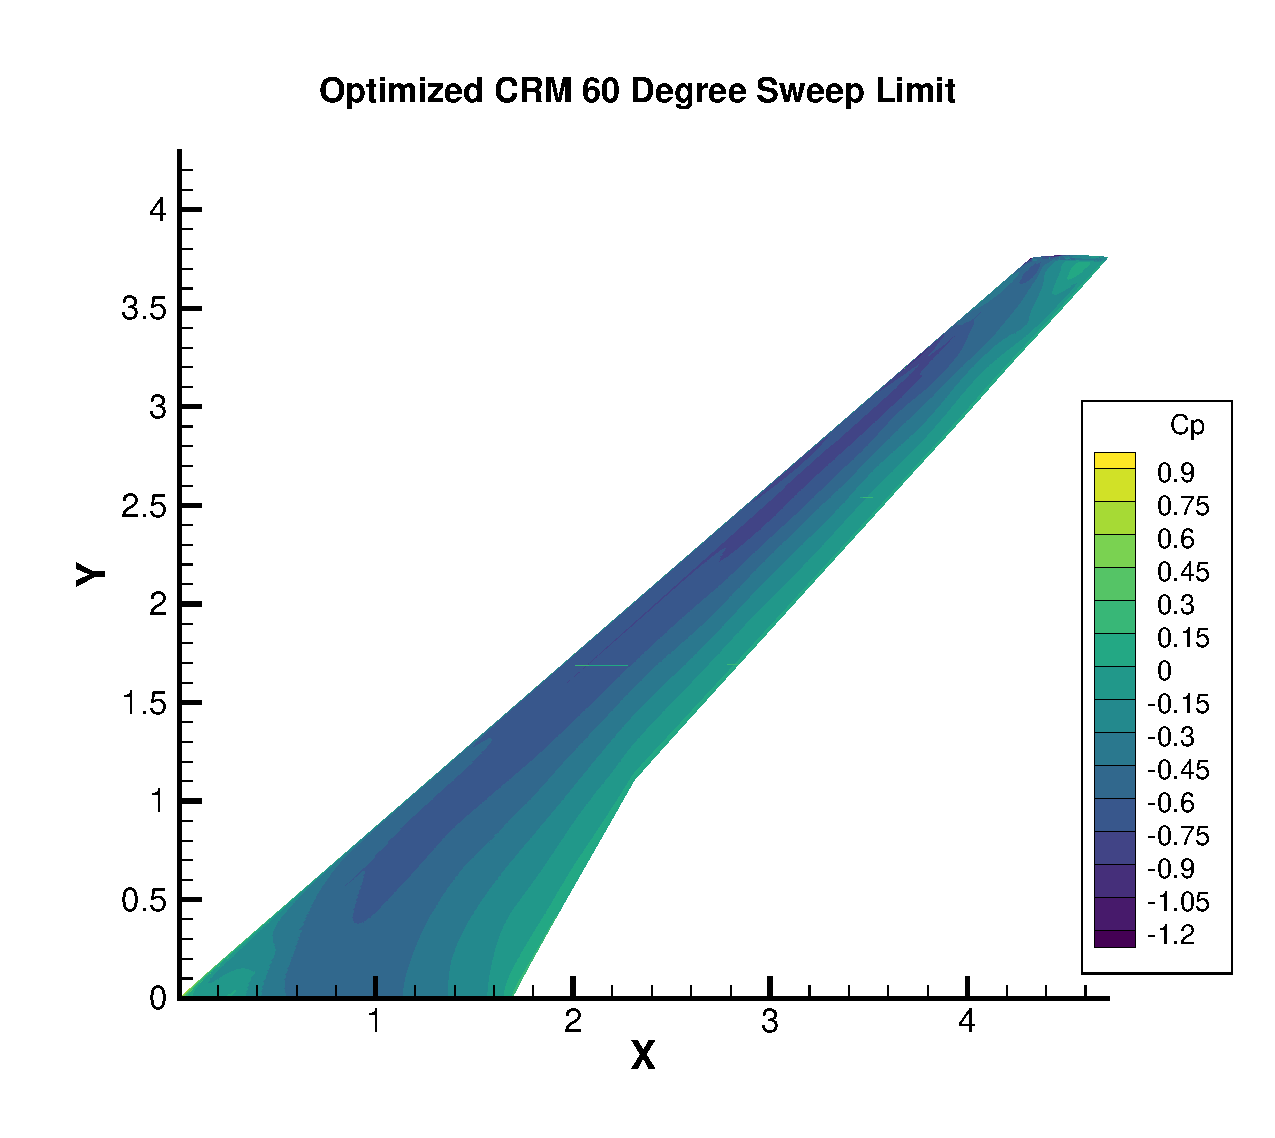
\includegraphics[trim={0.25cm 0.25cm 0.25cm 0.25cm},clip,width=3.175in]{Figures/With_Twist/CRM/NASA_CRM_varsweep_60deg-Contour-Upper.eps}}
    \caption{Upper surface pressure contours for the trimmed angle of attack baseline planform (\ref{fig:crm_baseline_planform}) and the 60.0\degree\ sweep angle limit optimized planform (\ref{fig:crm_60_deg_planform}).}
\label{fig:crm_planform_plots}
\end{figure}

\begin{figure}[!tp]
    \centering
    \subfloat[\label{fig:crm_section_1_perc}]{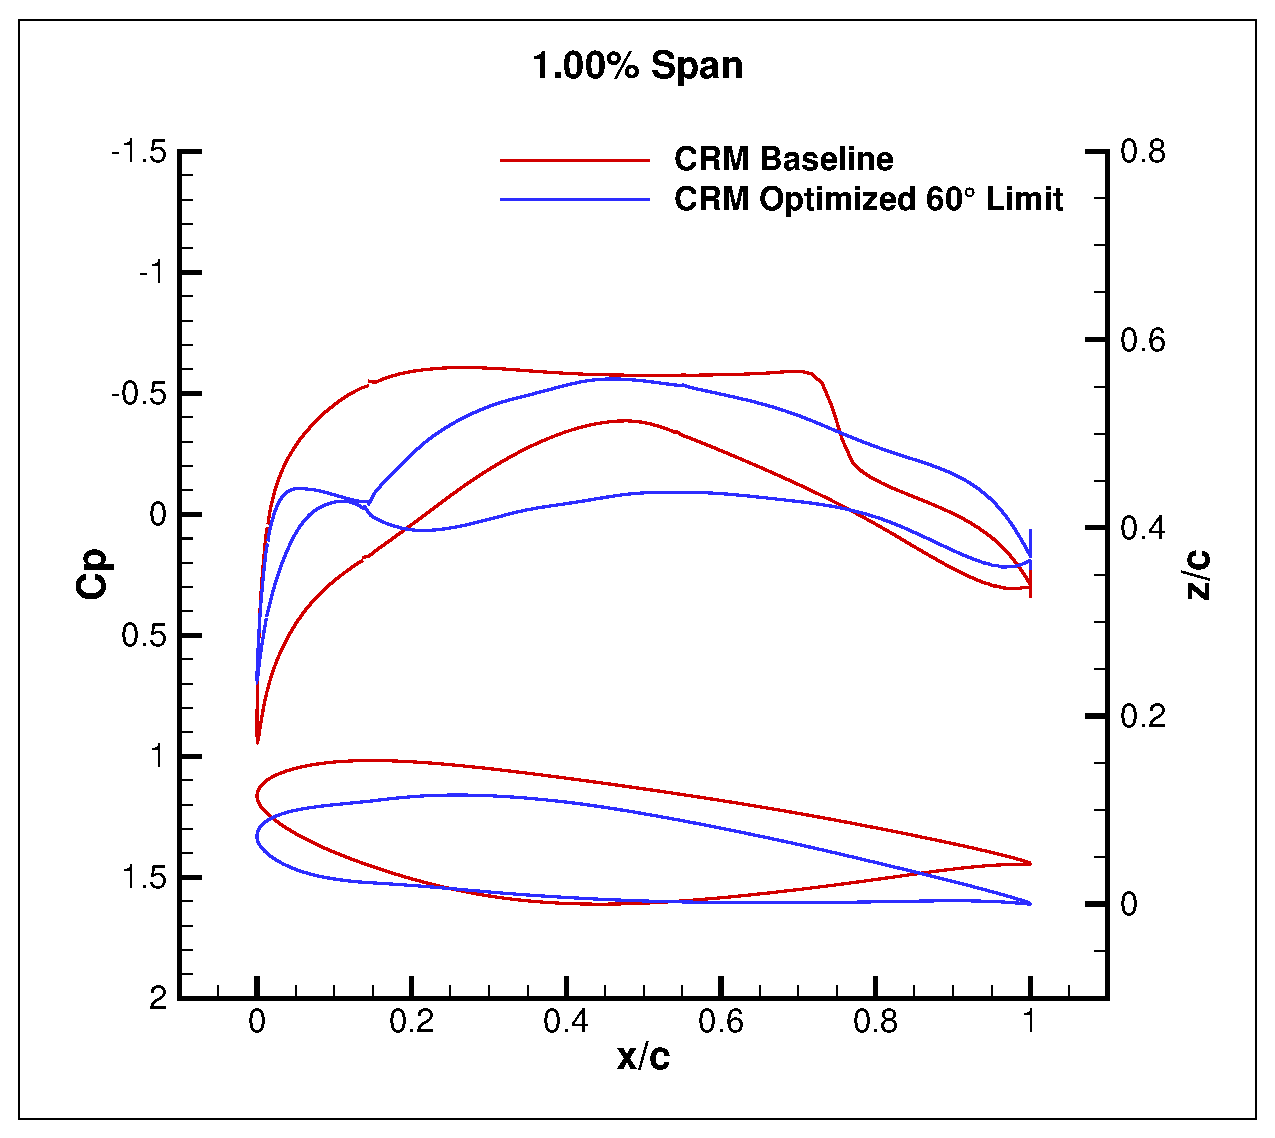
\includegraphics[trim={0.25cm 0.25cm 0.25cm 0.25cm},clip,width=3in]{Figures/With_Twist/CRM/NASA_CRM_Optimize_60deg-1percent_Span.eps}}
    \hspace{0.25cm}
    \subfloat[\label{fig:crm_section_20.6_perc}]{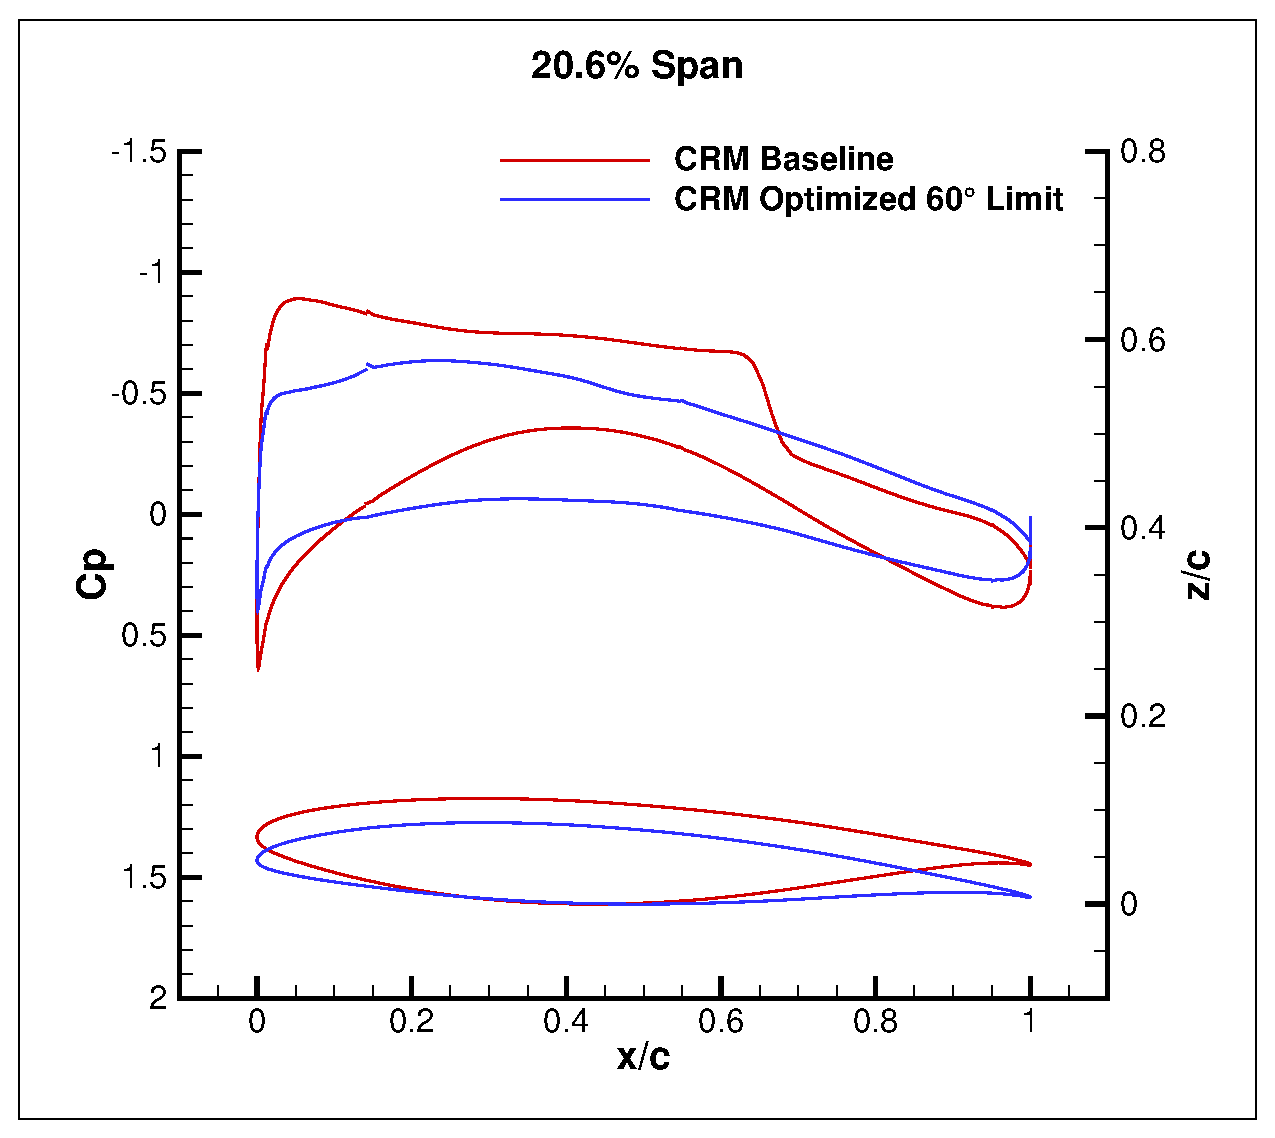
\includegraphics[trim={0.25cm 0.25cm 0.25cm 0.25cm},clip,width=3in]{Figures/With_Twist/CRM/NASA_CRM_Optimize_60deg-20.6percent_Span.eps}}\\
    \subfloat[\label{fig:crm_section_40.2_perc}]{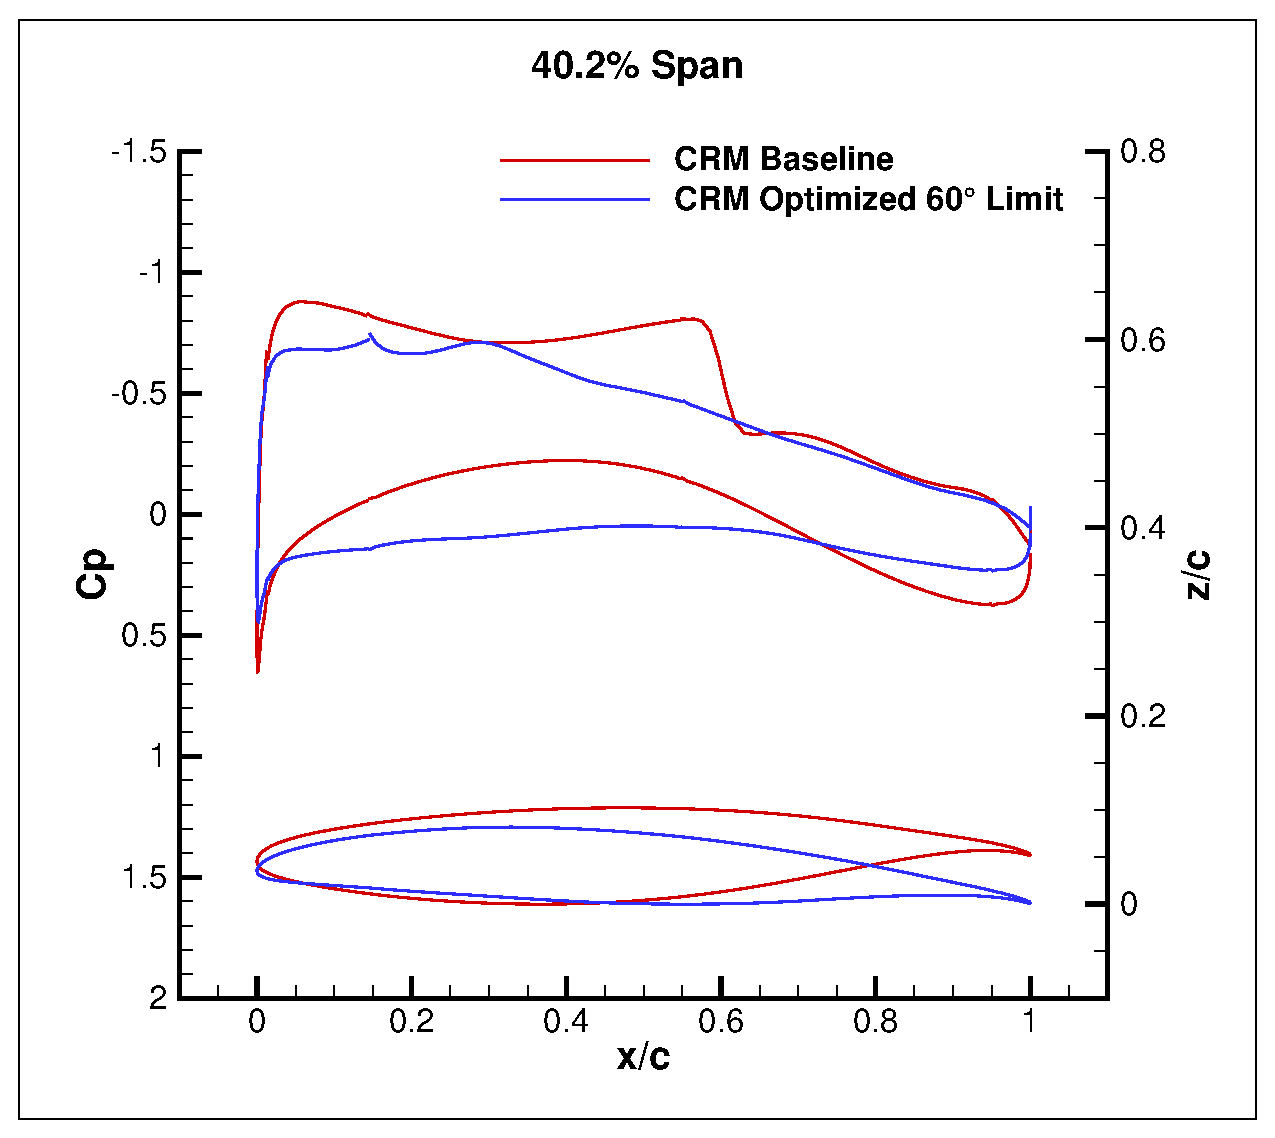
\includegraphics[trim={0.25cm 0.25cm 0.25cm 0.25cm},clip,width=3in]{Figures/With_Twist/CRM/NASA_CRM_Optimize_60deg-40.2percent_Span.eps}}
    \hspace{0.25cm}
    \subfloat[\label{fig:crm_section_59.8_perc}]{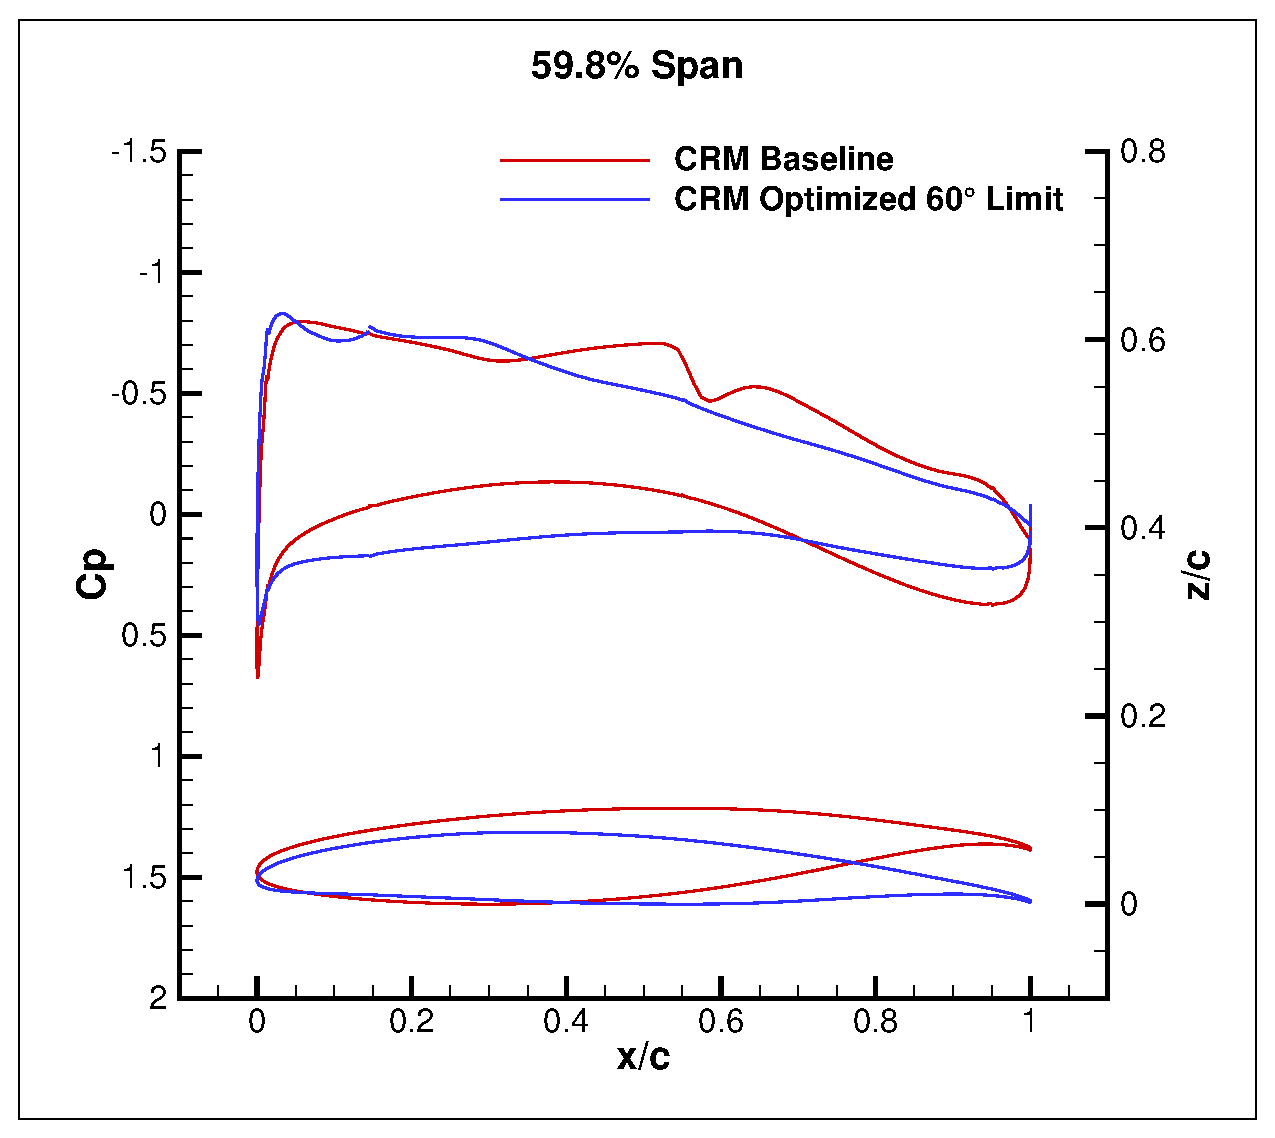
\includegraphics[trim={0.25cm 0.25cm 0.25cm 0.25cm},clip,width=3in]{Figures/With_Twist/CRM/NASA_CRM_Optimize_60deg-59.8percent_Span.eps}}\\
    \subfloat[\label{fig:crm_section_79.4_perc}]{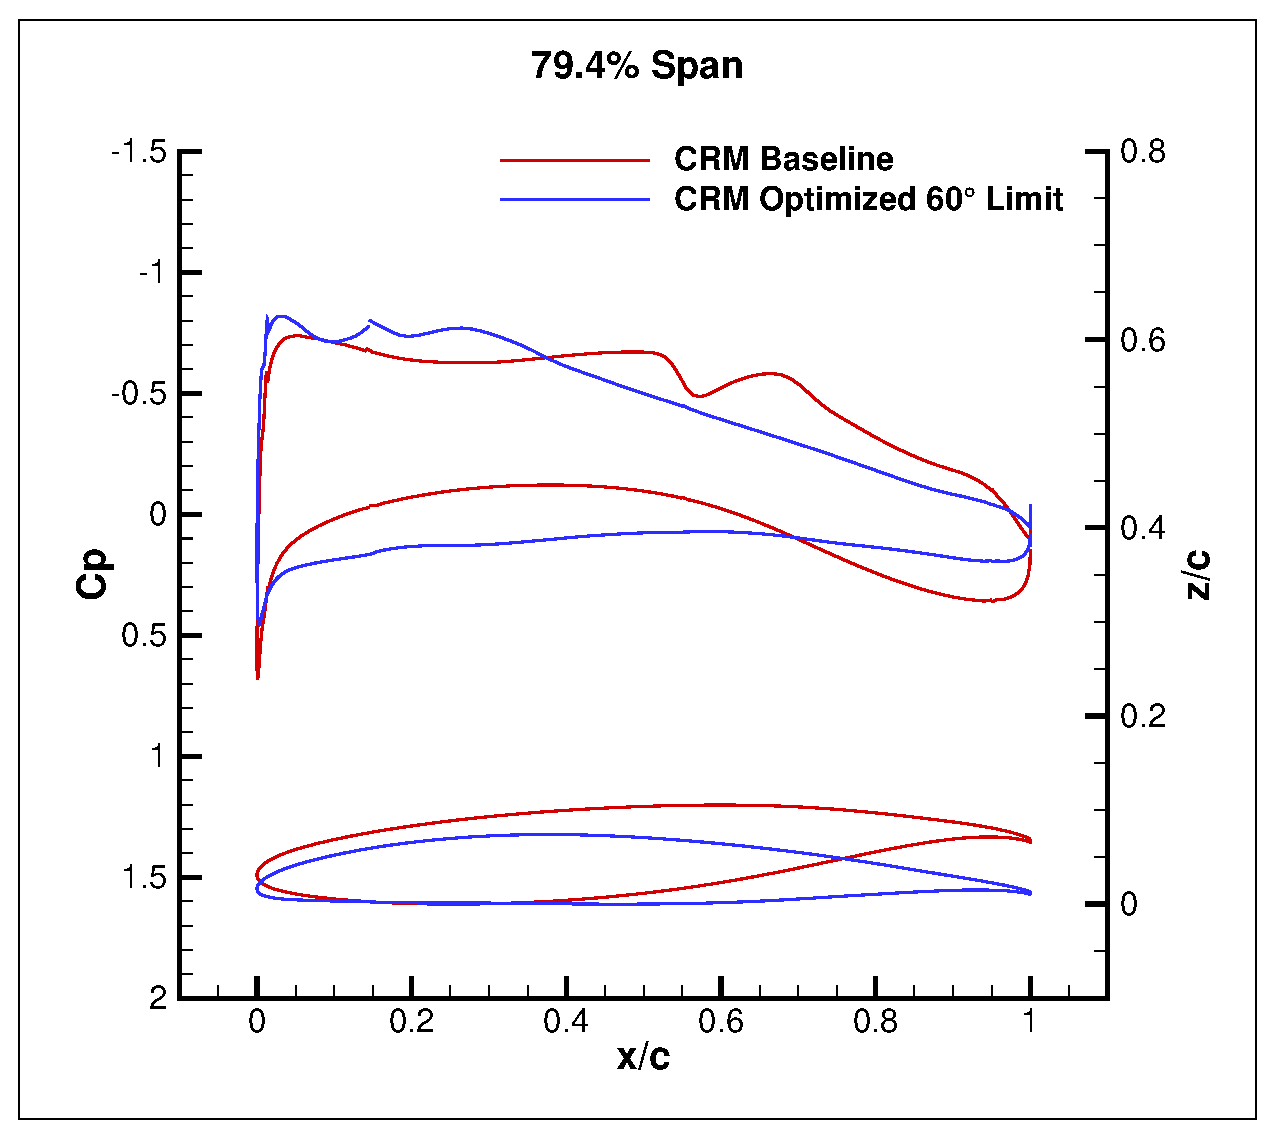
\includegraphics[trim={0.25cm 0.25cm 0.25cm 0.25cm},clip,width=3in]{Figures/With_Twist/CRM/NASA_CRM_Optimize_60deg-79.4percent_Span.eps}}
    \hspace{0.25cm}
    \subfloat[\label{fig:crm_section_99.0_perc}]{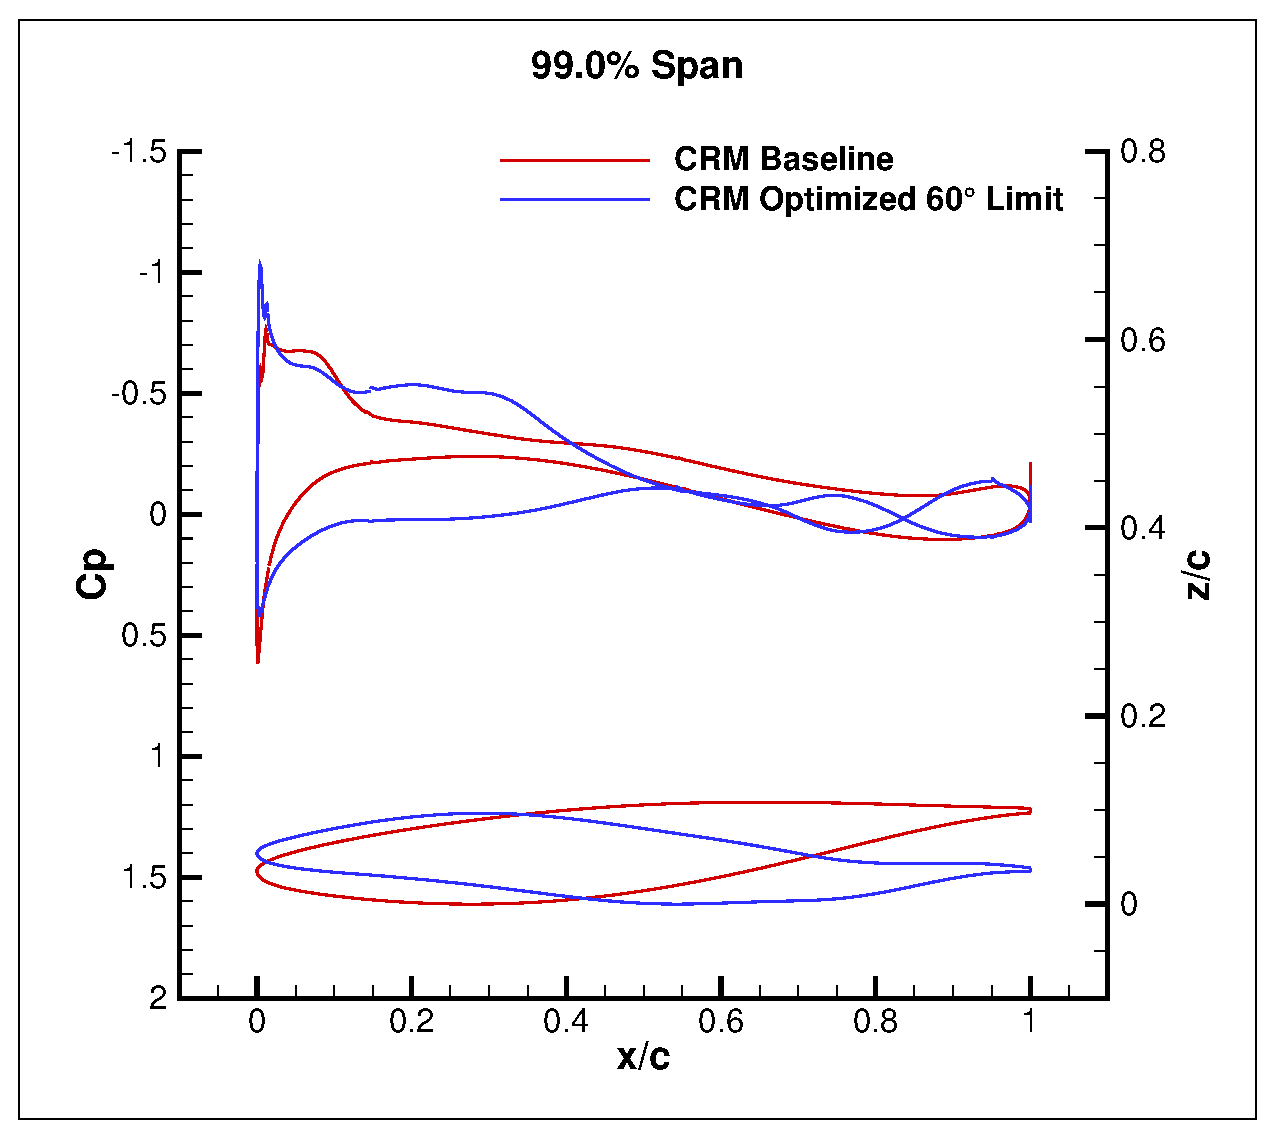
\includegraphics[trim={0.25cm 0.25cm 0.25cm 0.25cm},clip,width=3in]{Figures/With_Twist/CRM/NASA_CRM_Optimize_60deg-99.0percent_Span.eps}}
    \caption{Section geometry and pressure distribution plots of the trimmed angle of attack NASA CRM baseline planform and 60.0\degree\ sweep angle limit optimized planform at 1.00\% (\ref{fig:crm_section_1_perc}), 20.6\% (\ref{fig:crm_section_20.6_perc}), 40.2\% (\ref{fig:crm_section_40.2_perc}), 59.8\% (\ref{fig:crm_section_59.8_perc}), 79.4\%(\ref{fig:crm_section_79.4_perc}), and 99.0\% (\ref{fig:crm_section_99.0_perc}) span.}
\label{fig:crm_section_plots}
\end{figure}
\FloatBarrier

The original geometry exhibits a shock along the entire span of the wing, as evidenced by the close clustering of pressure contour lines towards the trailing edge in Figure~\ref{fig:crm_baseline_planform}, and the sharp drop in pressure that occurs between 60-80\% of the local chord on the upper surface of the wing in Figure~\ref{fig:crm_section_plots}. The optimized geometry resulting from the 60.0\degree\ sweep angle limit is able to completely remove this shock. Furthermore, with the exception of the root and wingtip, the optimizer is able to produce a smooth pressure recovery over the wing, as seen in Figures~\ref{fig:crm_section_20.6_perc}-\ref{fig:crm_section_79.4_perc}. This is also seen in the planform contour plot in Figure~\ref{fig:crm_60_deg_planform}, where the optimized planform displays a more equal spacing between contour lines compared to the trimmed baseline contour plot.

The section shape of the optimized wing differs dramatically from the baseline geometry. The thickness is reduced along the entire span, which differs from other studies. However, this is expected as the CRM optimization case defined in this study does not include a volume constraint, which is contrary to the definitions outlined by the ADODG case. Such a constraint would require the optimizer to redistribute the wing volume to the root~\cite{koo_investigation_2018}. The negative camber towards the root of the wing is reduced in magnitude, with the section becoming increasingly symmetric. Meanwhile, the camber is reduced from 20.6\% span and outboard, with the exception of the wingtip. Furthermore, the negative wing twist is reduced from mid-span and outboard. These camber and wing twist results disagree with the results obtained by by Koo and Zingg~\cite{koo_investigation_2018}, but agree with the results obtained by Lyu et al. and Kenway et al.~\cite{lyu_aerodynamic_2015, kenway_multipoint_2015}—although all three made use of a volume constraint. 
Strange behaviour occurs towards the wingtip. As seen in Figure~\ref{fig:crm_section_99.0_perc}, the leading half of the wing exhibits a negative twist, whereas the trailing half of the wing appears to be at a similar twist relative to the section at 79.4\% span in Figure~\ref{fig:crm_section_79.4_perc}. The overall twist at 99.0\% span appears to be a substantial reduction compared to the original geometry, but it is unclear why this result has occurred. This behaviour is unique to this study and does not appear in previous aerodynamic shape optimizations on the NASA CRM wing~\cite{koo_investigation_2018, shi-dong_adjoint-based_2017, lyu_aerodynamic_2015, kenway_multipoint_2015}. It must be noted that the spanwise sections used for measurement in this study differ from those specified in ADODG Case 4 and reported in other studies~\cite{martins_aerodynamic_2022, koo_investigation_2018, shi-dong_adjoint-based_2017, lyu_aerodynamic_2015, kenway_multipoint_2015}, such that the root and wingtip sections measured in this study are not the same as those used in ADODG Case 4. The section measured closest to the root is at 1.00\% span in this study whereas ADODG Case 4 reports measurements at 2.35\%. Similarly, section closest to the wingtip in this study occurs at 99.0\% span, whereas the measurement is taken at 94.4\% span in ADODG Case 4.. It is possible that analysis of the sections using the spanwise points dictated by ADODG Case 4 may show that such artifacts do not occur at its outermost measurement section at 94.4\% span. Nevertheless, the overall increase in twist from 20.6\% span to the wingtip disagrees with the results obtained by Koo and Zingg~\cite{koo_investigation_2018}, but closely agrees with the results obtained by Lyu et al. and Kenway et al.~\cite{lyu_aerodynamic_2015, kenway_multipoint_2015}, with the exception of the section shape at the wingtip. All three studies present slight variations on ADODG case 4 with respect to their optimization constraints, such that all three studies produce slightly different results. Nevertheless, the changes in camber and thickness found in this study—with the exception of the root due to this study's exclusion of a volume constraint—otherwise match all three of the aforementioned studies' results.

%%%%%%%%%%%%%%%%%% TALK ABOUT WEIRD TWIST BEHAVIOUR HERE %%%%%%%%%%%%%%%%%%
The wing twist artifact occurring at 99.0\% span seen in Figure~\ref{fig:crm_section_99.0_perc} was of particular concern. Its varying twist along the chord does not agree with other studies, wherein such phenomena did not arise~\cite{koo_investigation_2018, lyu_aerodynamic_2015, kenway_multipoint_2015}. Analysis of the outboard sections of the 60.0\degree\ limit optimized geometry illustrated significant oscillations in wing twist, as seen in Figure~\ref{fig:crm_artifacts}. An additional optimization was conducted with a 45.0\degree\ upper sweep angle limit to observe if this behaviour occurs at lower sweep angles as well. Indeed, oscillations of similar magnitude occur at the trailing edge with a 45.0\degree sweep angle as well, as seen in Figure~\ref{fig:crm_artifacts_45deg}. This behaviour is not desirable, as it is not manufacturable within the context of conventional aircraft design. Therefore, an additional study was run on the NASA CRM with an otherwise identical methodology, with the exception of wing twist as a design variable and the selection of sweep angle limits, which are outlined in the following section.
% Also include images
\begin{figure}[!tp]
    \centering
    \subfloat[\label{fig:crm_artifact_01}]{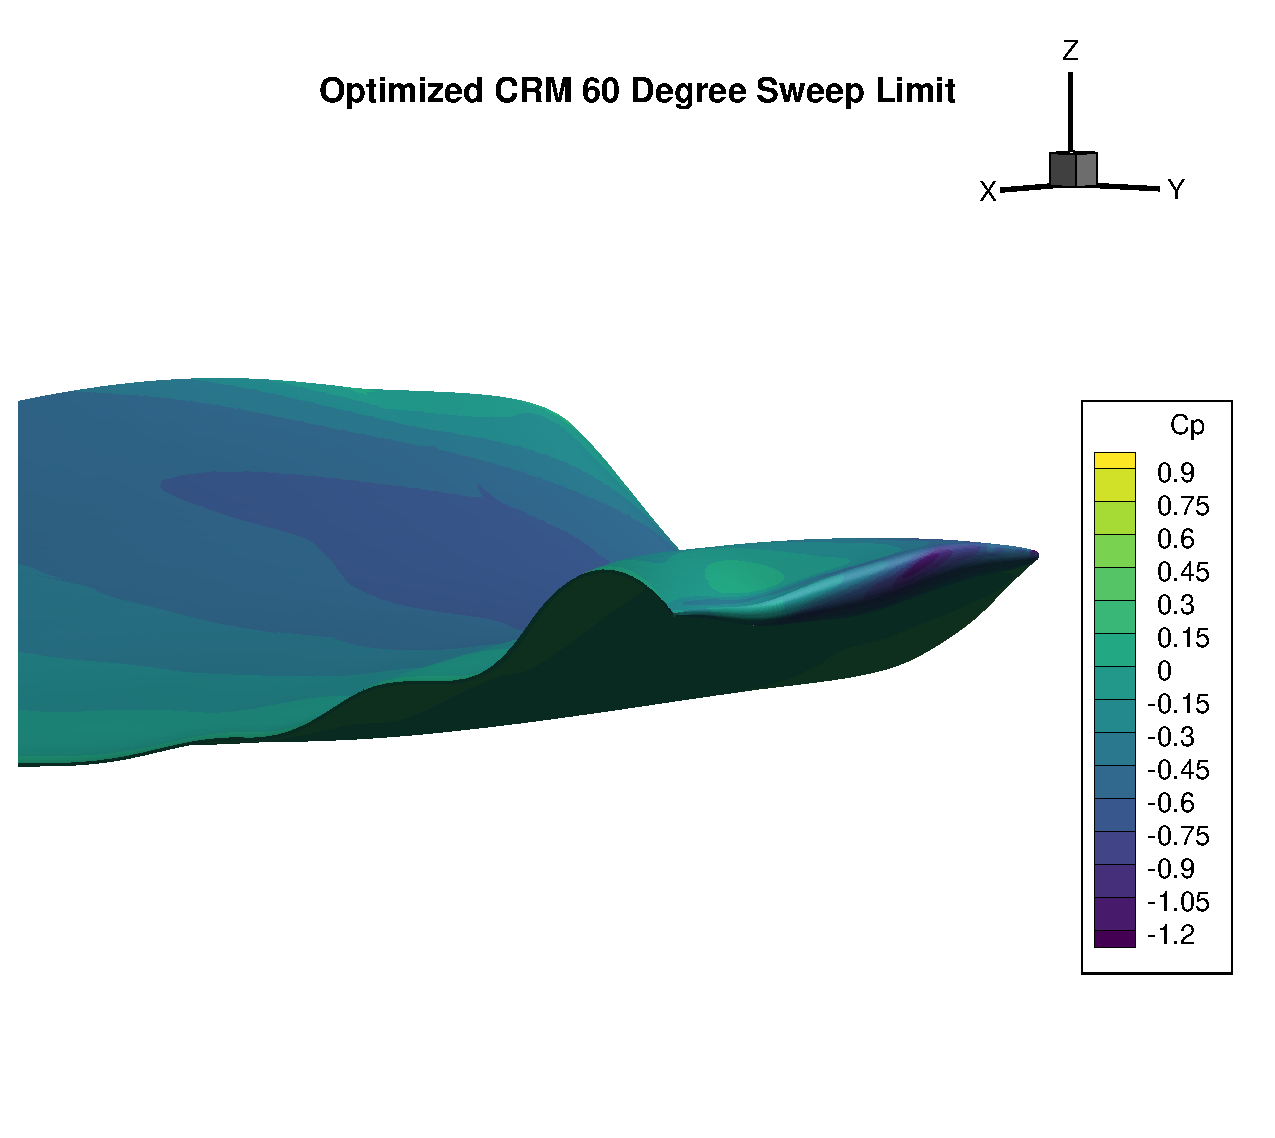
\includegraphics[trim={0.25cm 0.25cm 0.25cm 0.25cm},clip,width=3.175in]{Figures/With_Twist/CRM/Optimize_CRM_60deg_Twist_Artifact_01.eps}}
    \hspace{0.25cm}
    \subfloat[\label{fig:crm_artifact_02}]{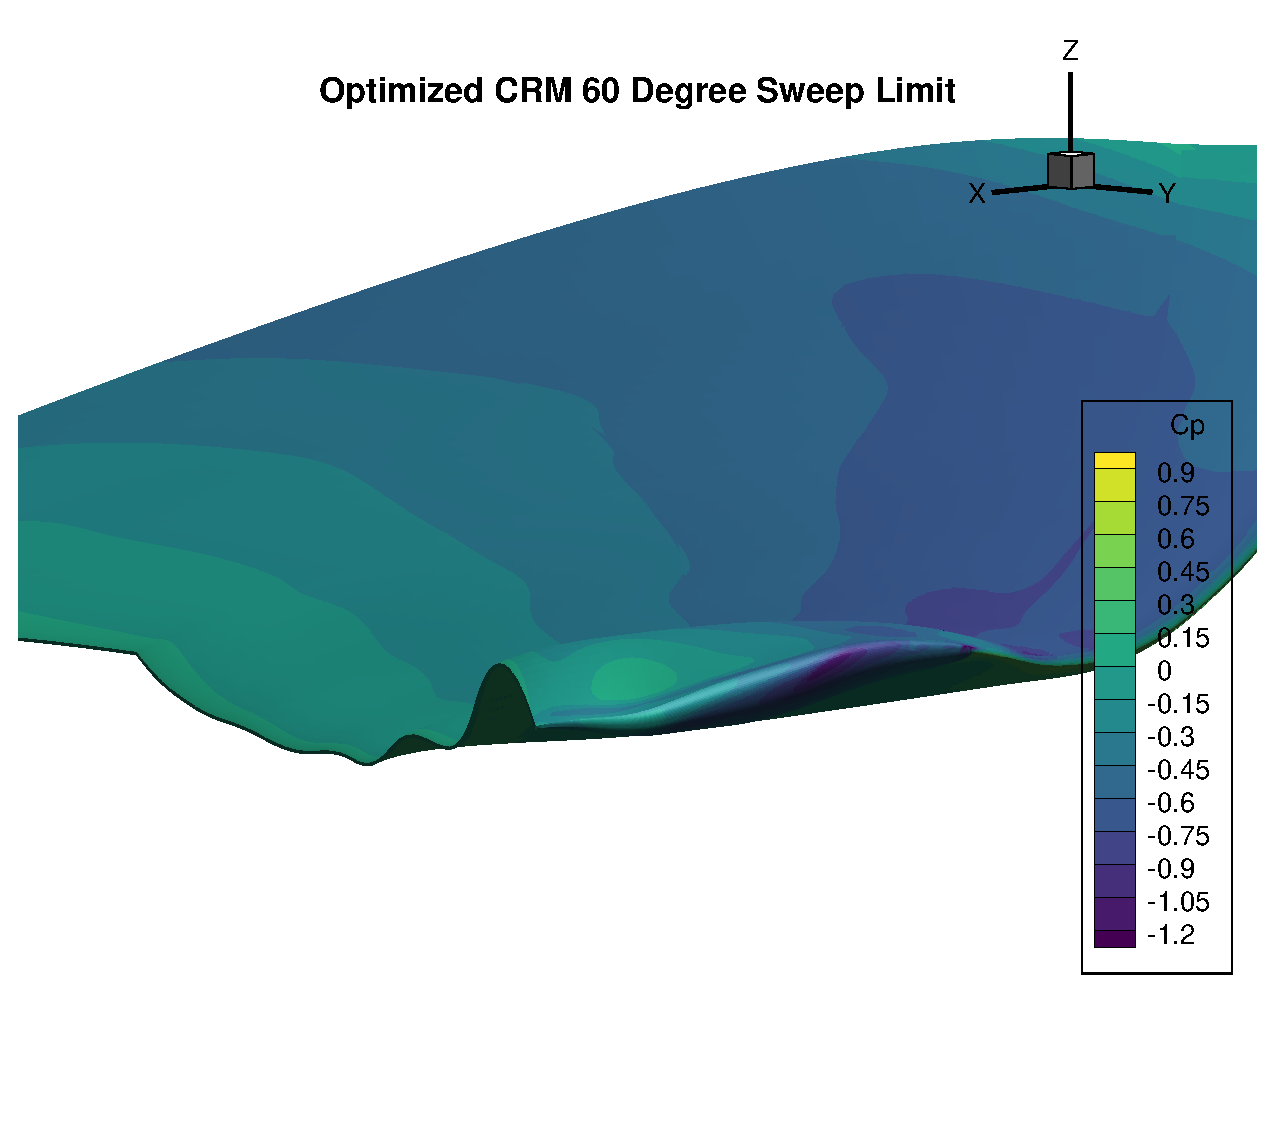
\includegraphics[trim={0.25cm 0.25cm 0.25cm 0.25cm},clip,width=3.175in]{Figures/With_Twist/CRM/Optimize_CRM_60deg_Twist_Artifact_02.eps}}
    \caption{Trailing edge geometry artifacts observed in the CRM 60.0\degree\ sweep angle limit optimized planform.}
\label{fig:crm_artifacts}
\end{figure}

\begin{figure}[!tp]
\centering
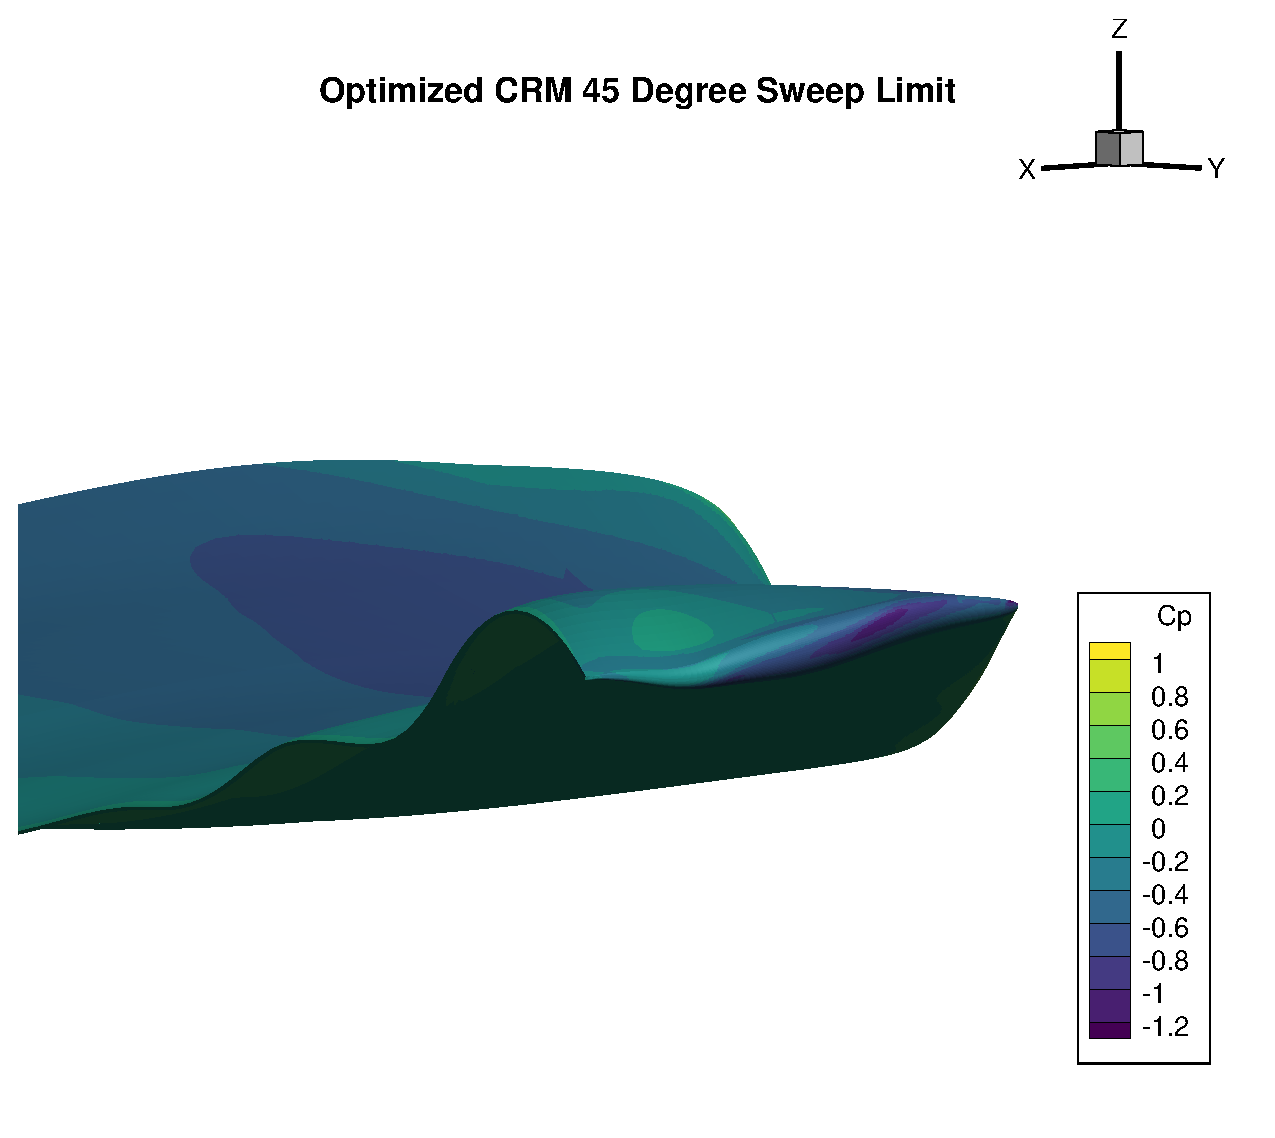
\includegraphics[width=4.5in]{Figures/With_Twist/CRM/Optimize_CRM_45deg_Twist_Artifact_01.eps}
\caption{Trailing edge geometry artifacts observed in a CRM 45.0\degree\ sweep angle limit optimized planform.}
\label{fig:crm_artifacts_45deg}
\end{figure}
%%%%%%%%%%%%%%%%%% INTRODUCE NEW CASE WITHOUT TWIST %%%%%%%%%%%%%%%%%%
\subsection{NASA CRM Optimization without Wing Twist}
\label{ssec:crm-opt-notwist}
In light of the geometry artifacts associated with wing twist on the NASA CRM wing, a second study was performed without wing twist as a design variable. The second case was run with an equality constraint on the wing twist set to 0\degree. Owing to the knowledge of optimization behaviour obtained in the initial CRM ASO study, the sweep angle was immediately expanded to 60.0\degree.

Furthermore, considering the substantial drag improvements obtained in the initial study on the CRM, ASO without wing twist was conducted on the NASA CRM at its original sweep angle of 37.5\degree\ as well. This result served to place the 60.0\degree\ sweep angle limit result without wing twist into context, as an optimization of the CRM at the original wing sweep angle is likely to be a more common method of optimizing a wing, as evidenced by many modern ASO studies~\cite{lyu_rans-based_2014, lyu_aerodynamic_2015, osusky_drag_2015, streuber_investigation_2017, koo_investigation_2018}. Therefore, the result obtained from this optimization was considered to be the benchmark over which the sweep-inclusive optimization must display a tangible benefit in order to be valuable.

%%%%%%%%% CRM WITHOUT TWIST RESULTS %%%%%%%%%%%
The CRM ASO with a fixed sweep angle matching the original sweep angle of 37.5\degree\ progressed very smoothly, with analysis of the merit function, optimality, and feasibility of this study illustrating that this case was converged after 267 design iterations, as seen in Figure~\ref{fig:crm_notwist_converge_optimized_baseline}. The drag coefficient $C_D S$ had decreased by 52.7 drag counts, with a small decrease in angle of attack, as seen in Table~\ref{tab:crm_notwist_results}. The $L/D$ increased by over 2.8 from 28.78 to 31.59. This performance is slightly better than that that obtained in the 45.9\degree\ case with wing twist in the initial study, but it must be noted that this case was not converged.

The CRM ASO with a sweep angle limit of 60.0\degree\ observed smooth convergence as well. Analysis of the merit function, optimality, and feasibility of this study indicated that this study had converged after 259 design iterations, as seen in Figure~\ref{fig:crm_notwist_converge_60.0_deg}. The drag coefficient, $C_D S$, had decreased by 58.8 drag counts relative to the trimmed baseline wing, with a small decrease in angle of attack, as seen in Table~\ref{tab:crm_notwist_results}. The moment coefficient, $C_M S$, decreased substantially from -2.704 to -3.742. The $L/D$ increased by over 3.1 from 28.78 to 31.59. This performance is an improvement by 1.14\% over the optimized CRM at the original sweep angle of 37.5\degree; however, the 60.0\degree\ case with twist included remains 0.43\% better than the 60.0\degree\ case without twist, with lower drag by 2.3 drag counts. Nonetheless, its geometry artifacts prevent it from being a legitimate comparison due to the unrealistic manufacturing requirements that would result. Therefore, the results without wing twist serve as this study's primary basis for wing sweep performance comparisons on the NASA CRM wing.

Plots of the upper surface pressure contours on the optimized planforms for the ASOs at the original sweep angle of 37.5\degree\ and the 60.0\degree\ sweep angle limit cases are shown in Figure~\ref{fig:crm_notwist_planform_plots}. Plots of the section geometry and pressure distribution at various spanwise sections for the trimmed angle of attack baseline, the fixed-sweep ASO at the original sweep angle of 37.5\degree, and the 60.0\degree\ sweep angle limit ASO cases are given in Figure~\ref{fig:crm_notwist_section_plots}.

\begin{table}[!tp]
\centering
\caption{Results summary for the optimization of the NASA CRM without wing twist}
\label{tab:crm_notwist_results}
\begin{adjustbox}{center}
\begin{tabular}{lcccc}
\hline\hline
Design Variable & Trimmed Baseline & Original (37.5\degree)\ Sweep Limit & 60.0\degree\ Sweep Limit\\
\hline
$S$ (ref. units\textsuperscript{2}) & 3.395 & 3.394 & 3.393\\
$C_L S$ & 1.6972 & 1.6972 & 1.6972\\
$C_M S$ & -2.704 & -2.717 & -3.742 \\
$C_D S$ (counts) & 589.7 & 537.2 & 531.1\\
$L/D$ & 28.78 & 31.59 & 31.96\\
Angle of Attack & 1.982\degree\ & 1.771\degree\ & 2.225\degree\ \\
\makecell[l]{Post-Optimization\\Leading Edge Sweep Angle} & 37.50\degree\ & 37.31\degree\ & 48.50\degree\ \\
\hline\hline
\end{tabular}
\end{adjustbox}
\end{table}
% images
%%%%%%%%% CRM WITHOUT TWIST CONVERGENCE HISTORY %%%%%%%%%%%
\begin{figure}[!tp]
\centering
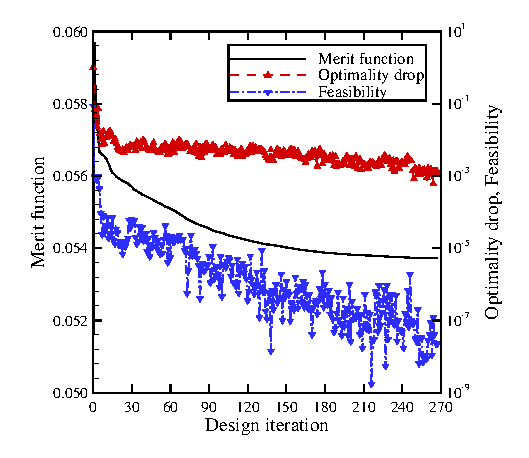
\includegraphics[width=4.5in]{Figures/No_Twist/NASA_CRM/Optimize_CRM_FIXED_Orig_No_Twist.eps}
\caption{Convergence history for NASA-CRM optimization without wing twist and a sweep angle limit at the original sweep angle of 37.5\degree.}
\label{fig:crm_notwist_converge_optimized_baseline}
\end{figure}

\begin{figure}[!tp]
\centering
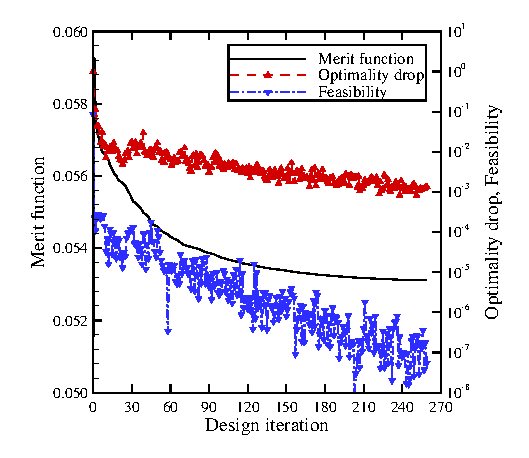
\includegraphics[width=4.5in]{Figures/No_Twist/NASA_CRM/Optimize_CRM_No_Twist_60deg.eps}
\caption{Convergence history for NASA-CRM optimization without wing twist and an upper sweep angle limit of 60.0\degree.}
\label{fig:crm_notwist_converge_60.0_deg}
\end{figure}

%%%%%%%%% CRM WITHOUT TWIST UPPER CP CONTOURS %%%%%%%%%%%
\begin{figure}[!tp]
    \centering
    %%%%%% Decided not to include original CRM again %%%%%%
    % \subfloat[\label{fig:crm_notwist_baseline_planform}]{\includegraphics[trim={0.25cm 0.25cm 0.25cm 0.25cm},clip,width=3.175in]{Figures/No_Twist/NASA_CRM/NASA_CRM_Baseline_Trimmed-Contour-Upper.eps}}\\
    \subfloat[\label{fig:crm_notwist_optimized_baseline_planform}]{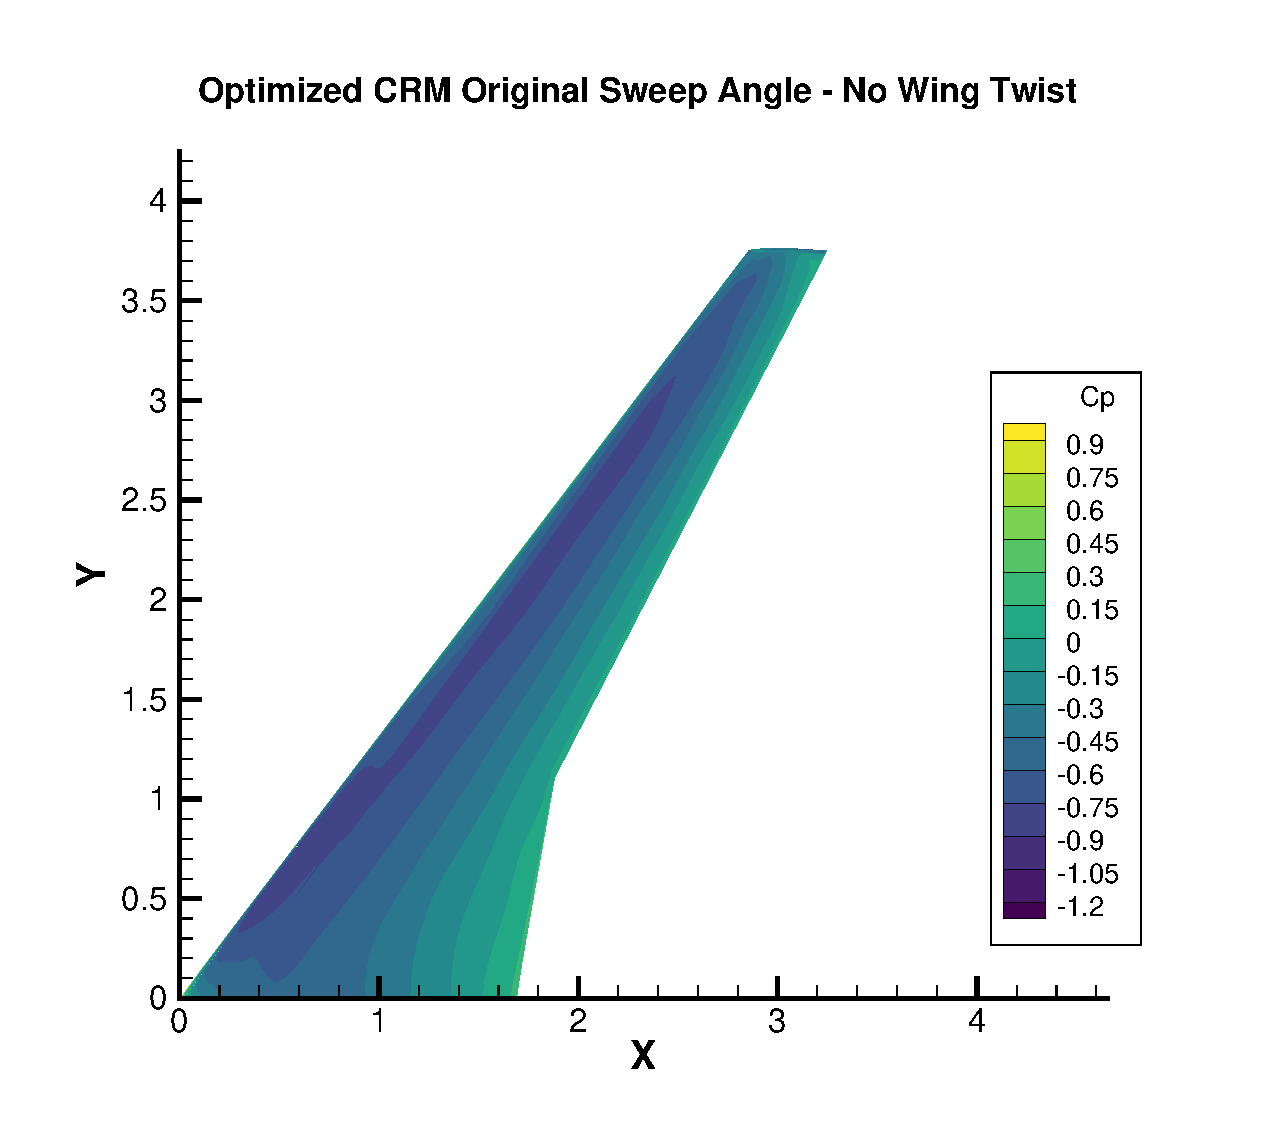
\includegraphics[trim={0.25cm 0.25cm 0.25cm 0.25cm},clip,width=3.175in]{Figures/No_Twist/NASA_CRM/NASA_CRM_FIXED_Orig_NoTwist-Contour-Upper.eps}}
    \hspace{0.25cm}
    \subfloat[\label{fig:crm_notwist_60_deg_planform}]{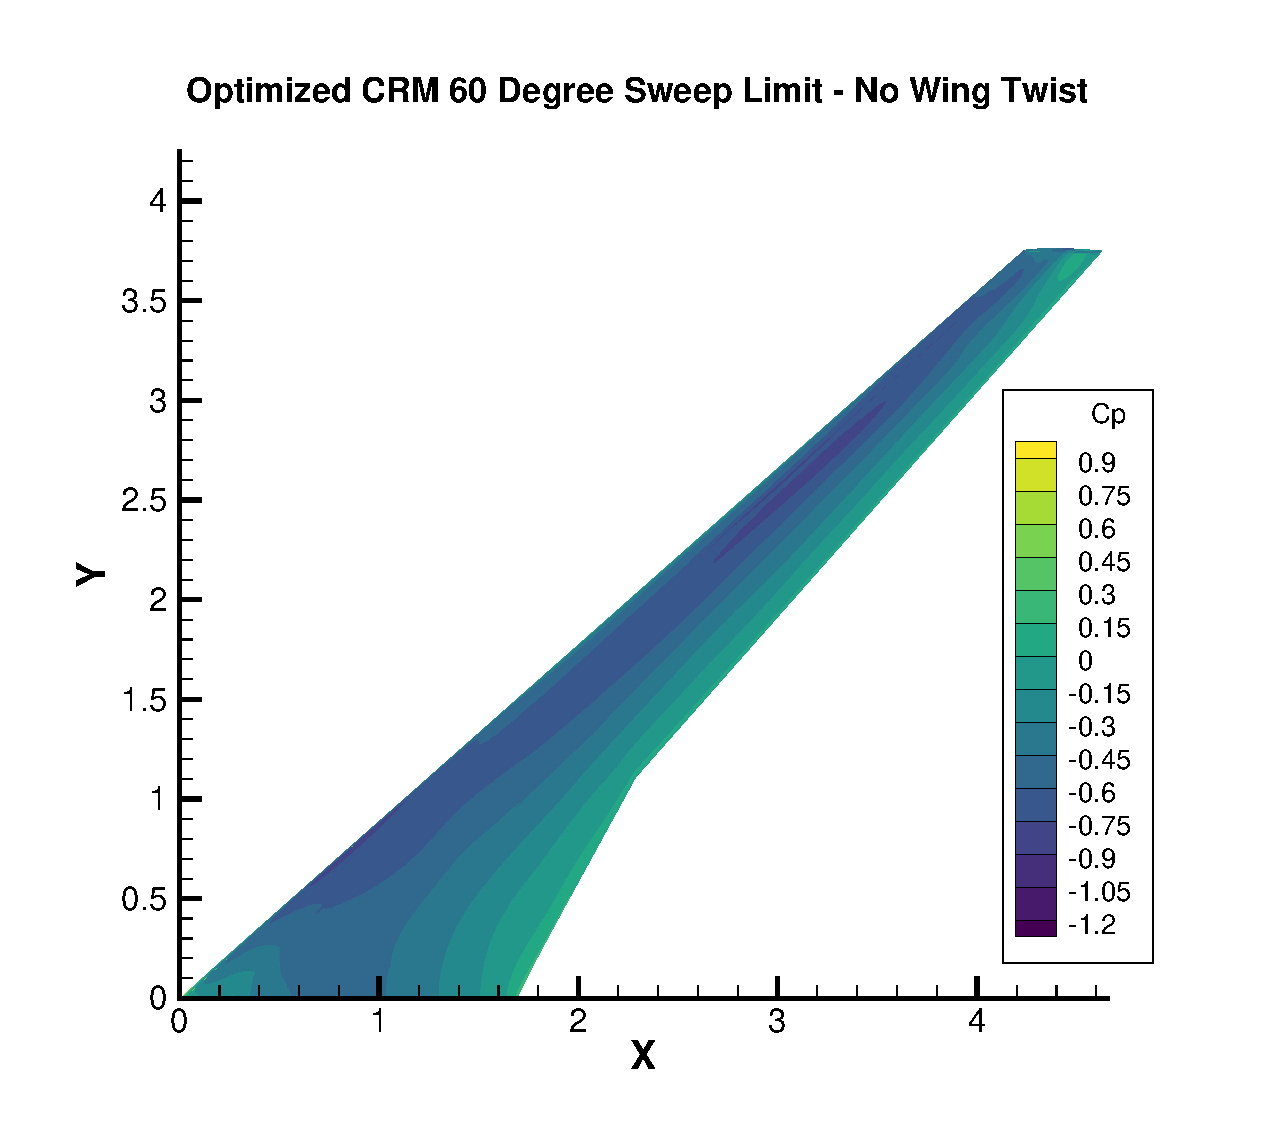
\includegraphics[trim={0.25cm 0.25cm 0.25cm 0.25cm},clip,width=3.175in]{Figures/No_Twist/NASA_CRM/NASA_CRM_varsweep_60deg_NoTwist-Contour-Upper.eps}}
    \caption{Upper surface pressure contours for the original sweep angle limit optimized planform (\ref{fig:crm_notwist_optimized_baseline_planform}) and the 60.0\degree\ sweep angle limit optimized planform (\ref{fig:crm_60_deg_planform}) without wing twist in optimization.}
\label{fig:crm_notwist_planform_plots}
\end{figure}

%%%%%%%%%% CRM WITHOUT TWIST SECTION SHAPES %%%%%%%%%%%
\begin{figure}[!tp]
    \centering
    \subfloat[\label{fig:crm_notwist_section_1_perc}]{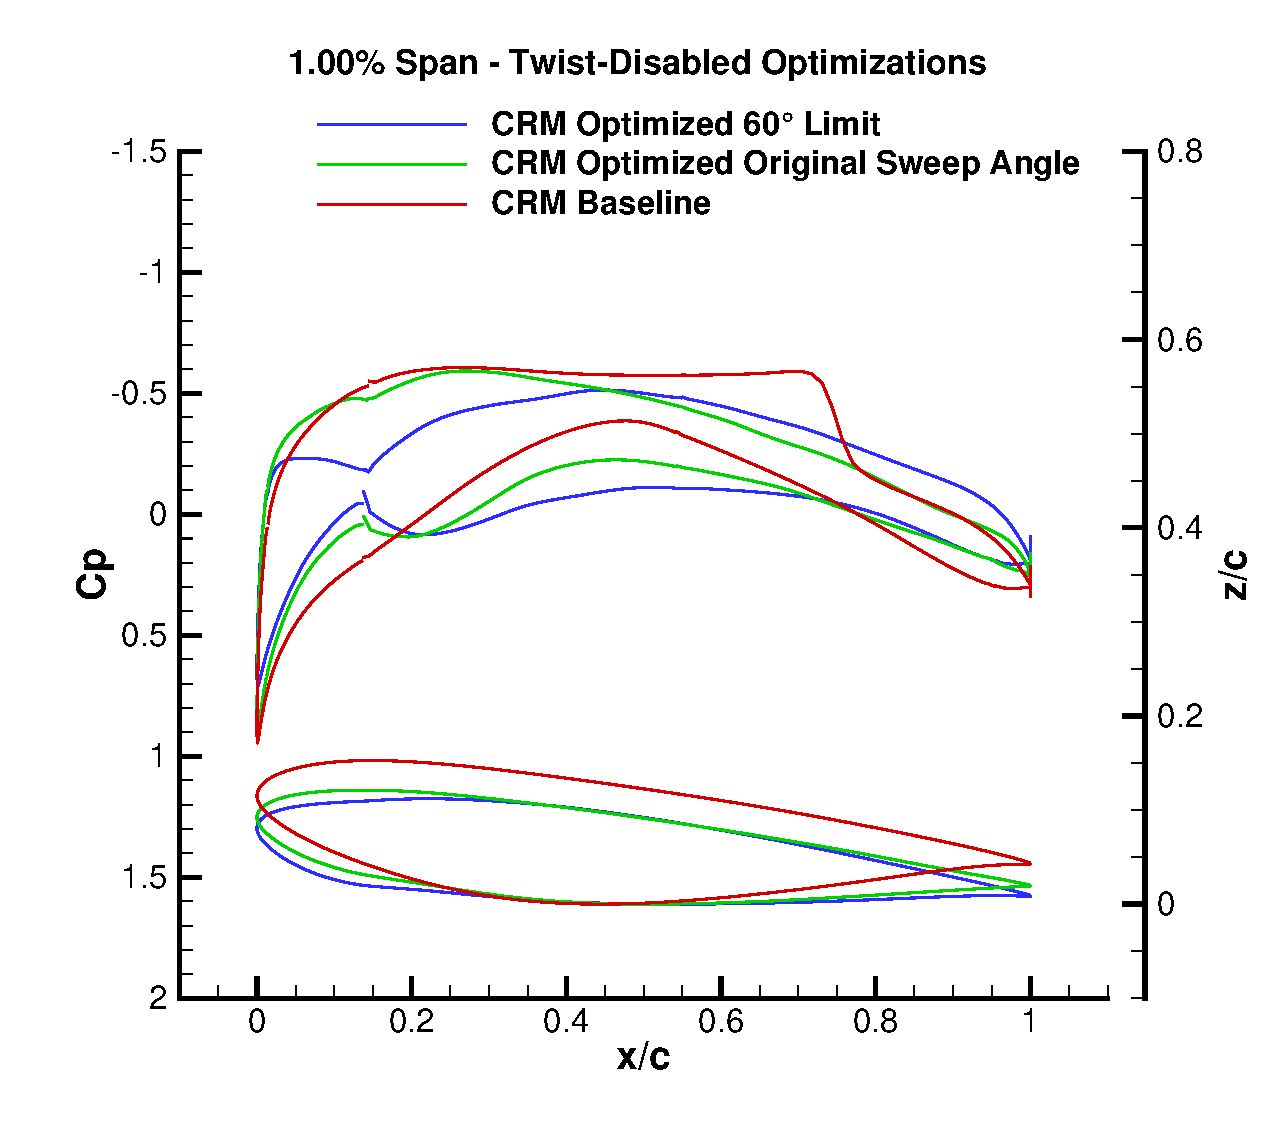
\includegraphics[trim={0.2cm 0.2cm 0.2cm 0.2cm},clip,width=3in]{Figures/No_Twist/NASA_CRM/NASA_CRM_Optimize_NoTwist-1.00percent_Span.eps}}
    \hspace{0.2cm}
    \subfloat[\label{fig:crm_notwist_section_20.6_perc}]{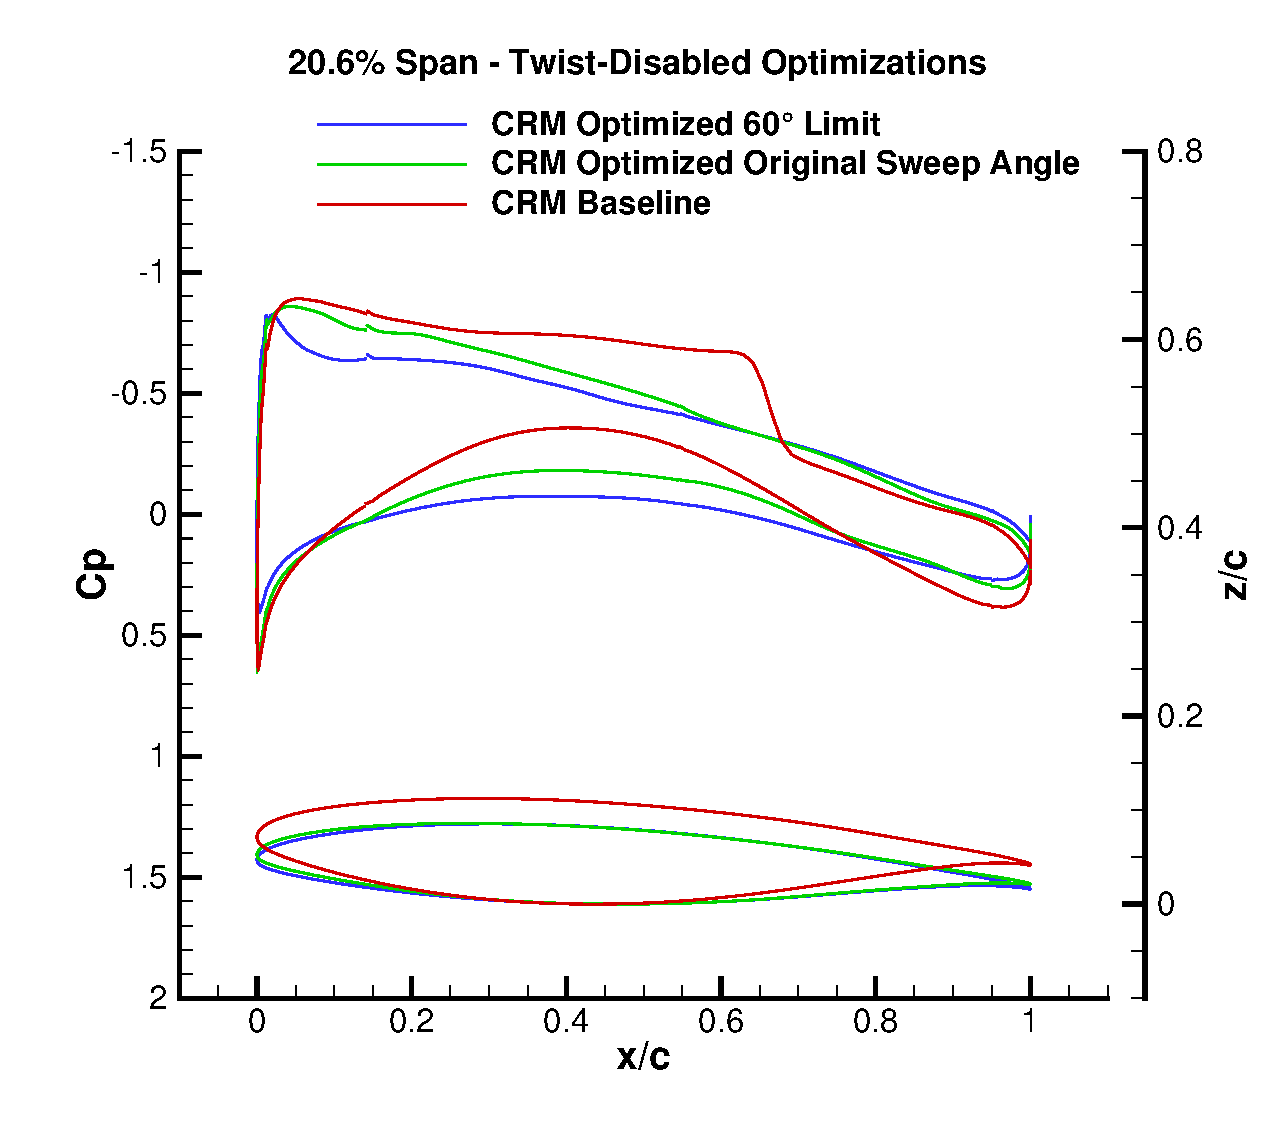
\includegraphics[trim={0.2cm 0.2cm 0.2cm 0.2cm},clip,width=3in]{Figures/No_Twist/NASA_CRM/NASA_CRM_Optimize_NoTwist-20.6percent_Span.eps}}\\
    \subfloat[\label{fig:crm_notwist_section_40.2_perc}]{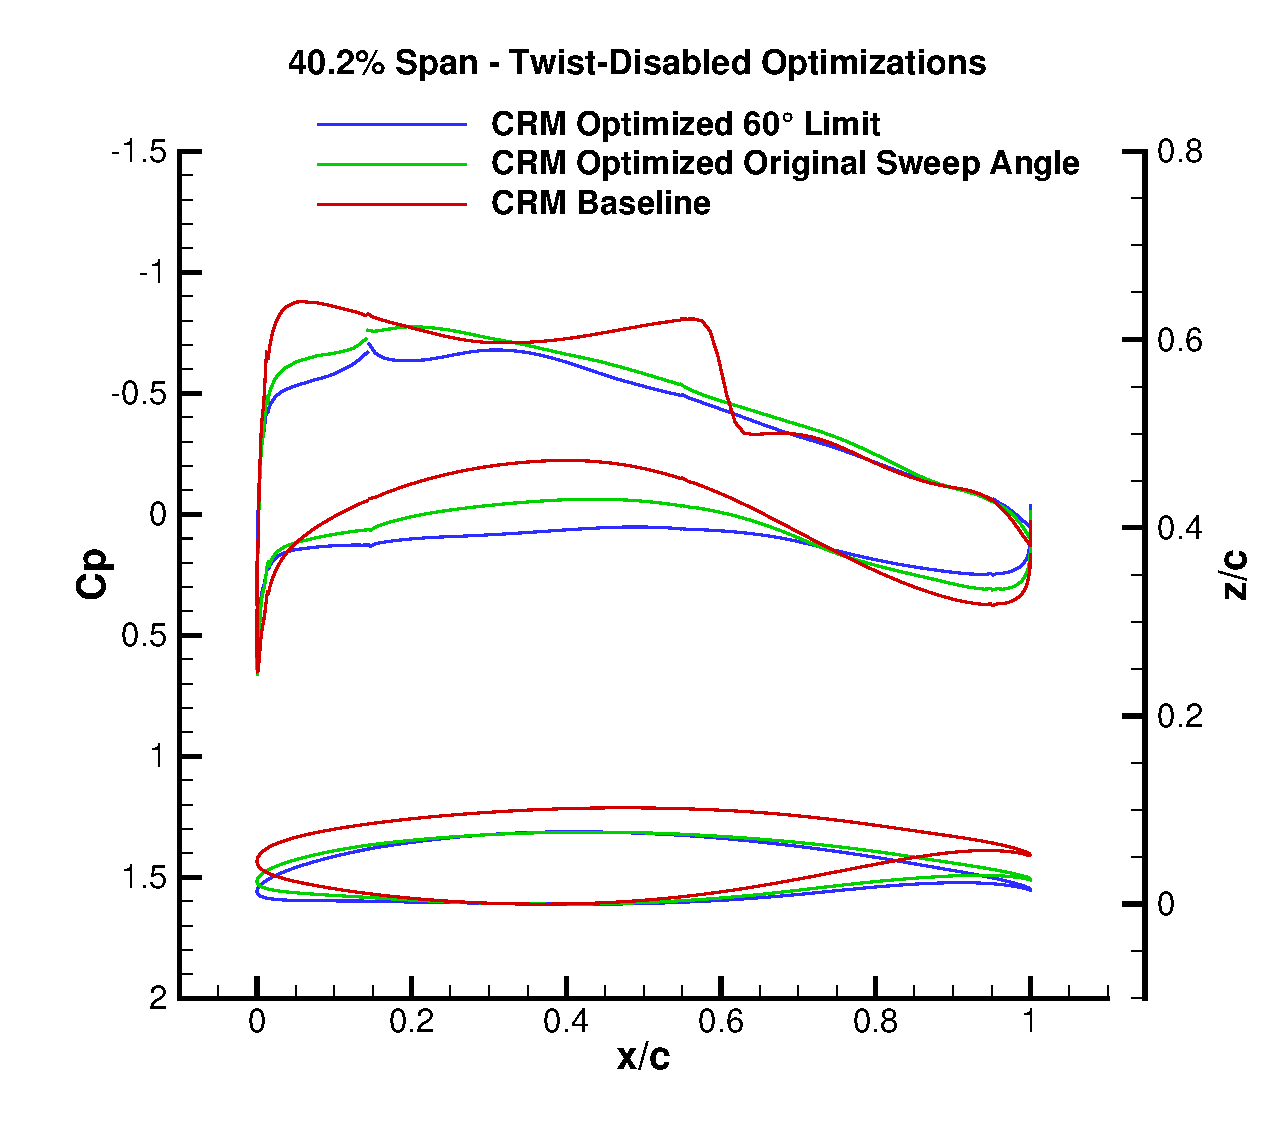
\includegraphics[trim={0.2cm 0.2cm 0.2cm 0.2cm},clip,width=3in]{Figures/No_Twist/NASA_CRM/NASA_CRM_Optimize_NoTwist-40.2percent_Span.eps}}
    \hspace{0.2cm}
    \subfloat[\label{fig:crm_notwist_section_59.8_perc}]{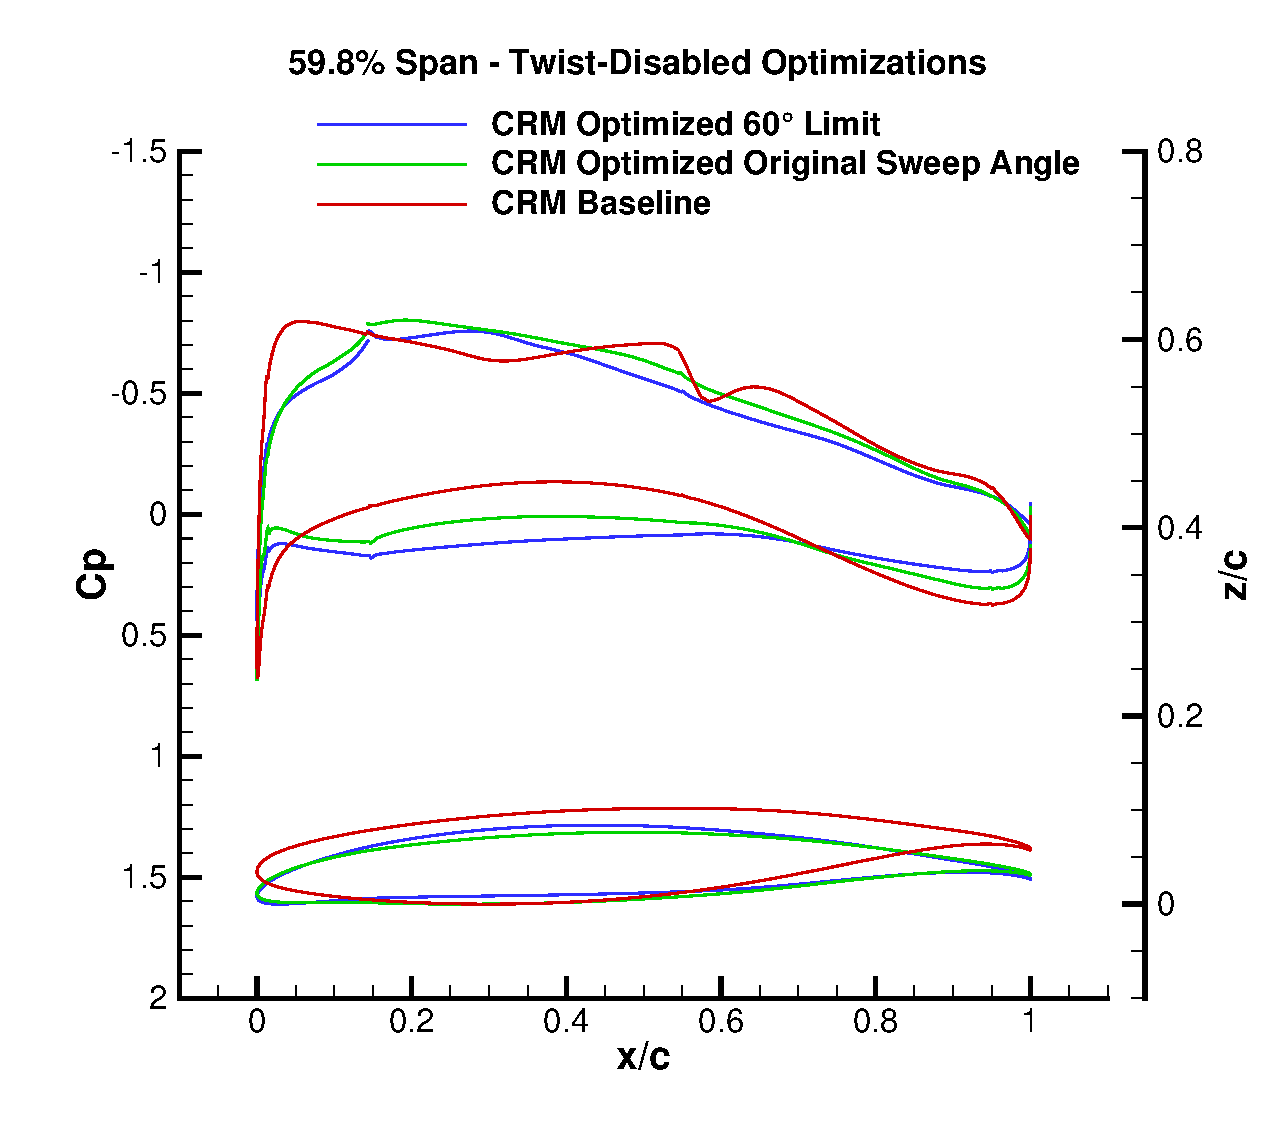
\includegraphics[trim={0.2cm 0.2cm 0.2cm 0.2cm},clip,width=3in]{Figures/No_Twist/NASA_CRM/NASA_CRM_Optimize_NoTwist-59.8percent_Span.eps}}\\
    \subfloat[\label{fig:crm_notwist_section_79.4_perc}]{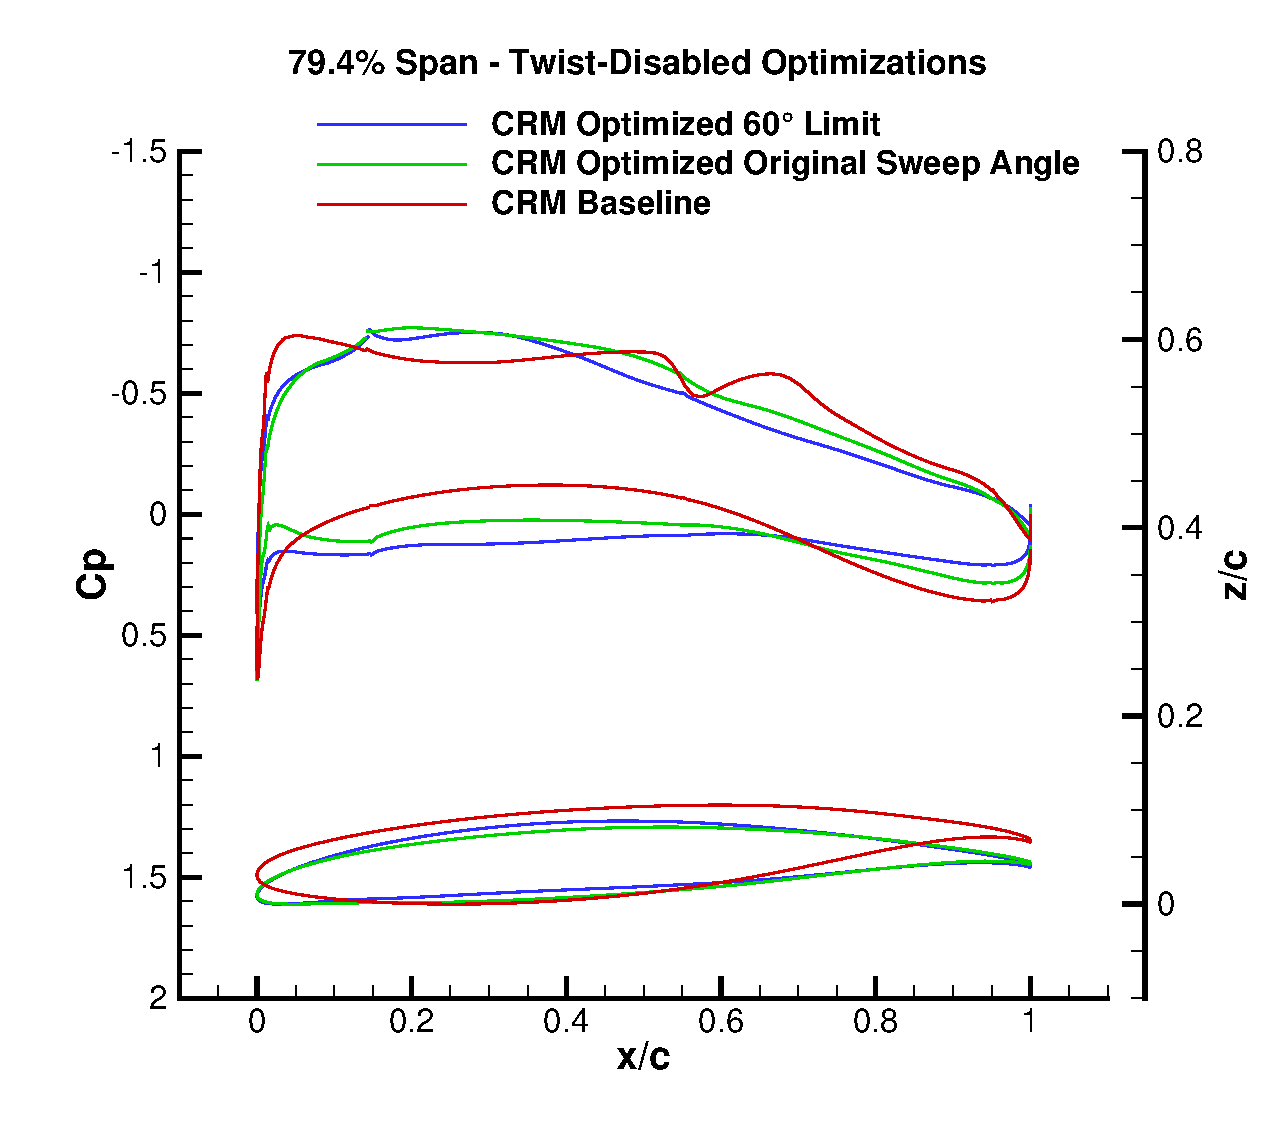
\includegraphics[trim={0.2cm 0.2cm 0.2cm 0.2cm},clip,width=3in]{Figures/No_Twist/NASA_CRM/NASA_CRM_Optimize_NoTwist-79.4percent_Span.eps}}
    \hspace{0.2cm}
    \subfloat[\label{fig:crm_notwist_section_99.0_perc}]{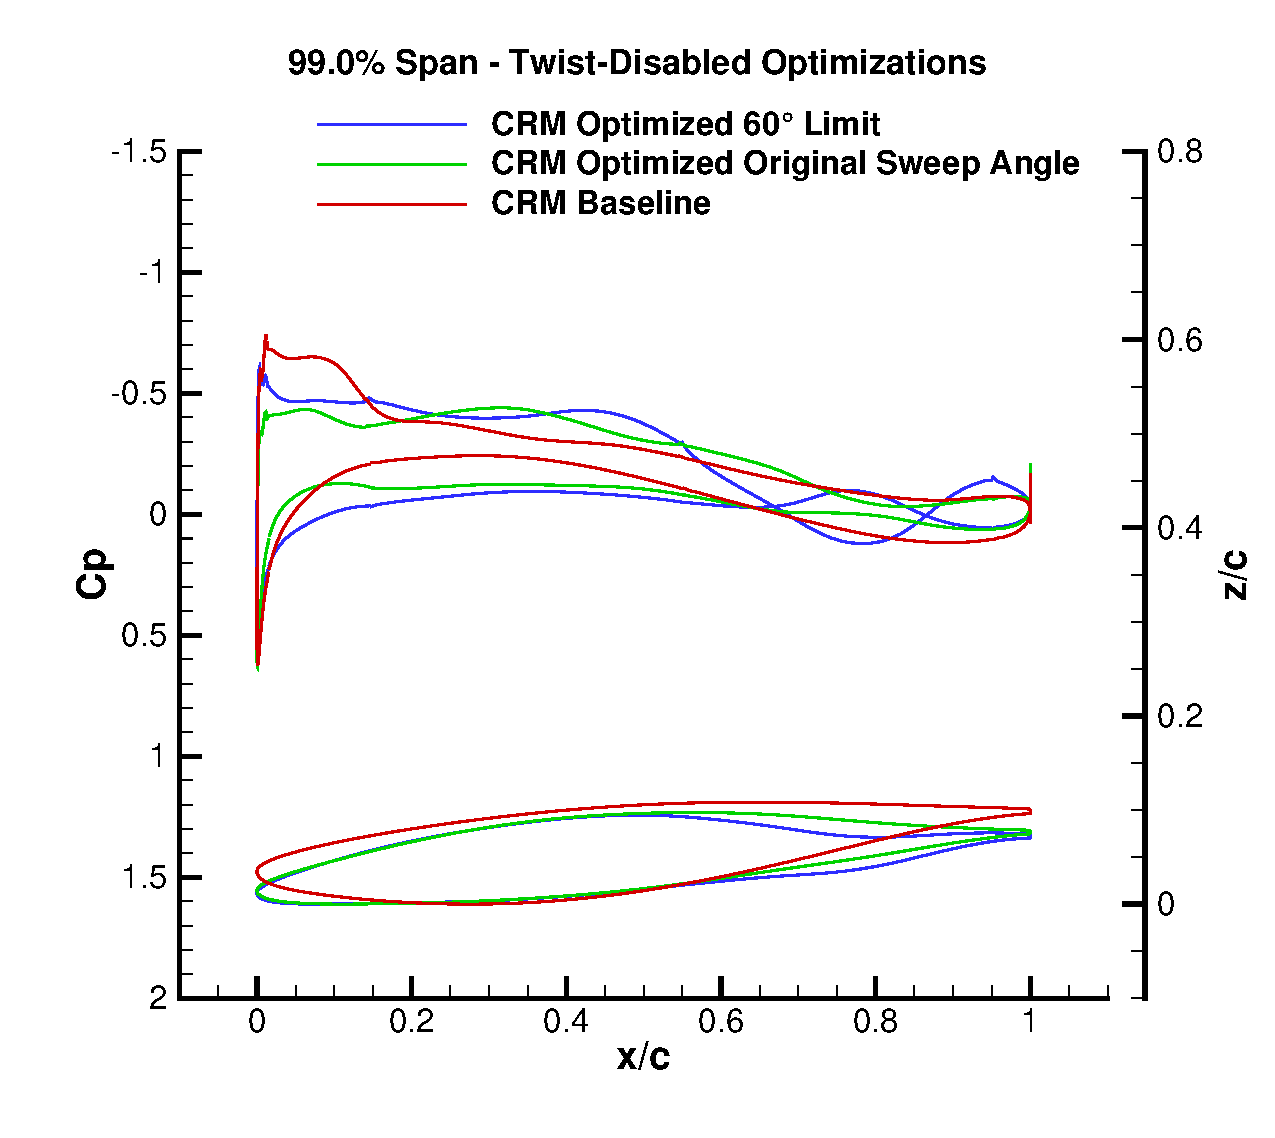
\includegraphics[trim={0.2cm 0.2cm 0.2cm 0.2cm},clip,width=3in]{Figures/No_Twist/NASA_CRM/NASA_CRM_Optimize_NoTwist-99.0percent_Span.eps}}
    \caption{Section geometry and pressure distribution plots of the trimmed angle of attack NASA CRM baseline planform, original sweep angle limit optimized planform, and 60.0\degree\ sweep angle limit optimized planform wihout wing twist in optimization at 1.00\% (\ref{fig:crm_notwist_section_1_perc}), 20.6\% (\ref{fig:crm_notwist_section_20.6_perc}), 40.2\% (\ref{fig:crm_notwist_section_40.2_perc}), 59.8\% (\ref{fig:crm_notwist_section_59.8_perc}), 79.4\%(\ref{fig:crm_notwist_section_79.4_perc}), and 99.0\% (\ref{fig:crm_notwist_section_99.0_perc}) span.}
\label{fig:crm_notwist_section_plots}
\end{figure}
\FloatBarrier

Compared to the trimmed baseline in Figure~\ref{fig:crm_baseline_planform}, the shock that occurs 60-80\% of the local chord on the upper surface of the wing in Figure~\ref{fig:crm_notwist_section_plots} is eliminated on both optimized planforms.
% Remove unnecessary detail
% As stated previously, the original geometry exhibits close clustering of pressure contour lines towards the trailing edge and a sharp drop in pressure that occurs between 60-80\% of the local chord on the upper surface of the wing in Figure~\ref{fig:crm_section_plots}, which is indicative of a shock along the entire span of the wing. Meanwhile, the absence of such characteristics on both optimized planforms indicates that both geometries are able to eliminate the shock wave, implying that wave drag is also substantially reduced or completely eliminated. Indeed, inspection of the section shape plots in Figure~\ref{fig:crm_notwist_section_plots} shows that the 60.0\degree\ sweep angle limit case is able to completely eliminate shocks over its entire span, as the pressure recovery is very smooth on the inboard sections of the wing. Strange behaviour is observed near the root for the 60.0\degree\ sweep angle limit case, where a cusp occurs on both the upper and lower surfaces. The source of this behaviour was unclear.
Notably, the optimization at the fixed sweep angle of 37.5\degree\ exemplifies a substantial improvement in shock characteristics over the trimmed baseline geometry without any changes to the wing sweep angle. One observes that that with the exception of the outboard sections of the wing, the pressure recovery is almost as smooth as that obtained in the 60.0\degree\ sweep angle limit case.
% In fact, it appears that this case is able to remove the shock waves as well.
% Minor perturbations exist during the pressure recovery at 79.4\% span as seen in Figure~\ref{fig:crm_notwist_section_79.4_perc}, but it is unclear why this has occurred. 

The section shapes for both the 37.5\degree\ fixed sweep angle and 60.0\degree\ sweep angle limit optimizations appear quite similar, with the 60.0\degree\ sweep angle limit simply appearing as a more exaggerated version of the former. 
% The negative camber towards the root is reduced in magnitude, which is similar to the 60.0\degree\ sweep angle limit case with wing twist. The camber is similarly reduced at 20.6\% span as well. Some differences to the twist-inclusive results appear in both the 37.5\degree\ fixed sweep angle and 60.0\degree\ sweep angle limit cases at 40.2\% span, where both cases have made the airfoil substantially thinner, as seen in Figure~\ref{fig:crm_notwist_section_40.2_perc}.
Changes to the airfoil's camber are complex—the airfoil reflex has been eliminated and the lower section flattened out. Meanwhile, the leading edge of the airfoil has lowered substantially, which maintains positive camber in the section shape despite the flattened lower section. Similar behaviour appears at 59.8\% and 79.4\% span in both twist-deactivated cases, as seen in Figures~\ref{fig:crm_notwist_section_59.8_perc} and~\ref{fig:crm_notwist_section_79.4_perc}. This lowering of the leading edge while flattening the lower section appears to be an attempt to modify the local twist on the wing without violating the the twist equality constraint of 0\degree. Indeed, converting the reflexed camber line to a positive camber line with a lowered leading edge visually appears to have this effect, showing that the optimizer is more than capable of exploiting the freedom given to it. 

The pressure coefficient behaviour and section shape results at the wingtip remain complex. Just as in the 60.0\degree\ sweep case with twist, odd changes to the airfoil have occurred along its entire length, seen in Figure~\ref{fig:crm_notwist_section_99.0_perc}.
% A reflexed camber line has been generated in the 60.0\degree\ sweep angle limit case without wing twist, with positive camber at the leading edge and negative camber towards the trailing edge, seen in Figure~\ref{fig:crm_notwist_section_99.0_perc}. It appears that the fixed-sweep optimization at 37.5\degree\ exhibits this behaviour as well, although less severely. 
It remains unclear why this behaviour has occurred, although as before, it does not appear in other studies on the CRM wing~\cite{martins_aerodynamic_2022, koo_investigation_2018, shi-dong_adjoint-based_2017, lyu_aerodynamic_2015, kenway_multipoint_2015} and may be attributed to the difference in locations along the wingspan used for plotting the section shape and $C_p$ in this study.

Alignment with the results of other studies is not possible for the optimization cases without wing twist. A search of relevant literature containing studies of the NASA CRM on a similar basis to this study make use of wing twist, including those conducted by by Koo and Zingg, Lyu et al., and Kenway et al.~\cite{koo_investigation_2018, lyu_aerodynamic_2015, kenway_multipoint_2015}, such that the results presented here are novel at the time of writing.

\section{A320neo Optimization}
\subsection{A320neo Optimization with Wing Twist}
\label{ssec:a320neo-opt-twist}
The initial optimization of the A320neo geometry was carried out using the procedure outlined in section~\ref{ssec-prob-formulate}. Similar to the CRM optimizations, the initial choices in the upper wing sweep angle limit proved to be too low. The 45.5\degree sweep limit was expanded to 50.0\degree, and then expanded again to 60.0\degree to ensure a sufficient margin between the resultant wing sweep angle and the upper limit. The convergence history and and results for all three sweep angle limits are provided for completeness, and are presented in Figures~\ref{fig:a320neo_converge_45.5_Deg},~\ref{fig:a320neo_converge_50.0_Deg},~\ref{fig:a320neo_converge_60.0_Deg}, and Table~\ref{tab:a320neo_results}.

% Observation of the design variable history during optimization iterations illustrated that the wing sweep rose to its upper limit of 37.7\degree\ within 60 iterations and remained there. The optimization was manually stopped after 88 design iterations. Analysis of the merit function, optimality, and feasibility of this study illustrated that this case was not converged, as seen in Figure~\ref{fig:a320neo_converge_45.5_Deg}.

\begin{figure}[!tp]
    \centering
    \subfloat[\label{fig:a320neo_converge_45.5_Deg}]{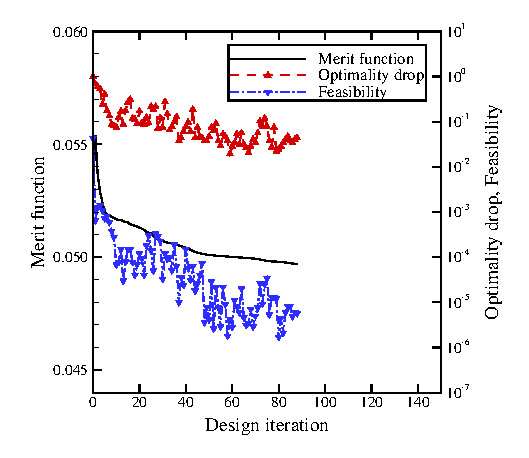
\includegraphics[trim={0.15cm 0cm 0.15cm 0cm},clip,width=3.175in]{Figures/With_Twist/A320neo/optimize_A320neo.eps}}
    \hspace{0.25cm}
    \subfloat[\label{fig:a320neo_converge_50.0_Deg}]{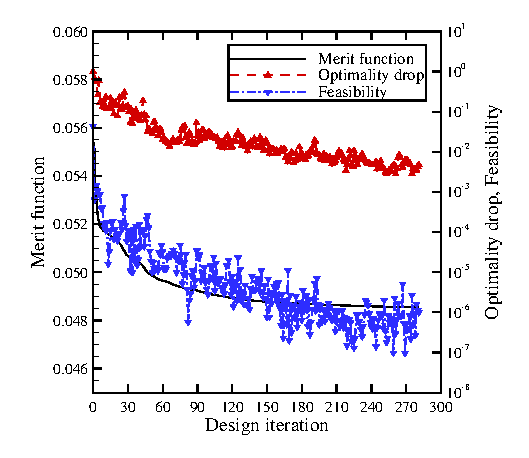
\includegraphics[trim={0.15cm 0cm 0.15cm 0cm},clip,width=3.175in]{Figures/With_Twist/A320neo/Optimize_A320_50deg.eps}}
    \caption{Convergence history for A320neo optimization with an upper sweep angle limit of 45.5\degree (\ref{fig:a320neo_converge_45.5_Deg}) and 50.2\degree (\ref{fig:a320neo_converge_50.0_Deg}).}
\label{fig:a320neo_planform_plots}
\end{figure}

% Similar to the NASA CRM's initial sweep optimization case, it was clear that this geometry has a very strong tendency to increase the wing sweep even further, as evidenced by the active wing sweep constraint very early on in the optimization. Performance also greatly increased when compared to a baseline trimmed flow solution for the same geometry, which was trimmed to an angle of attack that would satisfy the lift lift constraint of $C_L S=1.6686$, as seen in Table~\ref{tab:a320neo_results}. The drag coefficient $C_D S$ decreased by 101.1 drag counts with a small decrease in angle of attack. The $L/D$ also increased by over 5, from 27.89 to 33.58. This substantial improvement in efficiency motivated the decision to halt the optimization and start a new case with an increased sweep angle limit, as better performing optimum may be located at higher sweep angles, which was seen in the CRM optimization.

% As in the CRM optimization cases, the second A320neo case was run with a sweep angle limit expanded to 50.0\degree, which after converting to units of MAC and truncating, resulted in an upper sweep angle limit of 50.2\degree.
% This case was run for over 250 iterations. Continual decreases in the merit function, optimality, and feasibility were observed, as seen in Figure~\ref{fig:a320neo_converge_50.0_Deg}.

\begin{figure}[!tp]
\centering
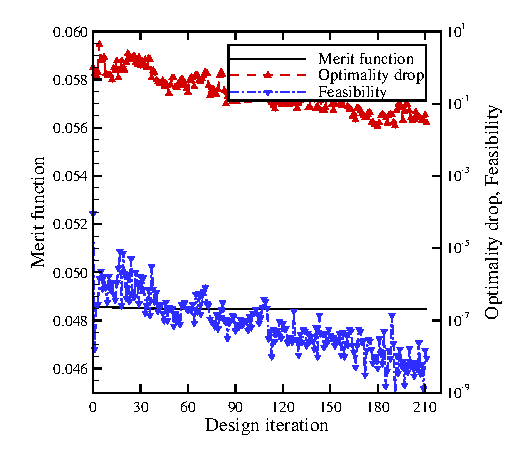
\includegraphics[width=4.5in]{Figures/With_Twist/A320neo/Optimize_A320_60deg.eps}
\caption{Convergence history for A320neo optimization with an upper sweep angle limit of 60.0\degree.}
\label{fig:a320neo_converge_60.0_Deg}
\end{figure}

% The merit function was seen to exhibit asymptotic behaviour after 150 design iterations, indicating that this case may have settled into a optimum. However, analysis of the optimization iteration history illustrated that just as in the CRM 50.0\degree\ case, the optimized geometry possesses a sweep angle close to the sweep angle limit of 50.2\degree, albeit not as close as the CRM 50.0\degree\ case. The sweep angle had increased to 46.90\degree, with corresponding improvements in $C_D S$ by 11.5 drag counts. The angle of attack increased by 0.056\degree, increasing from 2.103\degree\ to 2.159\degree—behaviour opposite to the CRM's trends. When converted to units of MAC, the margin between the optimized sweep angle and the upper sweep angle limit was 0.5385 reference units. This value is a much higher margin compared to the CRM 50.0\degree\ case, corresponding to approximately 20\% of the A320neo's 50.0\degree\ sweep limit of 2.750 reference units. The A320neo's sweep limit constraint was certainly inactive in this instance but it was decided that the sweep angle should be increased further to be thorough.

% The last A320neo case made use of the last optimized geometry from the 50.2\degree\ sweep limit case as its initial geometry. The upper sweep limit was expanded further to 60.0\degree, resulting in modifications to the upper sweep angle constraint as seen in Table~\ref{tab:a320neo-opt-60deg}.

\begin{table}[!tp]
\centering
\caption{Results summary for the optimization of the A320neo}
\label{tab:a320neo_results}
\begin{adjustbox}{center}
\begin{tabular}{lcccc}
\hline\hline
Design Variable & Trimmed Baseline & 37.7\degree\ Sweep Limit & 50.2\degree\ Sweep Limit & 60.0\degree\ Sweep Limit\\
\hline
$S$ (ref. units\textsuperscript{2}) & 3.340 & 3.339 & 3.339 & 3.338 \\
$C_L S$ & 1.669 & 1.669 & 1.669 & 1.669 \\
$C_M S$ & -0.736 & -1.399 & -2.280 & -2.254 \\
$C_D S$ (counts) & 598.2 & 497.0 & 485.5 & 484.7 \\
$L/D$ & 27.89 & 33.58 & 34.37 & 34.42 \\
Angle of Attack & 2.303\degree\ & 2.103\degree\ & 2.159\degree\ & 2.026\degree\ \\
\makecell[l]{Post-Optimization\\Leading Edge Sweep Angle} & 27.9\degree\ & 37.68\degree\ & 46.90\degree\ & 46.74\degree\ \\
\hline\hline
\end{tabular}
\end{adjustbox}
\end{table}

% This case was run for over 200 iterations, and observed no significant changes to the merit function. The optimality dropped one order of magnitude, whereas the feasibility decreased by three orders of magnitude to approximately $10^{-9}$, as seen in Figure~\ref{fig:crm_converge_60.0_Deg}. 

The result from the 60.0\degree\ sweep limit case indicates that it is simply a further convergence on the result from the 50.2\degree\ case. The geometry did not change significantly compared to the 50.2\degree\ sweep limit case. Just as in the CRM 60.0\degree\ case, the sweep limit decreased from the A320neo 50.2\degree\ case's most optimal point, dropping 0.16\degree\ from 46.90\degree\ to 46.64\degree, as seen in Table~\ref{tab:a320neo_results}. Performance compared to the trimmed baseline shows that the $C_D S$ decreased by 113.4 drag counts to 484.7, the $L/D$ increased by 6.52 to 34.42, and the angle of attack decreased by 0.277\degree\ to 2.026\degree. Plots of the upper surface pressure contours for the trimmed baseline flow solution and the 60.0\degree\ sweep limit optimized planform are shown in Figure~\ref{fig:a320neo_planform_plots}. Plots of the section geometry and pressure distribution at various spanwise sections for the trimmed baseline flow solution and the 60.0\degree\ sweep limit optimized planform are shown in Figure~\ref{fig:a320neo_section_plots}.

Just as in the CRM case, the A320neo's original geometry exhibits a shock along the entire span of the wing, as seen in Figures~\ref{fig:a320neo_baseline_planform} and~\ref{fig:a320neo_section_plots}. The optimized geometry resulting from the 60.0\degree\ sweep limit is able to completely remove this shock. Furthermore, with the exception of the root and wingtip, the optimizer is able to produce a smooth pressure recovery over the wing, as seen in Figures~\ref{fig:a320neo_section_20.6_perc}-\ref{fig:a320neo_section_79.4_perc}.

\begin{figure}[!tp]
    \centering
    \subfloat[\label{fig:a320neo_baseline_planform}]{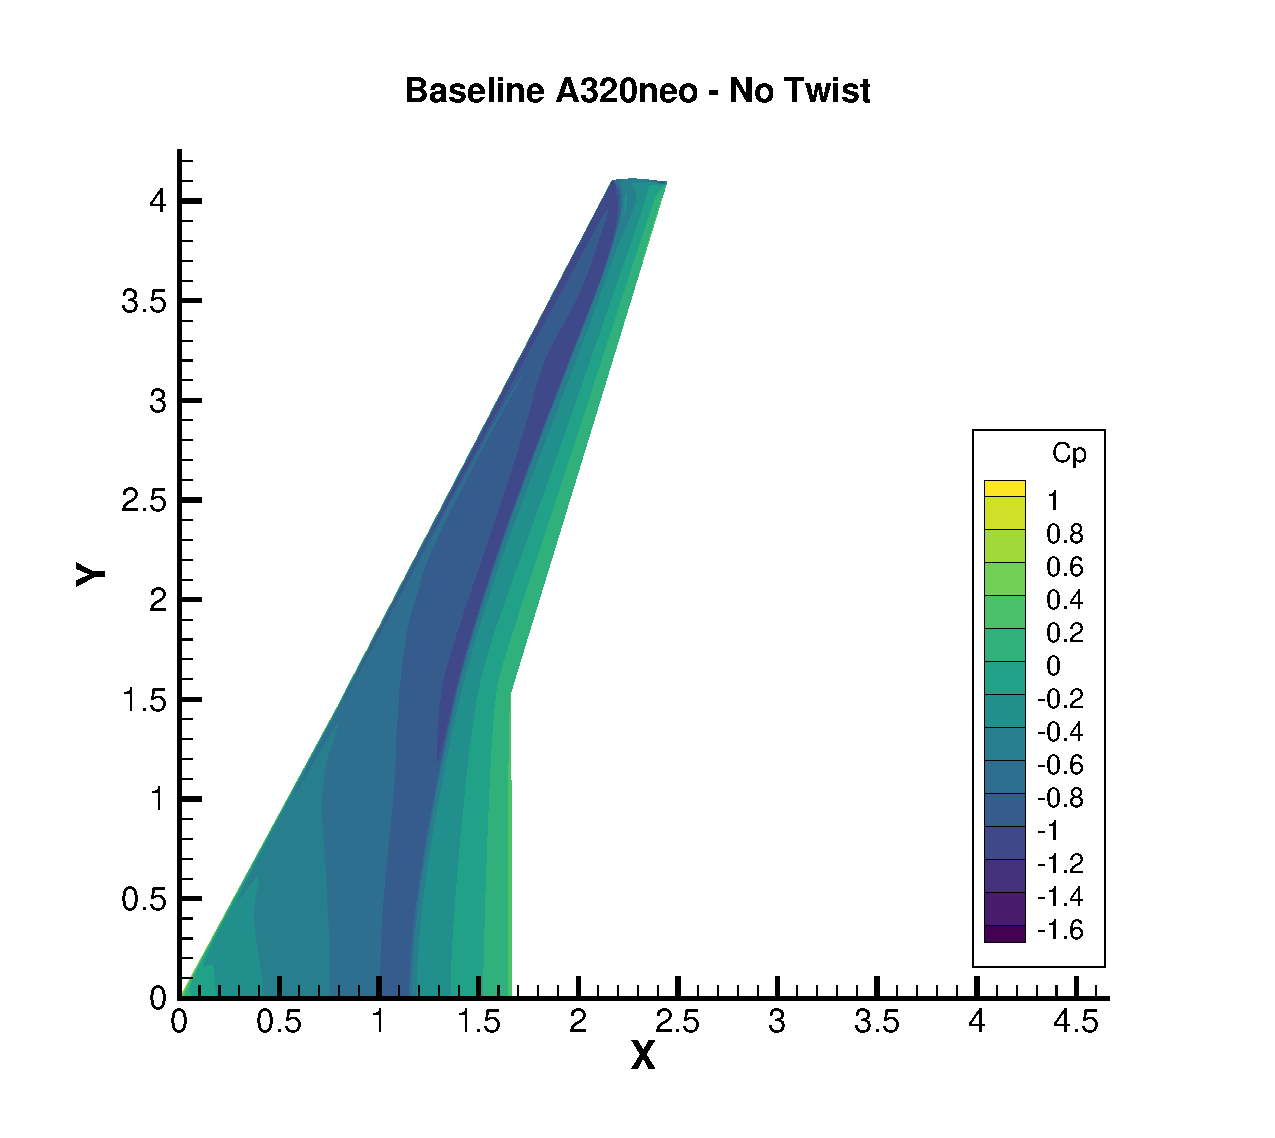
\includegraphics[trim={0.25cm 0.25cm 0.25cm 0.25cm},clip,width=3.175in]{Figures/With_Twist/A320neo/A320neo_Baseline-Contour-Upper.eps}}
    \hspace{0.25cm}
    \subfloat[\label{fig:a320neo_60_deg_planform}]{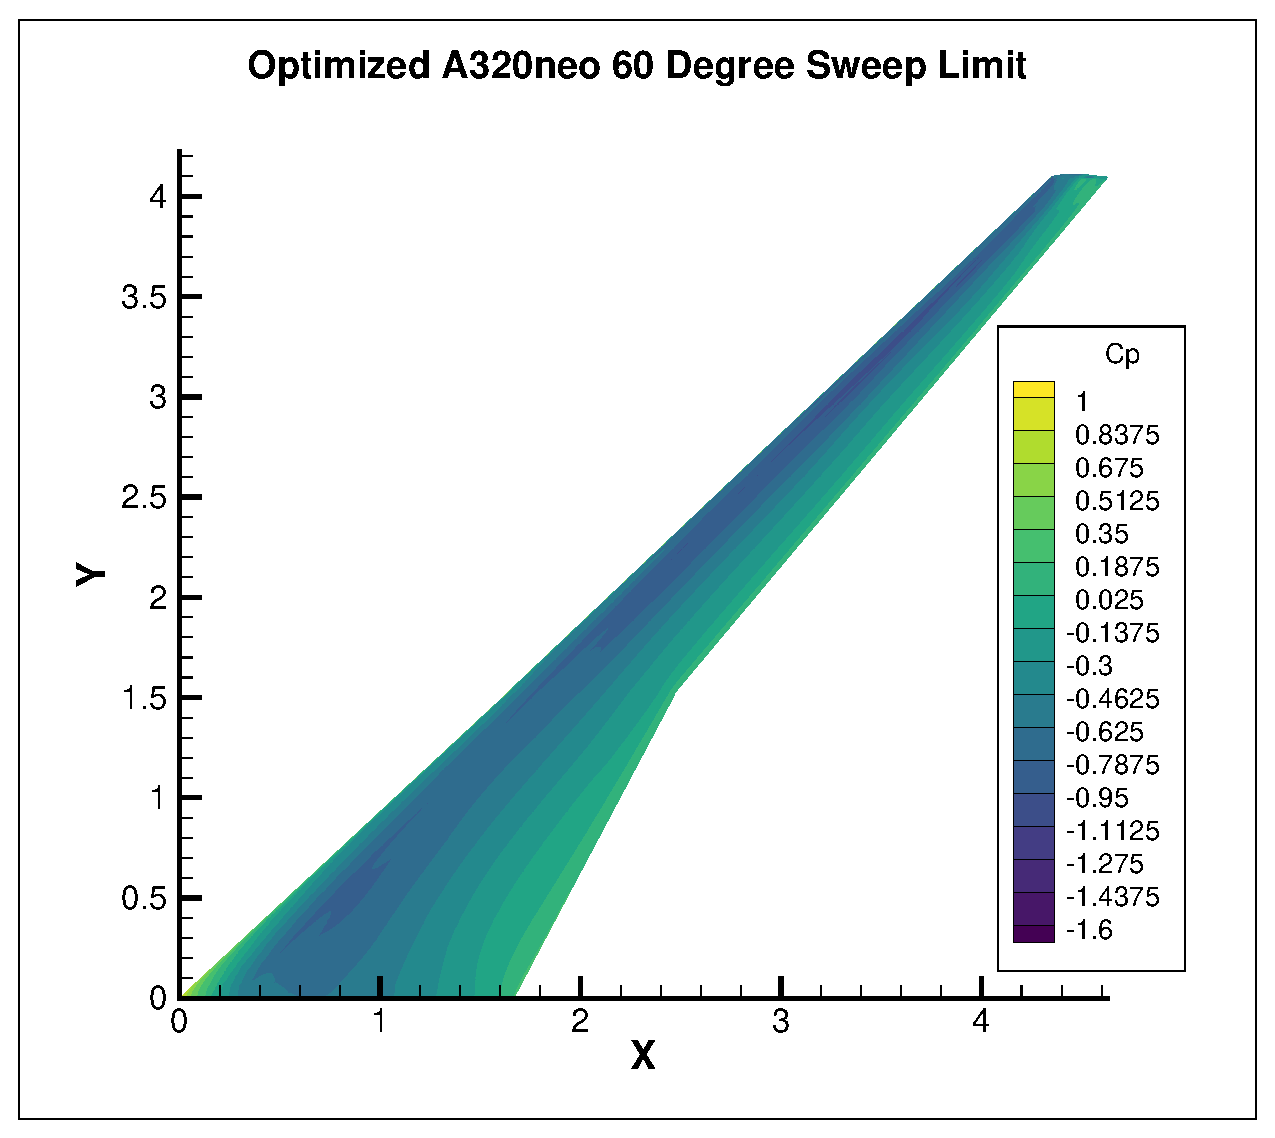
\includegraphics[trim={0.25cm 0.25cm 0.25cm 0.25cm},clip,width=3.175in]{Figures/With_Twist/A320neo/A320neo_varsweep_60deg-Contour-Upper.eps}}
    \caption{A320neo upper surface pressure contours for the trimmed angle of attack baseline planform (\ref{fig:a320neo_baseline_planform}) and 60.0\degree\ sweep angle limit optimized planform (\ref{fig:a320neo_60_deg_planform}).}
\label{fig:a320neo_planform_plots}
\end{figure}

\begin{figure}[!tp]
    \centering
    \subfloat[\label{fig:a320neo_section_1_perc}]{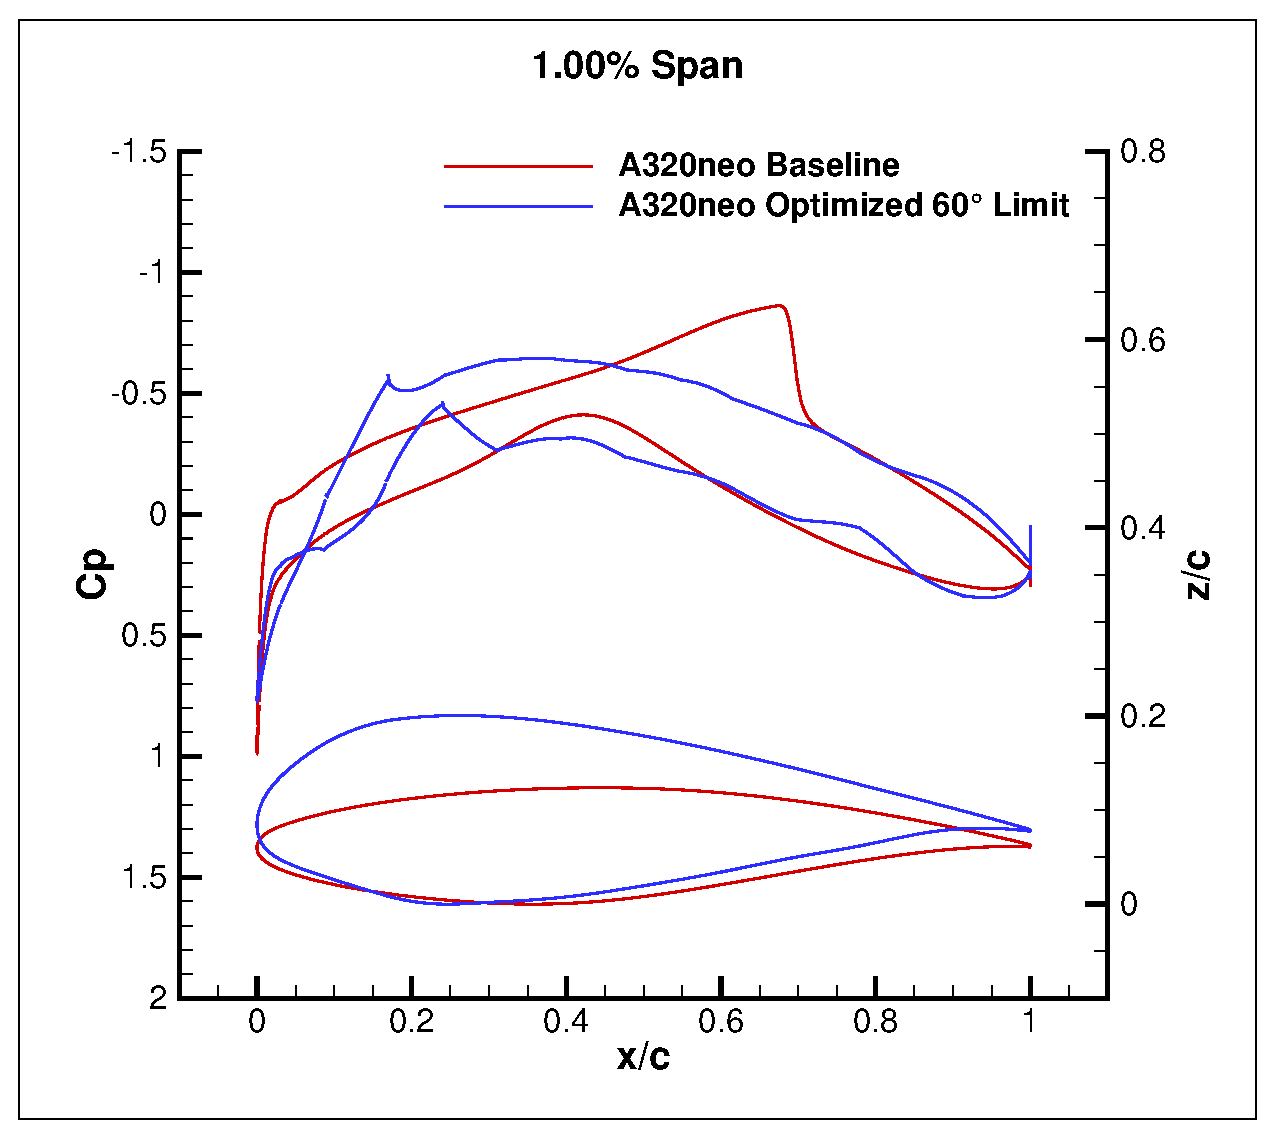
\includegraphics[trim={0.25cm 0.25cm 0.25cm 0.25cm},clip,width=3in]{Figures/With_Twist/A320neo/A320neo_1.00percent_Span.eps}}
    \hspace{0.25cm}
    \subfloat[\label{fig:a320neo_section_20.6_perc}]{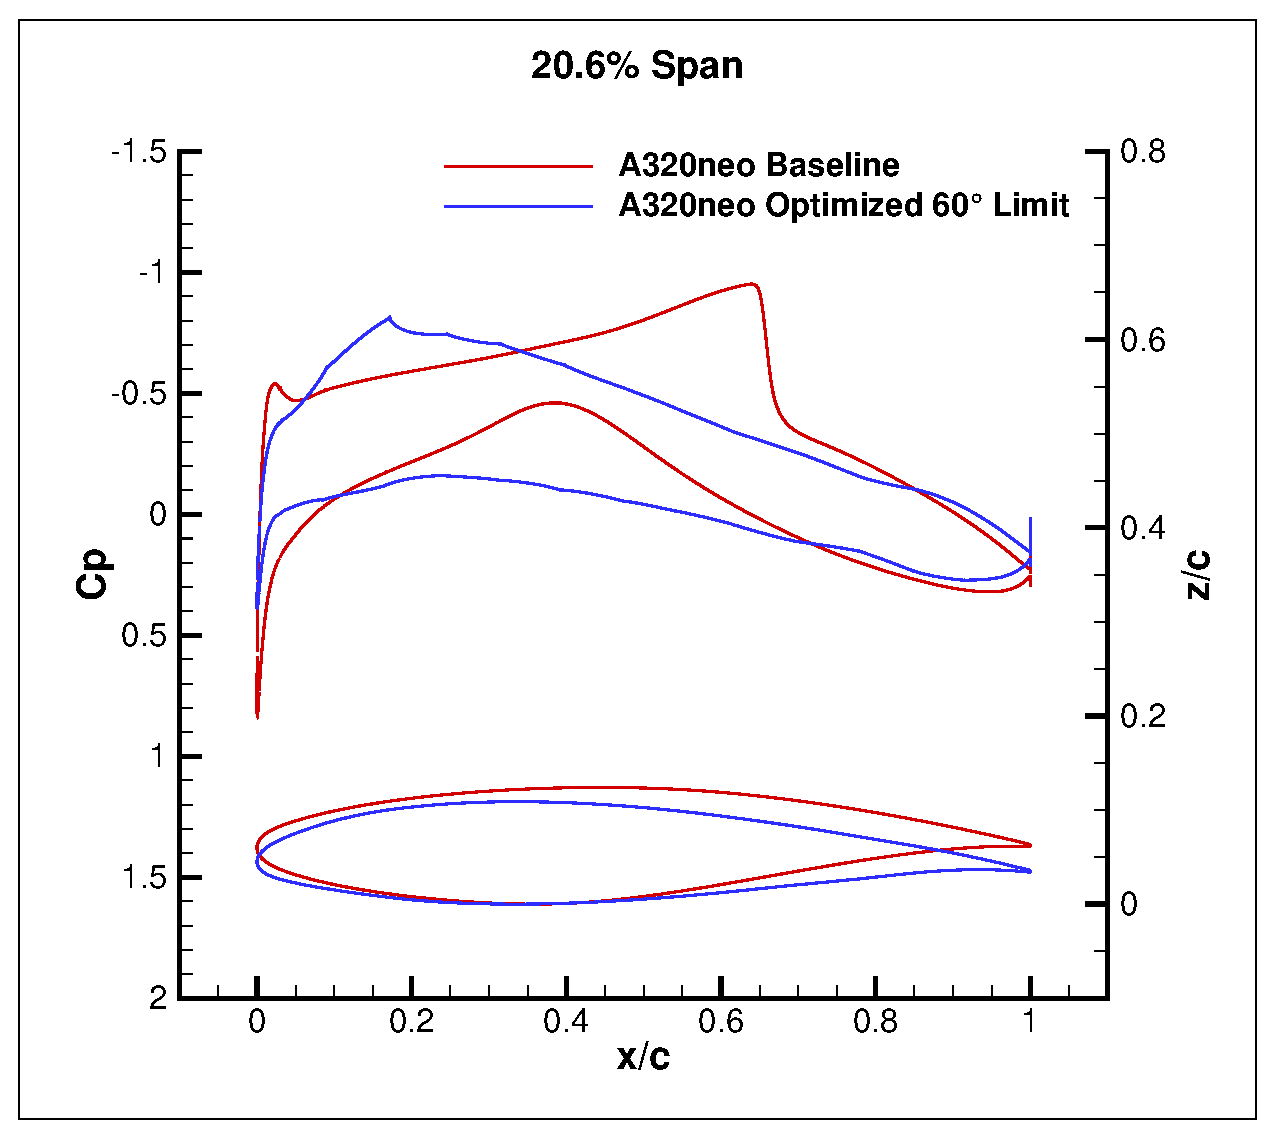
\includegraphics[trim={0.25cm 0.25cm 0.25cm 0.25cm},clip,width=3in]{Figures/With_Twist/A320neo/A320neo_20.6percent_Span.eps}}\\
    \subfloat[\label{fig:a320neo_section_40.2_perc}]{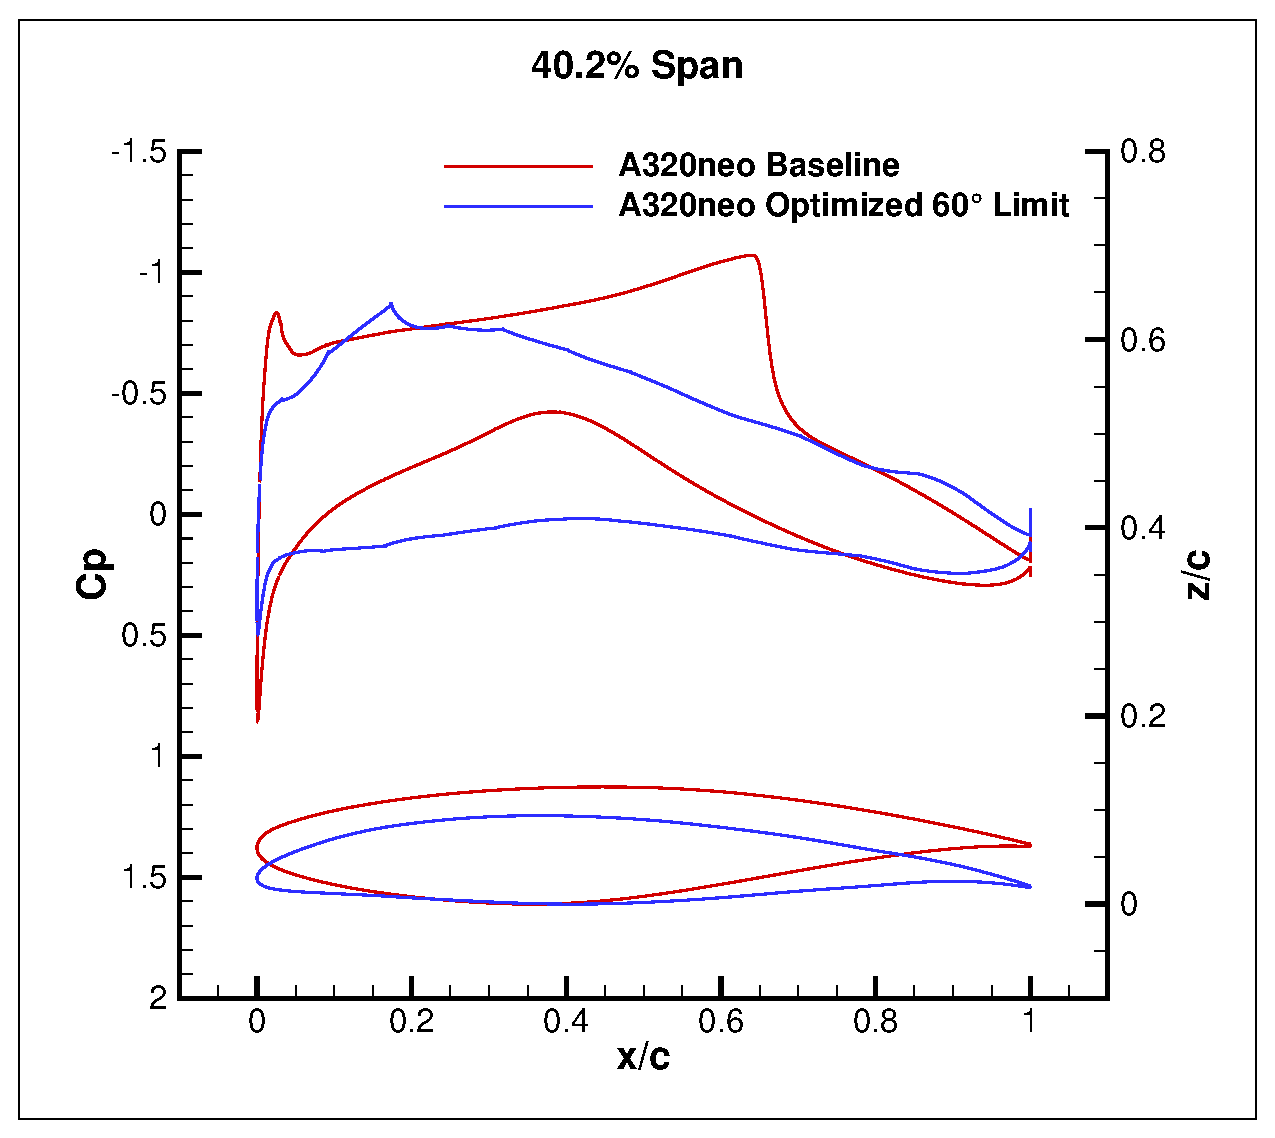
\includegraphics[trim={0.25cm 0.25cm 0.25cm 0.25cm},clip,width=3in]{Figures/With_Twist/A320neo/A320neo_40.2percent_Span.eps}}
    \hspace{0.25cm}
    \subfloat[\label{fig:a320neo_section_59.8_perc}]{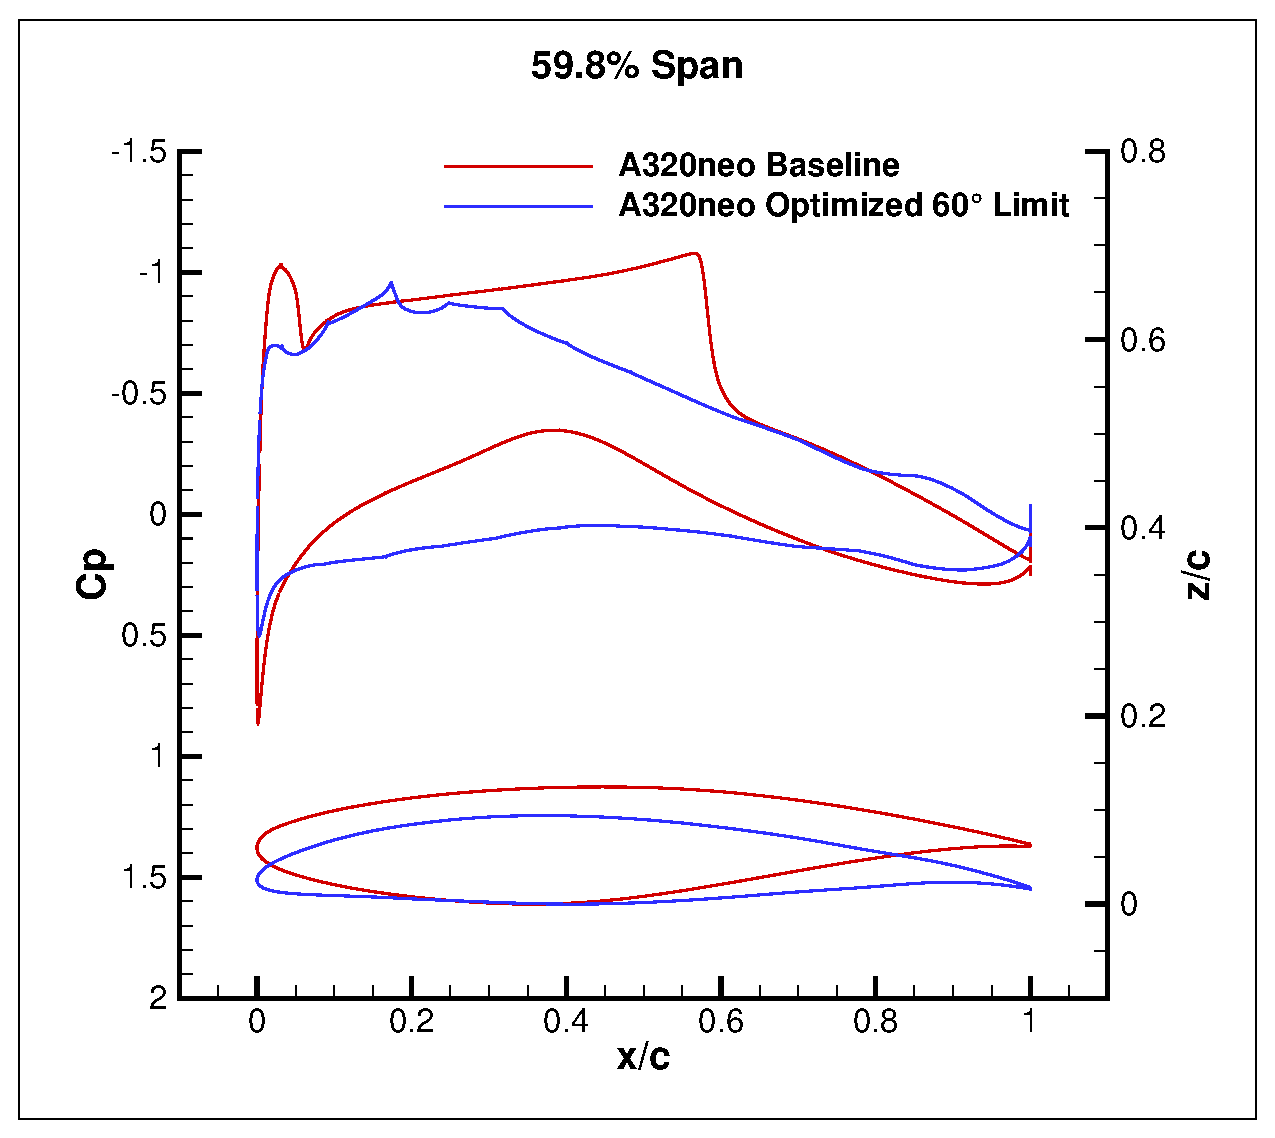
\includegraphics[trim={0.25cm 0.25cm 0.25cm 0.25cm},clip,width=3in]{Figures/With_Twist/A320neo/A320neo_59.8percent_Span.eps}}\\
    \subfloat[\label{fig:a320neo_section_79.4_perc}]{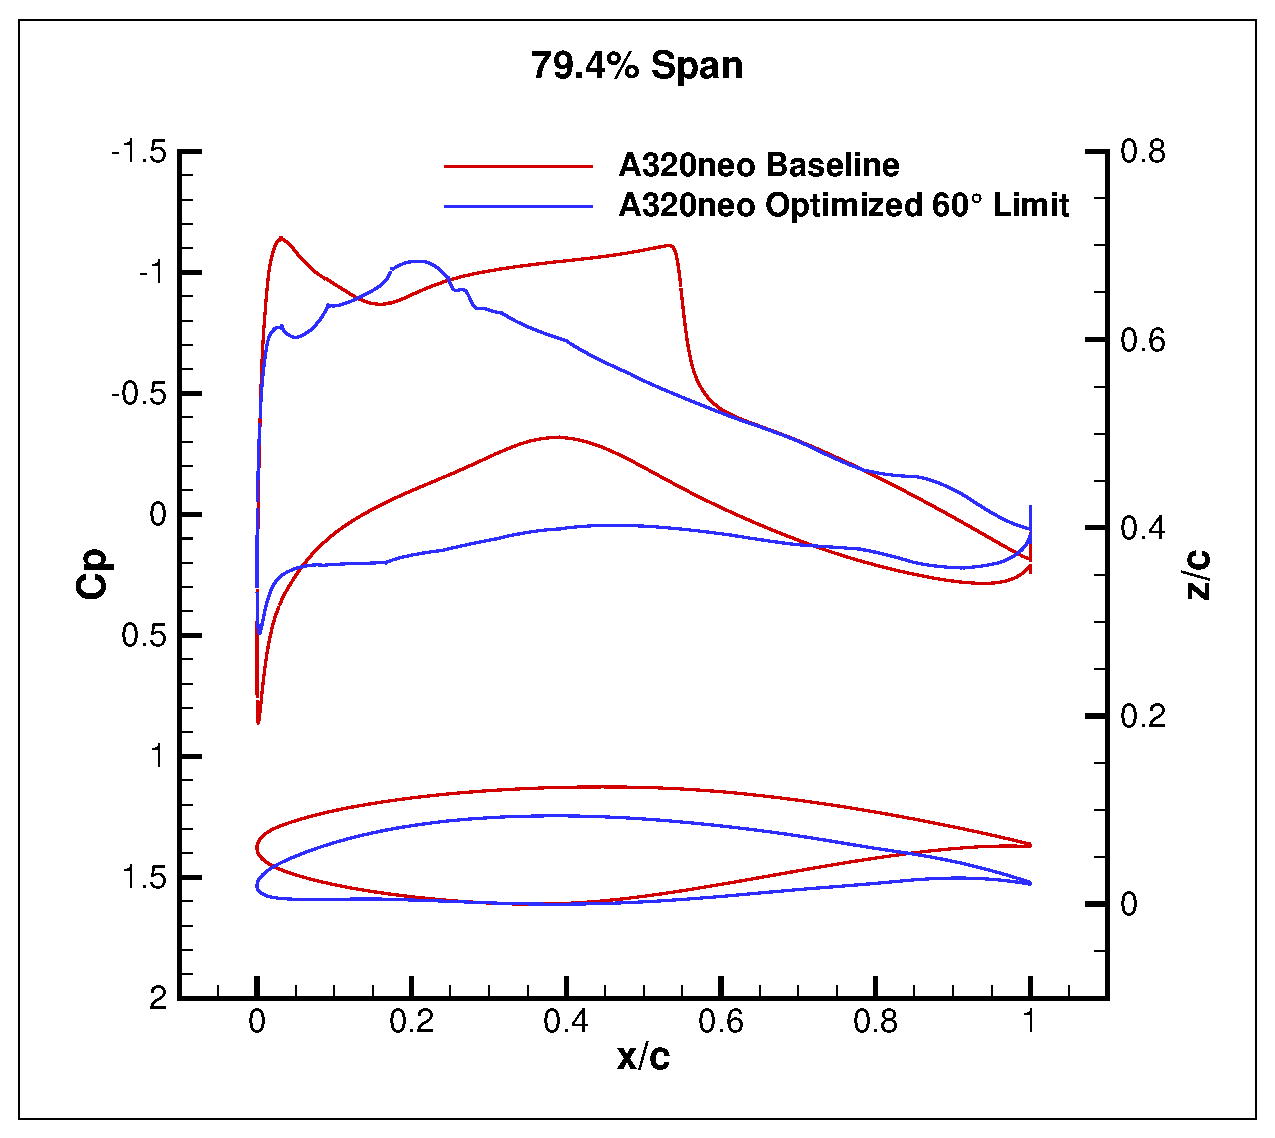
\includegraphics[trim={0.25cm 0.25cm 0.25cm 0.25cm},clip,width=3in]{Figures/With_Twist/A320neo/A320neo_79.4percent_Span.eps}}
    \hspace{0.25cm}
    \subfloat[\label{fig:a320neo_section_99.0_perc}]{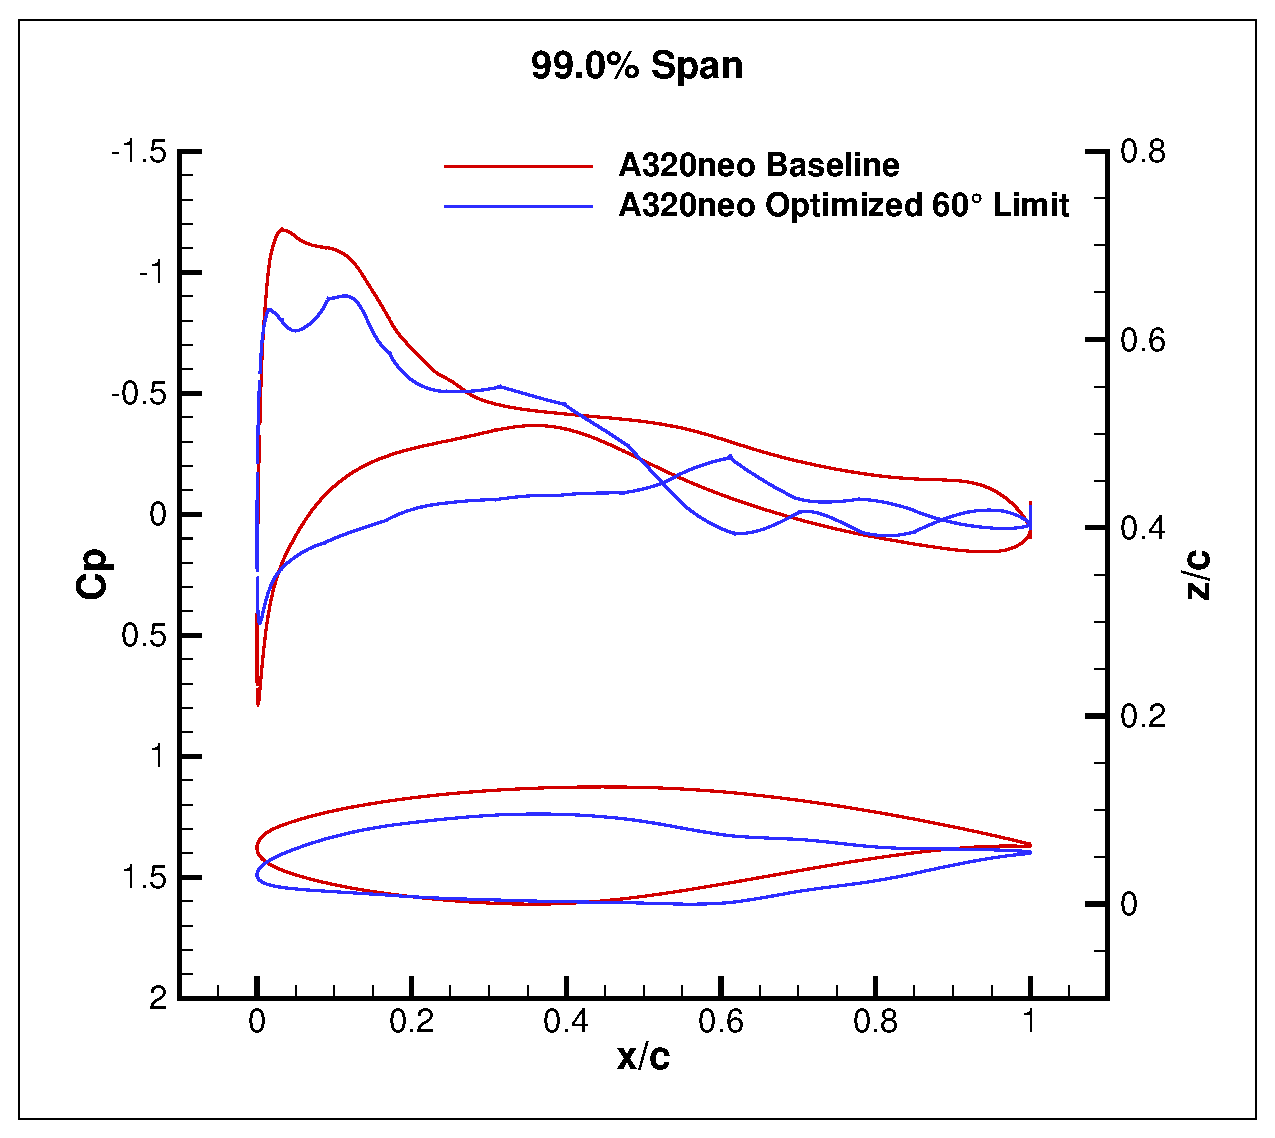
\includegraphics[trim={0.25cm 0.25cm 0.25cm 0.25cm},clip,width=3in]{Figures/With_Twist/A320neo/A320neo_99.0percent_Span.eps}}
    \caption{Section geometry and pressure distribution plots of the trimmed angle of attack A320neo baseline planform and 60.0\degree\ sweep angle limit optimized planform at 1.00\% (\ref{fig:a320neo_section_1_perc}), 20.6\% (\ref{fig:a320neo_section_20.6_perc}), 40.2\% (\ref{fig:a320neo_section_40.2_perc}), 59.8\% (\ref{fig:a320neo_section_59.8_perc}), 79.4\%(\ref{fig:a320neo_section_79.4_perc}), and 99.0\% (\ref{fig:a320neo_section_99.0_perc}) span.}
\label{fig:a320neo_section_plots}
\end{figure}
\FloatBarrier

The section shape of the optimized wing differs greatly from the baseline geometry, although in slightly different ways compared to the CRM optimized wing. The thickness is greatly increased at the root and is continuously reduced along the remainder of the wingspan compared to the initial geometry. Since this case included a minimum volume constraint, this behaviour is expected and aligns with the results of other studies~\cite{ledoux_study_2015, kenway_multipoint_2015, telidetzki_application_2014, lyu_rans-based_2014, lyu_aerodynamic_2015, osusky_drag_2015, shi-dong_approximate_2018, yu_influence_2018, koo_investigation_2018}. The camber is reduced at almost all spanwise points with the exception of the wingtip, where strange behaviour occurs. As seen in Figure~\ref{fig:a320neo_section_99.0_perc}, a complex section shape is produced. This feature is similar to the wingtip section shape produced in the CRM 60.0\degree\ twist-inclusive optimization case, and it is unclear why it occurred in this case as well.
% However, the trailing half of the wing appears to be at a greater twist relative to the CRM section at 79.4\% span in Figure~\ref{fig:crm_section_79.4_perc}, which differs compared to the CRM case. The overall twist at 99.0\% span appears to be a marginal increase compared to the original geometry, but it is unclear why this result has occurred. 
Just as in the CRM case, the spanwise sections used for measurement in this study differ from those specified in ADODG Case 4 and reported in other studies~\cite{martins_aerodynamic_2022, koo_investigation_2018, shi-dong_adjoint-based_2017, lyu_aerodynamic_2015, kenway_multipoint_2015}, such that the root and wingtip sections measured in this study are not the same as those used in ADODG Case 4. Again, it is possible that analysis of the sections using the spanwise points dictated by ADODG Case 4 may show that such artifacts do not occur when measuring at 94.4\% span as specified by ADODG Case 4, compared to measurements at 99.0\% span as used in this study.

%%%%%%%%%%%%%%%%%% TALK ABOUT WEIRD TWIST BEHAVIOUR HERE %%%%%%%%%%%%%%%%%%
The wing artifact occurring at 99.0\% span seen in the NASA CRM geometry also occurs on the A320neo, as seen in Figure~\ref{fig:a320neo_section_99.0_perc}. Oscillations in wing twist occurred as well, as seen in Figure~\ref{fig:a320neo_artifact}. These oscillations are lower in amplitude compared to those seen on the NASA CRM 60.0\degree\ case with wing twist. Just as in the NASA CRM study, a secondary optimization was conducted on the A320neo with an otherwise identical methodology to that in section~\ref{ssec-prob-formulate}, with the exception of wing twist as a design variable and the selection of sweep limits, which are described in the following section.

\begin{figure}[!tp]
    \centering
    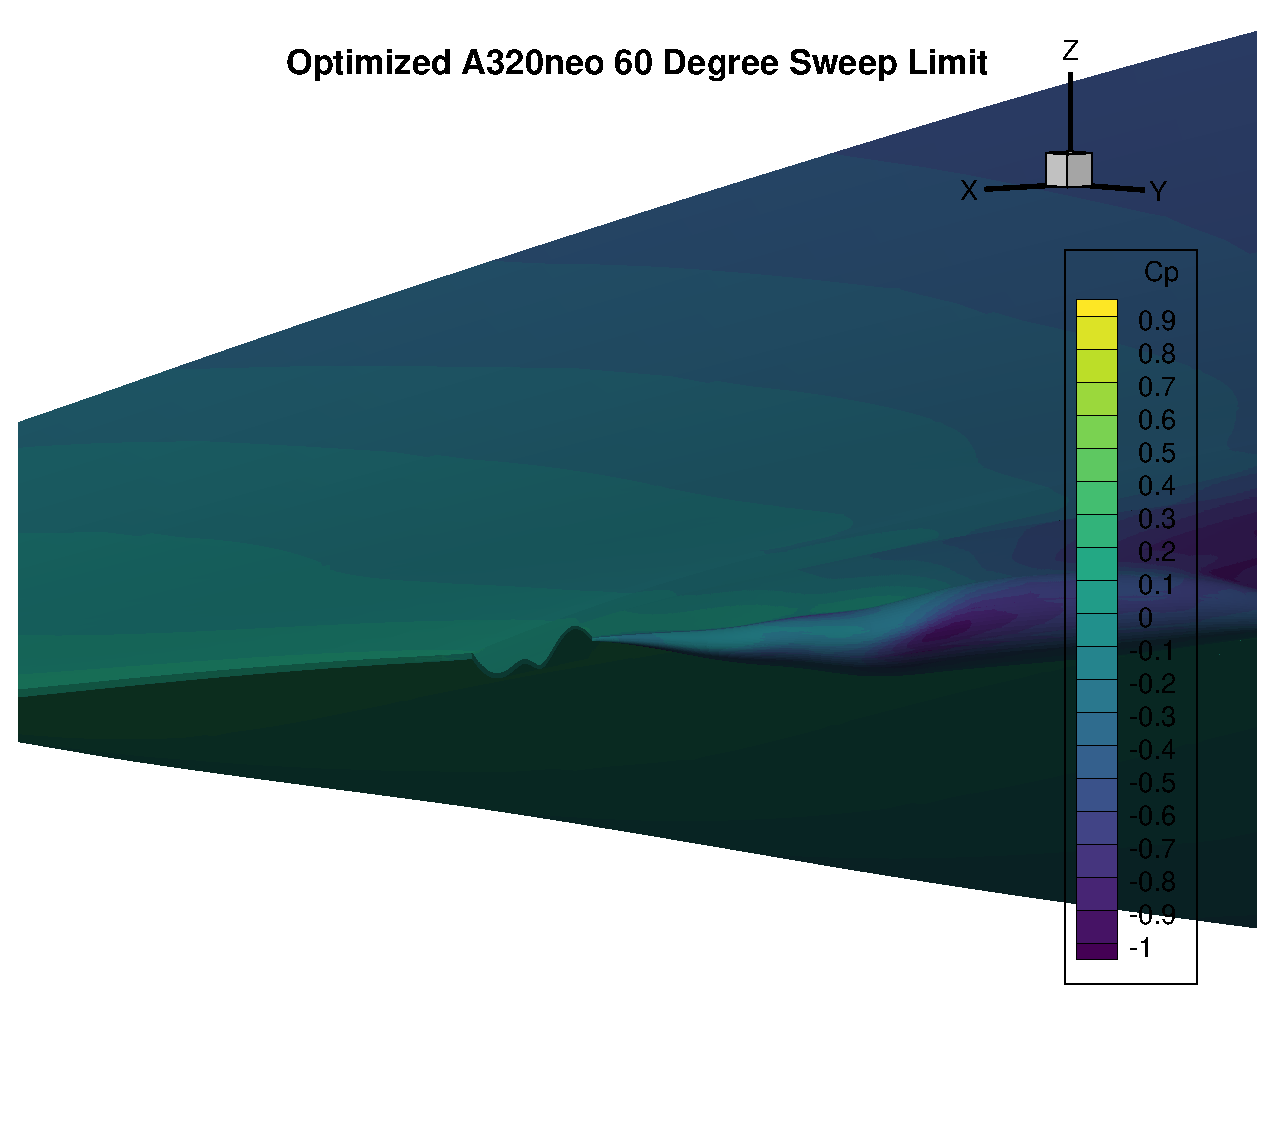
\includegraphics[width=4.5in]{Figures/With_Twist/A320neo/Optimize_A320_60deg_Twist_Artifact_01.eps}
    \caption{Trailing edge geometry artifacts observed in the A320neo 60.0\degree\ sweep angle limit optimized planform.}
\label{fig:a320neo_artifact}
\end{figure}
\FloatBarrier

%%%%%%%%%%%%%%%%%% INTRODUCE NEW CASE WITHOUT TWIST %%%%%%%%%%%%%%%%%%

\subsection{A320neo Optimization without Wing Twist}
\label{ssec:a320neo-opt-notwist}
Similar to the twist-deactivated study performed on the CRM wing, a second study was performed on the A320neo without wing twist as a design variable. In these cases, the local wing twist was required to be equal to 0\degree\ every where on the wing. Based on the results obtained in the initial A320neo ASO cases, the sweep angle limit was expanded to 60.0\degree.

An additional study was conducted on the A320neo without wing twist at its original sweep angle of 27.9\degree\ as well. Just as in the CRM twist-deactivated cases, this optimization result served to provide context for the 60.0\degree\ sweep limit result without wing twist, as ASO on section shape and angle of attack at an aircraft's original sweep angle is the most accessible way to performance on a conventional aircraft, and is also the approach that is conducted most often~\cite{lyu_rans-based_2014, lyu_aerodynamic_2015, osusky_drag_2015, streuber_investigation_2017, koo_investigation_2018}. Wing twist is typically included as well, but the geometry artifacts obtained when twist was included as a design variable motivated its exclusion from a fixed sweep angle ASO at the A320neo's original sweep angle.

The fixed sweep angle A320neo ASO at the original sweep angle of 27.9\degree\ exhibited smooth optimization progress, with qualitative analysis of the merit function, optimality, and feasibility demonstrating that convergence was obtained after 326 design iterations, as seen in Figure~\ref{fig:a320neo_notwist_converge_baseline}. The drag coefficient $C_D S$ decreased by 98.5 drag counts relative to the trimmed baseline wing, the $L/D$ increased by 5.5, and the angle of attack decrease by over 0.5\degree, as seen in Table~\ref{tab:a320neo_notwist_results}.

The A320neo ASO without twist at a sweep angle limit of 60.0\degree\ demonstrated similarly smooth optimization progress compared to the previous twist-deactivated case. Analysis of the merit function, optimality, and feasibility illustrated that convergence was achieved after 388 design iterations, as seen in Figure~\ref{fig:a320neo_notwist_converge_60.0_Deg}. The drag coefficient decreased by 112.6 drag counts relative to the trimmed baseline wing, with a less than 0.1\degree\ decrease in the angle of attack. The moment coefficient decreased considerably by over 1.5, lowering from -0.736 to -2.268. The $L/D$ increased by almost 6.5 counts, rising from 27.89 to 34.37. While this is a substantial improvement over the trimmed baseline wing, it is only a 2.83\% improvement over the A320neo optimized at the original sweep angle of 27.9\degree, despite an increase in the wing sweep of almost 19\degree.

%%%%%% A320neo NO TWIST CONVERGENCE PLOTS %%%%%%
\begin{figure}[!tp]
\centering
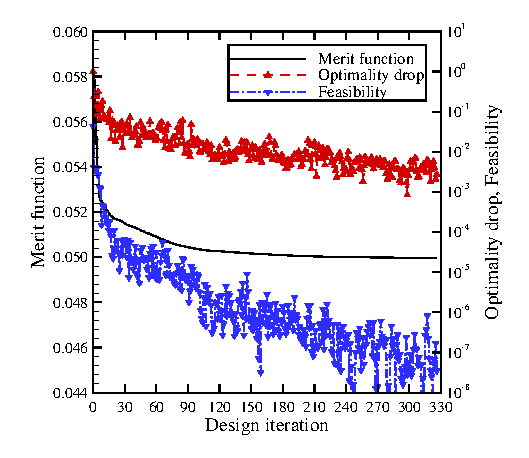
\includegraphics[width=4.5in]{Figures/No_Twist/A320neo/Optimize_A320_Fixed_Orig_No_Twist.eps}
\caption{Convergence history for A320neo optimization without wing twist with a sweep angle limit at the original sweep angle of 27.9\degree.}
\label{fig:a320neo_notwist_converge_baseline}
\end{figure}

\begin{figure}[!tp]
\centering
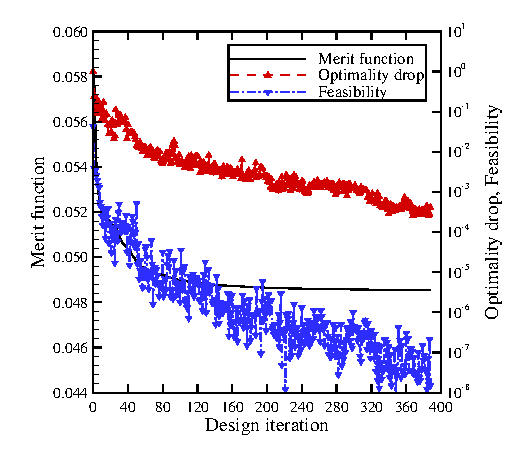
\includegraphics[width=4.5in]{Figures/No_Twist/A320neo/Optimize_A320_No_Twist_60deg.eps}
\caption{Convergence history for A320neo optimization without wing twist with an upper sweep angle limit of 60.0\degree.}
\label{fig:a320neo_notwist_converge_60.0_Deg}
\end{figure}

%%%%%% A320neo NO TWIST RESULTS TABLE %%%%%%
\begin{table}[!tp]
\centering
\caption{Results summary for the optimization of the A320neo without wing twist}
\label{tab:a320neo_notwist_results}
\begin{adjustbox}{center}
\begin{tabular}{lcccc}
\hline\hline
Design Variable & Trimmed Baseline & Original (27.9\degree)\ Sweep Limit & 60.0\degree\ Sweep Limit\\
\hline
$S$ (ref. units\textsuperscript{2}) & 3.340 & 3.340 & 3.340 \\
$C_L S$ & 1.669 & 1.667 & 1.667 \\
$C_M S$ & -0.736 & -0.752 & -2.268 \\
$C_D S$ (counts) & 598.2 & 499.7 & 485.6 \\
$L/D$ & 27.89 & 33.39 & 34.37 \\
Angle of Attack & 2.303\degree\ & 1.655\degree\ & 2.238\degree\ \\
\makecell[l]{Post-Optimization\\Leading Edge Sweep Angle} & 27.9\degree\ & 27.89\degree\ & 46.67\degree\ \\
\hline\hline
\end{tabular}
\end{adjustbox}
\end{table}

Plots of the pressure contours on the upper surface of the A320neo ASOs without wing twist are shown in Figure~\ref{fig:a320neo_notwist_planform_plots}. Plots of the section shape and pressure distribution at numerous spanwise sections are presented in Figure~\ref{fig:a320neo_notwist_section_plots}, which include the trimmed angle of attack baseline, the fixed-sweep ASO at the original sweep angle of 27.9\degree\ and the 60.0\degree\ sweep limit ASO.

%%%%%% A320neo NO TWIST PLANFORM PLOTS %%%%%%
\begin{figure}[!tp]
    \centering
    \subfloat[\label{fig:a320neo_notwist_opt_baseline_planform}]{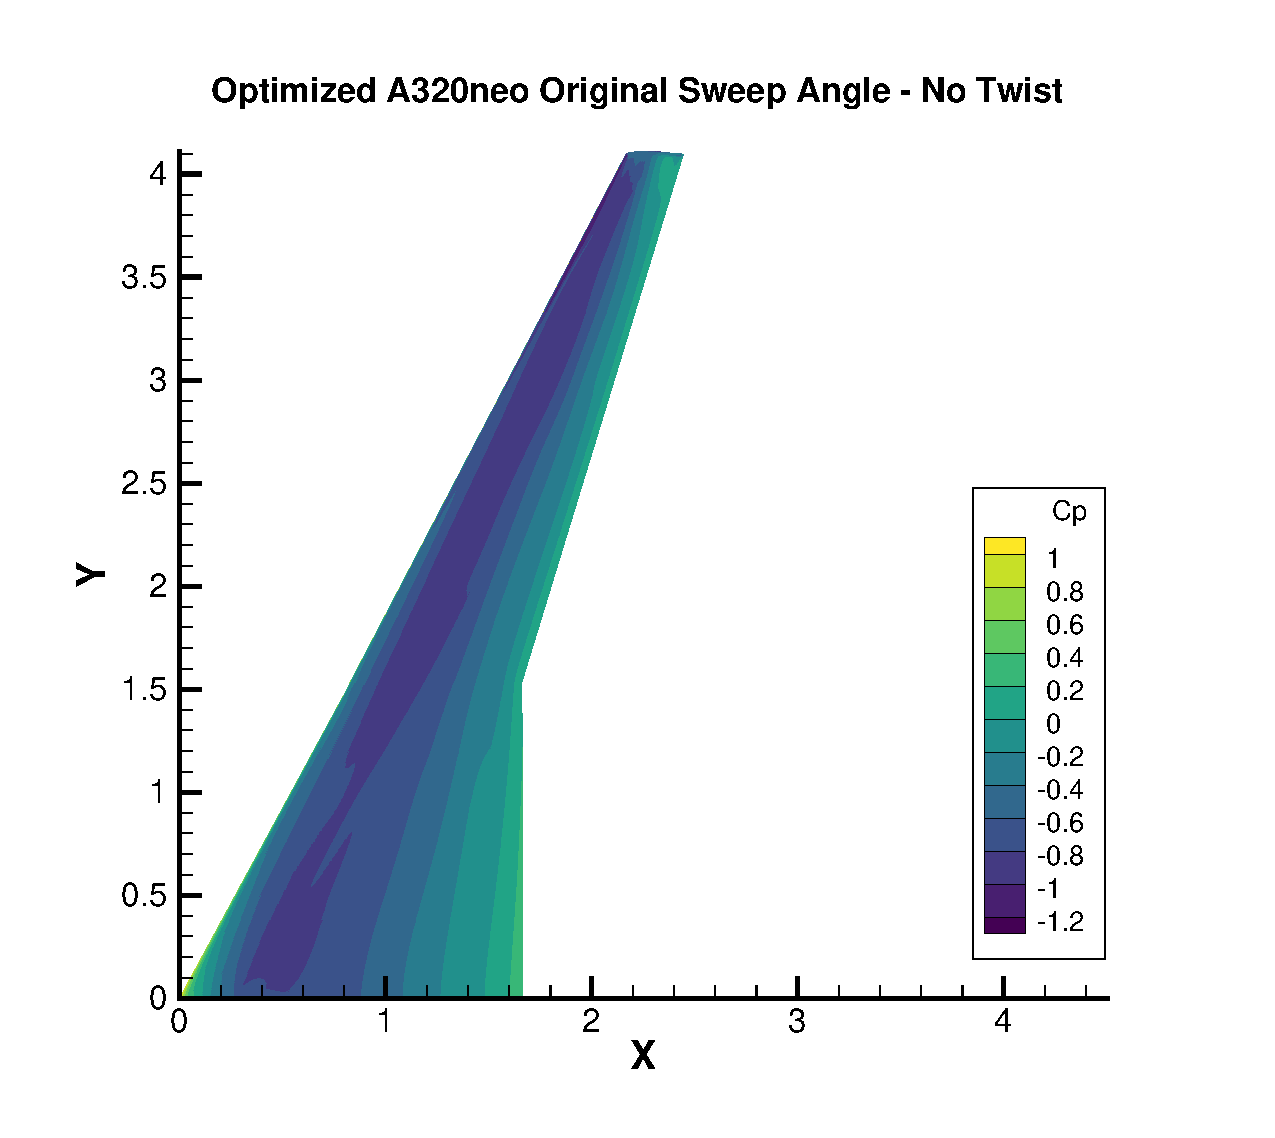
\includegraphics[trim={0.25cm 0.25cm 0.25cm 0.25cm},clip,width=3.175in]{Figures/No_Twist/A320neo/A320_Fixed_Orig_No_Twist-Contour-Upper.eps}}
    \hspace{0.25cm}
    \subfloat[\label{fig:a320neo_notwist_60_deg_planform}]{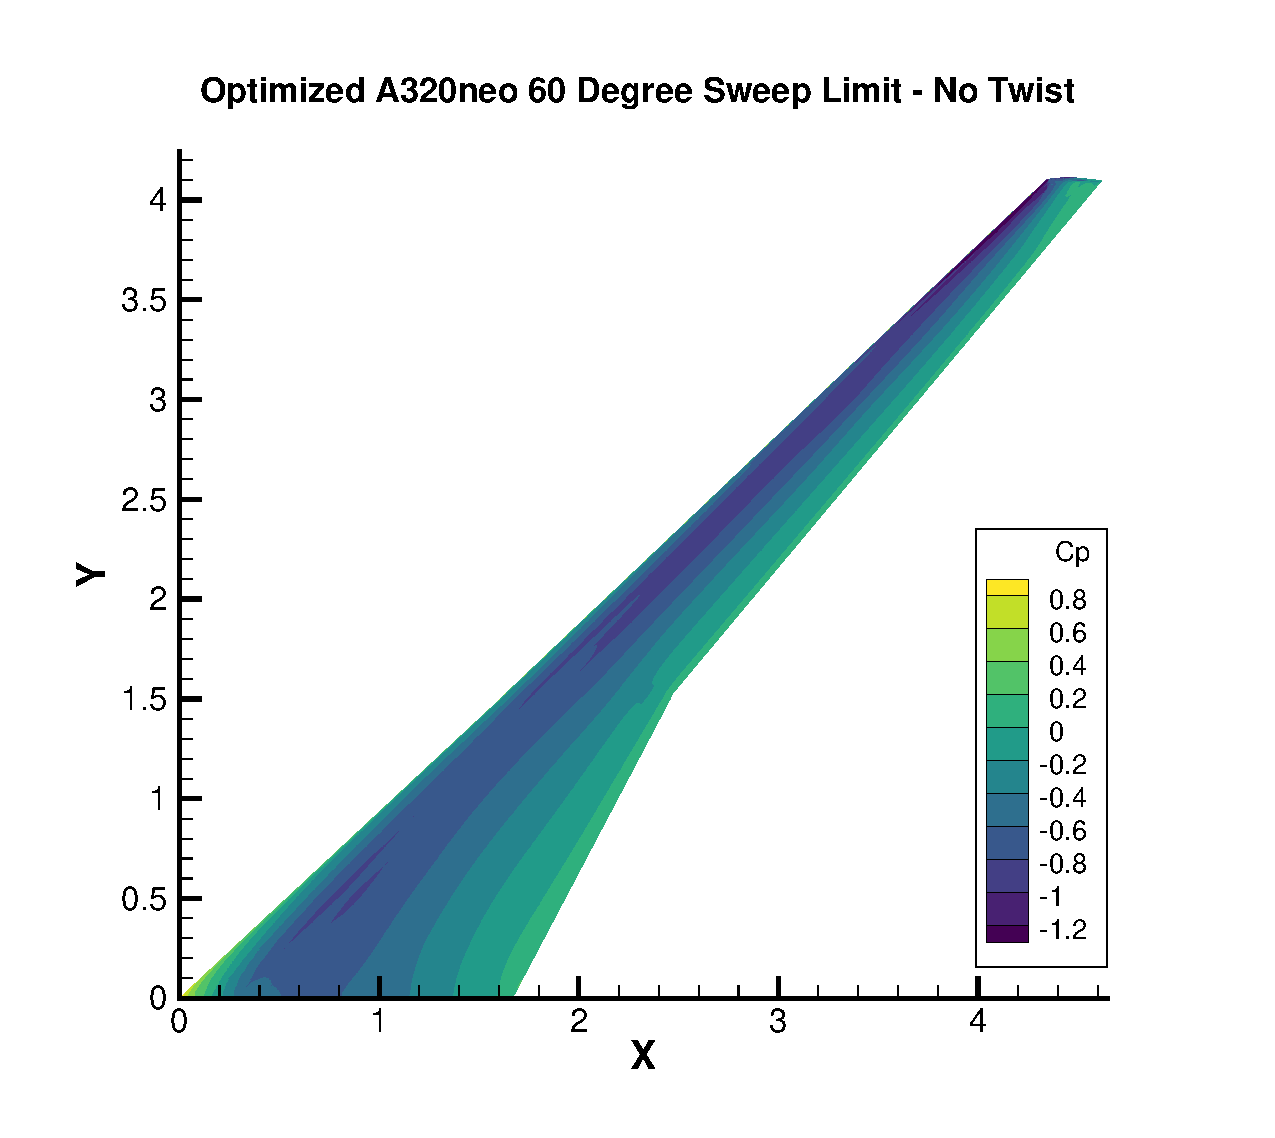
\includegraphics[trim={0.25cm 0.25cm 0.25cm 0.25cm},clip,width=3.175in]{Figures/No_Twist/A320neo/A320neo_varsweep_NoTwist_60deg-Contour-Upper.eps}}
    \caption{A320neo upper surface pressure contours for the original sweep angle limit optimized planform (\ref{fig:a320neo_notwist_opt_baseline_planform}) and 60.0\degree\ sweep angle limit optimized planform (\ref{fig:a320neo_notwist_60_deg_planform}) without wing twist in optimization.}
\label{fig:a320neo_notwist_planform_plots}
\end{figure}
\FloatBarrier

%%%%%% A320neo NO TWIST SECTION PLOTS %%%%%%
\begin{figure}[!tp]
    \centering
    \subfloat[\label{fig:a320neo_notwist_section_1_perc}]{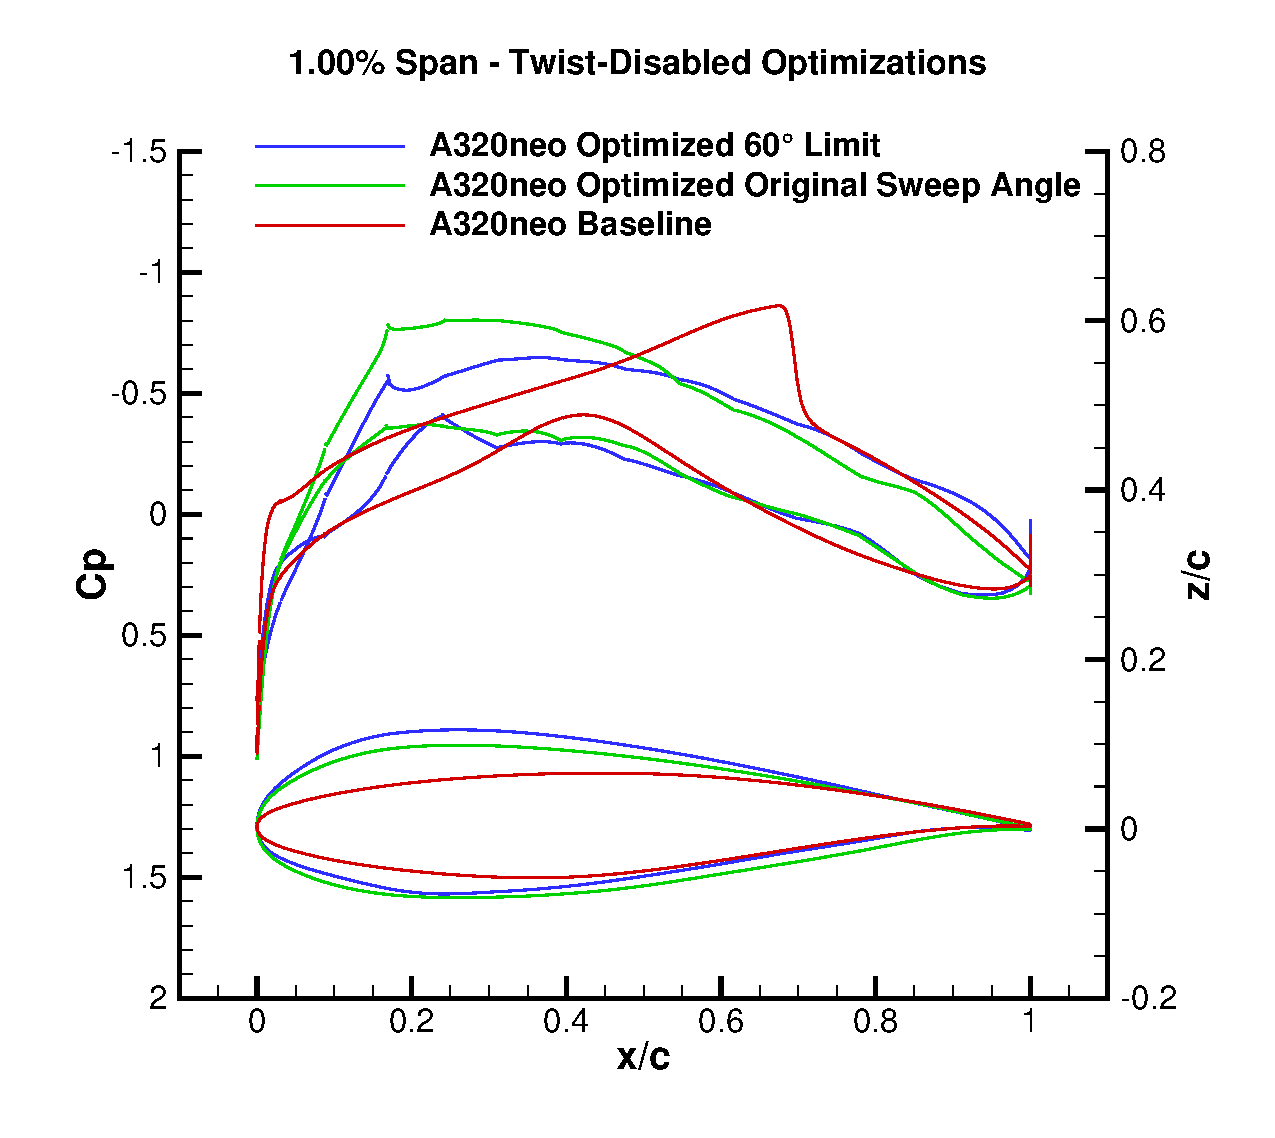
\includegraphics[trim={0.25cm 0.25cm 0.25cm 0.25cm},clip,width=3in]{Figures/No_Twist/A320neo/A320neo_Optimize_NoTwist-1.00percent_Span.eps}}
    \hspace{0.25cm}
    \subfloat[\label{fig:a320neo_notwist_section_20.6_perc}]{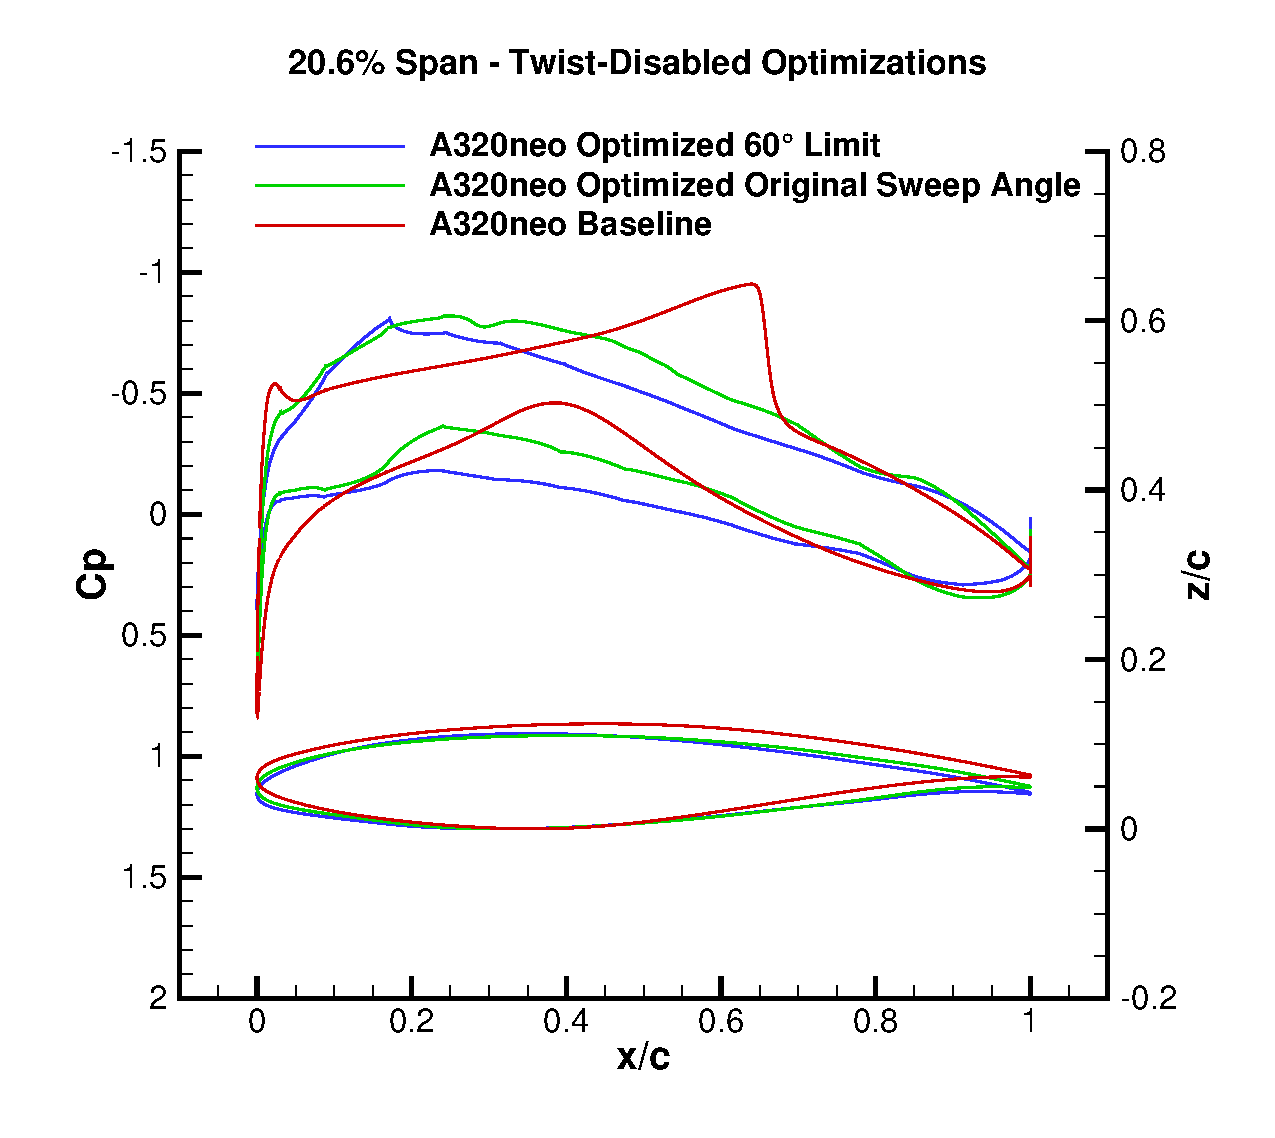
\includegraphics[trim={0.25cm 0.25cm 0.25cm 0.25cm},clip,width=3in]{Figures/No_Twist/A320neo/A320neo_Optimize_NoTwist-20.6percent_Span.eps}}\\
    \subfloat[\label{fig:a320neo_notwist_section_40.2_perc}]{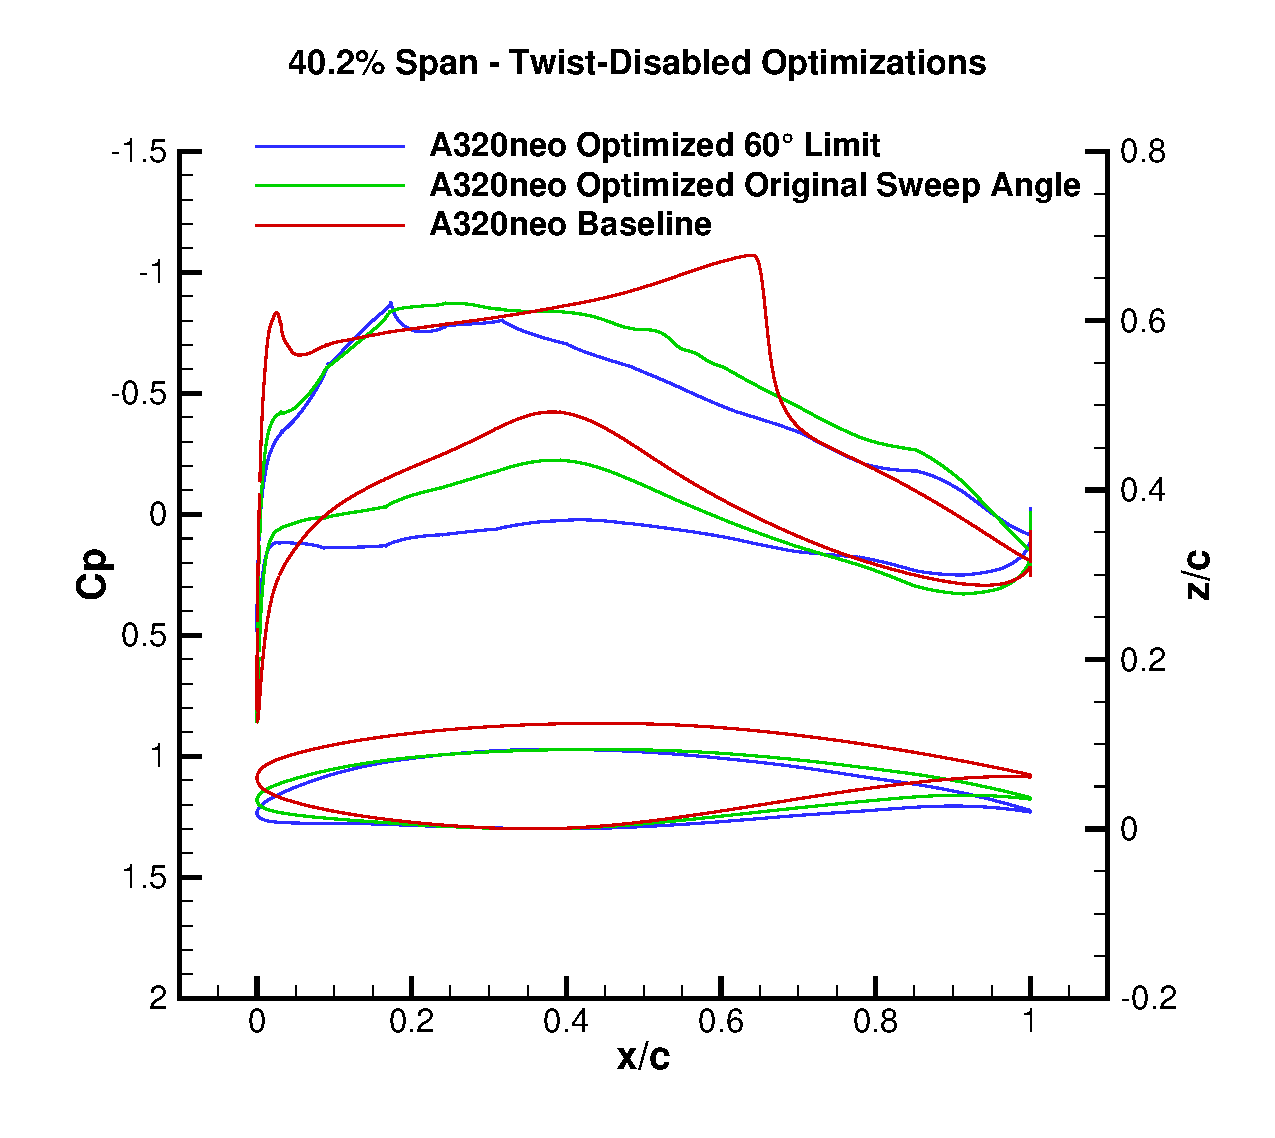
\includegraphics[trim={0.25cm 0.25cm 0.25cm 0.25cm},clip,width=3in]{Figures/No_Twist/A320neo/A320neo_Optimize_NoTwist-40.2percent_Span.eps}}
    \hspace{0.25cm}
    \subfloat[\label{fig:a320neo_notwist_section_59.8_perc}]{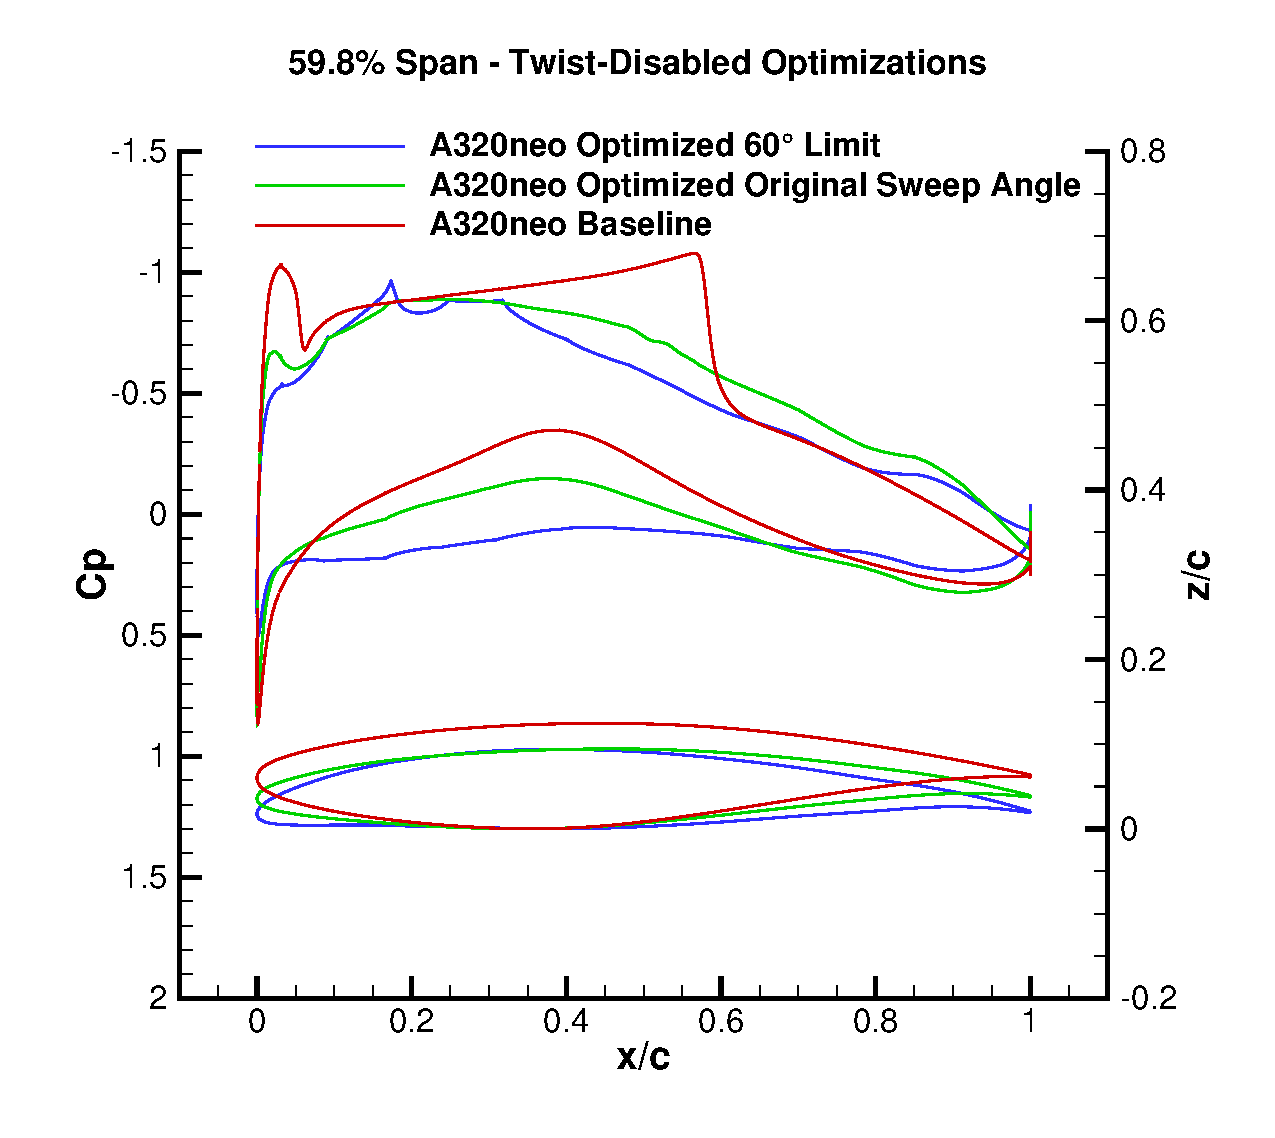
\includegraphics[trim={0.25cm 0.25cm 0.25cm 0.25cm},clip,width=3in]{Figures/No_Twist/A320neo/A320neo_Optimize_NoTwist-59.8percent_Span.eps}}\\
    \subfloat[\label{fig:a320neo_notwist_section_79.4_perc}]{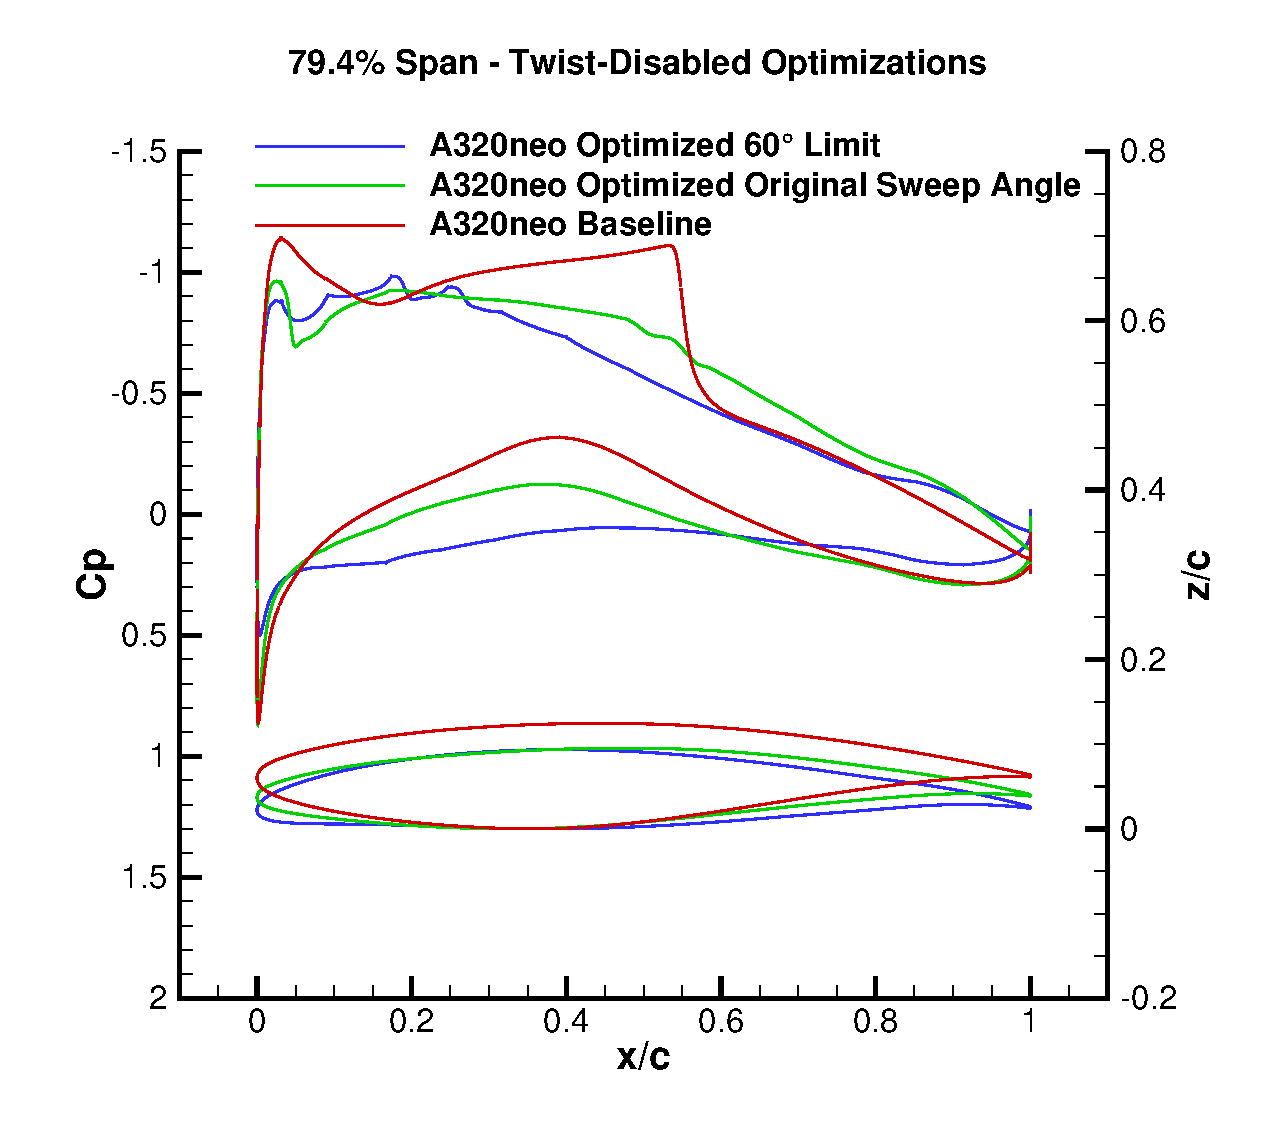
\includegraphics[trim={0.25cm 0.25cm 0.25cm 0.25cm},clip,width=3in]{Figures/No_Twist/A320neo/A320neo_Optimize_NoTwist-79.4percent_Span.eps}}
    \hspace{0.25cm}
    \subfloat[\label{fig:a320neo_notwist_section_99.0_perc}]{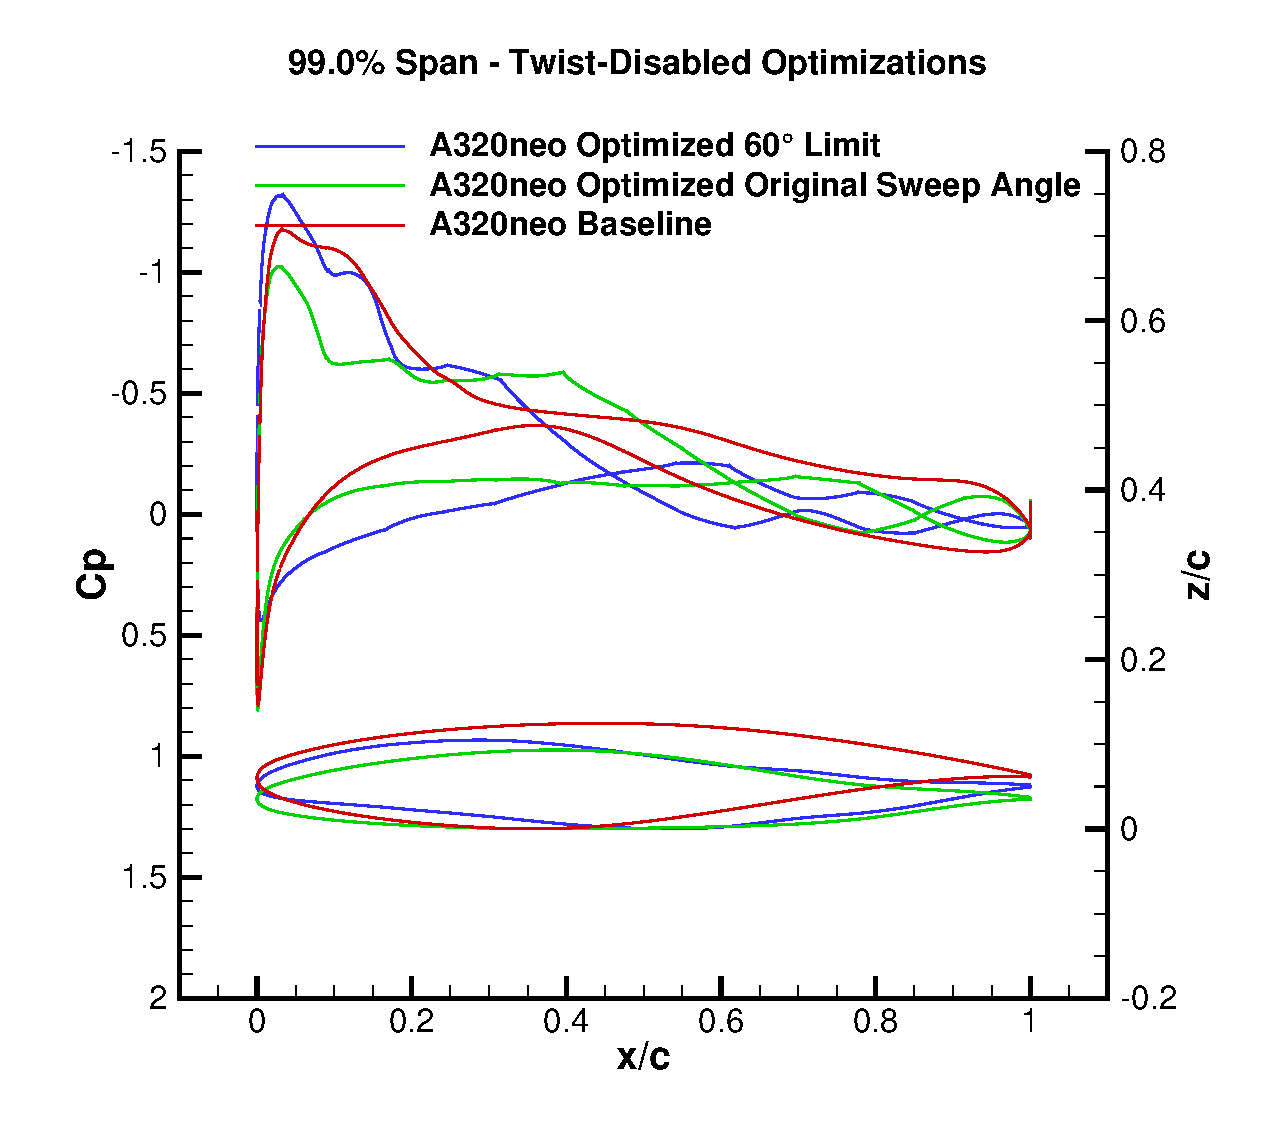
\includegraphics[trim={0.25cm 0.25cm 0.25cm 0.25cm},clip,width=3in]{Figures/No_Twist/A320neo/A320neo_Optimize_NoTwist-99.0percent_Span.eps}}
    \caption{Section geometry and pressure distribution plots of the trimmed angle of attack A320neo baseline planform and 60.0\degree\ sweep angle limit optimized planform at 1.00\% (\ref{fig:a320neo_notwist_section_1_perc}), 20.6\% (\ref{fig:a320neo_notwist_section_20.6_perc}), 40.2\% (\ref{fig:a320neo_notwist_section_40.2_perc}), 59.8\% (\ref{fig:a320neo_notwist_section_59.8_perc}), 79.4\%(\ref{fig:a320neo_notwist_section_79.4_perc}), and 99.0\% (\ref{fig:a320neo_notwist_section_99.0_perc}) span.}
\label{fig:a320neo_notwist_section_plots}
\end{figure}
\FloatBarrier

The A320neo ASO cases without wing twist are able to eliminate the sharp drop in pressure that occurs between 60-80\% of the local chord on the upper surface of the wing in Figure~\ref{fig:a320neo_section_plots}. This is especially notable in the fixed sweep angle optimization at 27.9\degree, which achieves this without any increase to the sweep angle. The absence of a shock on the optimized wings suggests that the wave drag has been eliminated.

Compared to the NASA CRM cases without wing twist, the A320neo cases do not possess as smooth of a pressure recovery. The leading edge of the wing exhibits many perturbations in the pressure coefficient as it approaches peak suction over the upper surface. The pressure recovery is also not nearly as smooth as that exhibited in the CRM twist-deactivated cases. However, both A320neo cases without twist are able to eliminate the adverse pressure gradient that is observed on the leading half of the airfoil in the trimmed baseline case, and have achieved a favourable pressure gradient past 20\% of the local chord.

Comparing between the 60.0\degree\ sweep limit case without twist and the fixed sweep angle optimization at 27.9\degree\ shows that the latter case achieves many of the performance characteristics of the former without an increase in the wing's sweep angle. Nevertheless, the pressure recovery for the optimized planform at the original sweep angle of 27.9\degree\ is not as smooth, with many small pressure perturbations over the upper surface of the wing past 40\% local chord along the entire wingspan, although it is unclear why this has occurred.

The section shapes for both the 27.9\degree\ fixed sweep angle and 60.0\degree\ sweep limit optimizations are very similar, which mirrors the behaviour observed in the the previous A320neo ASO cases, as well as the CRM ASO cases without wing sweep. The root section shape is substantially thicker for both optimized wings compared to the initial geometry, as seen in Figure~\ref{fig:a320neo_notwist_section_1_perc}. The thickness decreases along the remainder of the wingspan to become thinner than the initial geometry. This result agrees well with the results of other studies~\cite{ledoux_study_2015, kenway_multipoint_2015, telidetzki_application_2014, lyu_rans-based_2014, lyu_aerodynamic_2015, osusky_drag_2015, shi-dong_approximate_2018, yu_influence_2018, koo_investigation_2018}, as the minimum volume constraint incites this behaviour so as to create a thin outboard wing. 
% The section shape between the root and outboard section differs dramatically compared to the A320neo ASO cases with twist. When twist is disabled, the mid-wing section shape becomes substantially thinner, with both the leading and trailing edge dropping down while the upper and lower section between 20-60\% local chord flattens out.
The mid-chord sections reduces are flattened, while the leading and trailing edge have been lowered. This trailing edge does not appear to have lowered as much as the leading edge, giving the appearance that the local twist on the wing has changed. This behaviour suggests that the optimizer is attempting to modify the local twist on the wing without violating the twist equality constraint of 0\degree. Similar behaviour appeared in the CRM ASO cases without wing twist.

Yet again, the strange behaviour is exhibited at the wingtip. In both the 27.9\degree\ sweep angle and 60.0\degree\ sweep limit cases without wing twist, the optimizer has produced a section shape with a reflexed camber line, as seen in Figure~\ref{fig:a320neo_notwist_section_99.0_perc}. 
% Positive camber is exhibited before 50\% local chord, while negative camber is exhibited aft of it. This behaviour was demonstrated in all other optimization cases for both the A320neo and the NASA CRM. 
Since changes to wing twist were not permitted in these 27.9\degree\ sweep angle and 60.0\degree\ sweep limit cases, it appears that this behaviour must result from other design variables. It is unclear what the origin of this behaviour is, and a thorough search of relevant literature did not produce any studies with similar results.

The results of the ASO on the A320neo at a fixed sweep angle of 27.9\degree\ and a sweep limit of 60.0\degree\ without wing twist are not directly comparable to other studies. A search of relevant literature did not produce ASO studies on the A320neo on a similar basis to this study. Therefore, these results stand alone as novel results at the time of writing. 

\section{Drag Behavior with Varying Sweep Angles}
\label{sec:crm-drag-trends}
%%%%%%%%%%%%% TALK ABOUT DISCRETE ANGLE STUDY HERE %%%%%%%%%%%%%
The characterization of the aircraft drag as a function of the sweep angle was conducted as described in section~\ref{sssec:drag-opt-methods}. The ASO on the CRM wing was conducted at fixed sweep angles with local wing twist disabled, but with angle of attack and section shape included. The disabling of local wing twist as a design variable corresponds to a local twist equality constraint of 0\degree. This choice of design variables was made in consideration of the geometry artifacts on the CRM wing that are produced when local twist changes are permitted, as in section~\ref{ssec:crm-opt-twist}. The ASO case without wing twist at the original sweep angle of 37.5\degree\ is identical to that conducted in section~\ref{ssec:crm-opt-notwist}, such that it will be reused here. The trimmed baseline case presented in section~\ref{ssec:crm-opt-twist} and the 60.0\degree\ sweep limit case without wing twist in section~\ref{ssec:crm-opt-notwist} were also used for comparison in this study. The resultant parameters for the remaining cases to be run at fixed sweep angles of 40.0\degree\ and 42.5\degree\ are presented in Table~\ref{tab:crm_drag_trend_study}, with all other parameters remaining unchanged as presented in Table~\ref{tab:crm-opt}.

Both the 40.0\degree\ and 42.5\degree\ fixed-sweep angle CRM ASO cases converged very smoothly. Qualitative analysis of the merit function, optimality, and feasibility demonstrated that the 40.0\degree\ case converged after 330 design iterations, whereas the 42.5\degree\ case converged after 288 design iterations, as seen in Figures~\ref{fig:crm_notwist_converge_40.0_Deg} and~\ref{fig:crm_notwist_converge_42.5_Deg}, respectively. The 40.0\degree\ case exhibited a decrease in the drag coefficient $C_D S$ by 55 drag counts compared to the trimmed baseline, but only decreased by 2.5 drag counts compared to the ASO at the original (37.5\degree) sweep angle, as seen in Table~\ref{tab:crm_drag_trend_results}. The angle of attack increased by 2.4\degree\ to 39.90\degree\ compared to the trimmed baseline planform, and by approximately 2.6\degree\ relative to the 37.5\degree\ ASO case. The moment coefficient $C_M S$ decreased moderately by 0.227 to -2.931 compared to the trimmed baseline planform, and by 0.214 compared to the 37.5\degree\ ASO case. The $L/D$ increased by almost 3 counts compared to the trimmed baseline planform, but only increased by 0.15 compared to the ASO at the original sweep angle. The 40.0\degree\ case performed 9.316\% better relative to the trimmed baseline and 0.460\% better relative to the optimization at the original sweep angle, using the drag coefficient as the basis of comparison.

\begin{table}[!tp]
\centering
\caption{Modified design variable constraints for CRM 40.0\degree\ and 42.5\degree\ drag behaviour study optimization cases.}
\label{tab:crm_drag_trend_study}
\begin{tabular}{lrrrr}
\hline\hline
Constraint & \multicolumn{2}{c}{40.0\degree\ Fixed Sweep Angle} & \multicolumn{2}{c}{42.5\degree Fixed Sweep Angle}\\ \hline
 & \multicolumn{1}{c}{Lower Limit} & \multicolumn{1}{c}{Upper Limit} & \multicolumn{1}{c}{Lower Limit} & \multicolumn{1}{c}{Upper Limit}\\ \hline
Local Twist & 0\degree & 0\degree & 0\degree & 0\degree \\
Leading Edge Sweep Angle & 40.0\degree & 40.0\degree & 42.5\degree & 42.5\degree \\ \hline\hline
\end{tabular}
\end{table}


%%%%%% CRM NO TWIST DRAG TREND CONVERGENCE PLOTS %%%%%%
\begin{figure}[!tp]
\centering
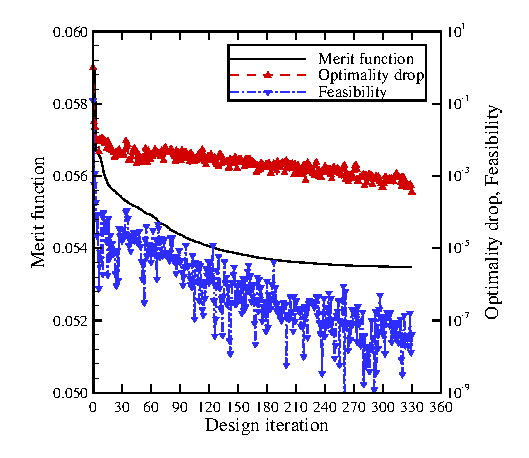
\includegraphics[width=4.5in]{Figures/No_Twist/NASA_CRM/Optimize_CRM_FIXED_No_Twist_40.0deg.eps}
\caption{Convergence history for NASA-CRM optimization without wing twist and an upper sweep angle limit of 40.0\degree.}
\label{fig:crm_notwist_converge_40.0_Deg}
\end{figure}

\begin{figure}[!tp]
\centering
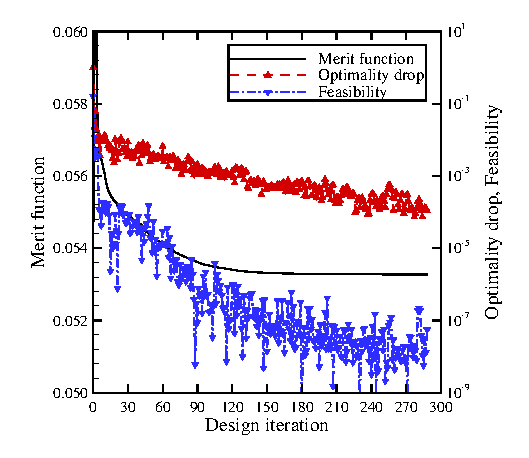
\includegraphics[width=4.5in]{Figures/No_Twist/NASA_CRM/Optimize_CRM_FIXED_No_Twist_42.5deg.eps}
\caption{Convergence history for NASA-CRM optimization without wing twist and an upper sweep angle limit of 42.5\degree.}
\label{fig:crm_notwist_converge_42.5_Deg}
\end{figure}

%%%%%%% TABLE OF RESULTS %%%%%%%
\begin{table}[!tp]
\centering
\caption{Results summary for the optimization of the NASA CRM without wing twist at varying wing sweep angles}
\label{tab:crm_drag_trend_results}
\begin{adjustbox}{center}
\begin{tabular}{lccccc}
\hline\hline
Design Variable & Trimmed Baseline & \makecell{Original (37.5\degree)\\Sweep Angle} & \makecell{40.0\degree\\Sweep Angle} & \makecell{42.5\degree\\Sweep Angle} & \makecell{60.0\degree\\Sweep Limit}\\
\hline
$S$ (ref. units\textsuperscript{2}) & 3.395 & 3.394 & 3.394 & 3.393 & 3.393\\
$C_L S$ & 1.6972 & 1.6972 & 1.6972 & 1.6972 & 1.6972\\
$C_M S$ & -2.704 & -2.717 & -2.931 & -3.148 & -3.742 \\
$C_D S$ (counts) & 589.7 & 537.2 & 534.7 & 532.7 & 531.1\\
$L/D$ & 28.78 & 31.59 & 31.74 & 31.86 & 31.96\\
Angle of Attack & 1.982\degree & 1.771\degree & 1.802\degree & 1.904\degree & 2.225\degree \\[0.25cm]
\makecell[l]{Post-Optimization\\Leading Edge Sweep Angle} & 37.50\degree & 37.31\degree & 39.90\degree & 42.40\degree & 48.50\degree \\[0.5cm]
\makecell[l]{Change in $C_D S$\\Relative to Trimmed Baseline} & 0.000\% & -8.897\% & -9.316\% & -9.663\% & -9.936\% \\[0.5cm]
\makecell[l]{Change in $C_D S$\\Relative to Optimization at\\Original (37.5\degree) Sweep Angle} & 11.03\% & 0.000\% & -0.460\% & -0.841\% & -1.141\% \\
\hline\hline
\end{tabular}
\end{adjustbox}
\end{table}

The 42.5\degree\ sweep angle ASO case displayed an almost linear improvement over the 40.0\degree\ case, relative to the optimization at the original sweep angle. The drag coefficient decreased by 57 drag counts compared to the trimmed baseline and decreased by 4.5 drag counts compared to the ASO at the original (37.5\degree) sweep angle. The angle of attack increased by 4.9\degree\ over the trimmed baseline and by 5.1\degree\ over the optimization at 37.5\degree. The moment coefficient decreased further, decreasing by 0.444 and 0.431 relative to the trimmed baseline and 37.5\degree\ case, respectively. The $L/D$ increased by just over 3 and 0.1 counts relative to the trimmed baseline and 37.5\degree\ case, respectively. The 42.5\degree\ case performed 9.663\% better relative to the trimmed baseline and 0.841\% better relative to the optimization at the original sweep angle, using the drag coefficient as the basis of comparison. The changes in almost all performance metrics represents a sub-linear increase in performance, and is very nearly linear.

Plots of the changes in the drag coefficient $C_D S$ by drag count for the trimmed baseline, optimized cases at fixed sweep angles, and the 60.0\degree\ sweep limit cases are given in Figure~\ref{fig:crm_drag_trend_abs}. The change in drag coefficient relative to the trimmed baseline CRM wing is given in Figure~\ref{fig:crm_drag_trend_perc_baseline}, which illustrates that the biggest performance improvements are obtained without having to include wing sweep as a design variable, wherein an 8.9\% reduction in drag is obtained. Using the wing optimized at the original sweep angle as the basis of comparison places the results into context, wherein one can clearly see the almost linear benefits in drag reduction for initial increases in the sweep angle in Figure~\ref{fig:crm_drag_trend_perc_opt_baseline}. Calculating the rate of change in drag between the 37.5\degree\ and 40.0\degree\ optimization results produces a 0.18\% decrease in drag per 1\degree\ increase in sweep, or a decrease in 1 drag count per degree.

This slope decreases with further increases in sweep, evidenced by the -0.15\% per degree decrease in drag obtained between the 40.0\degree\ and 42.5\degree\ optimized wings. The slope continues to decrease between the 42.5\degree\ sweep angle and 60.0\degree\ sweep limit cases, the latter of which produces 48.50\degree\ sweep angle wing. The rate of change of drag in this section is -0.120\% per degree, which is far lower than the slope at the initial sweep angle changes.


% Drag trend plot
\begin{figure}[!tp]
\centering
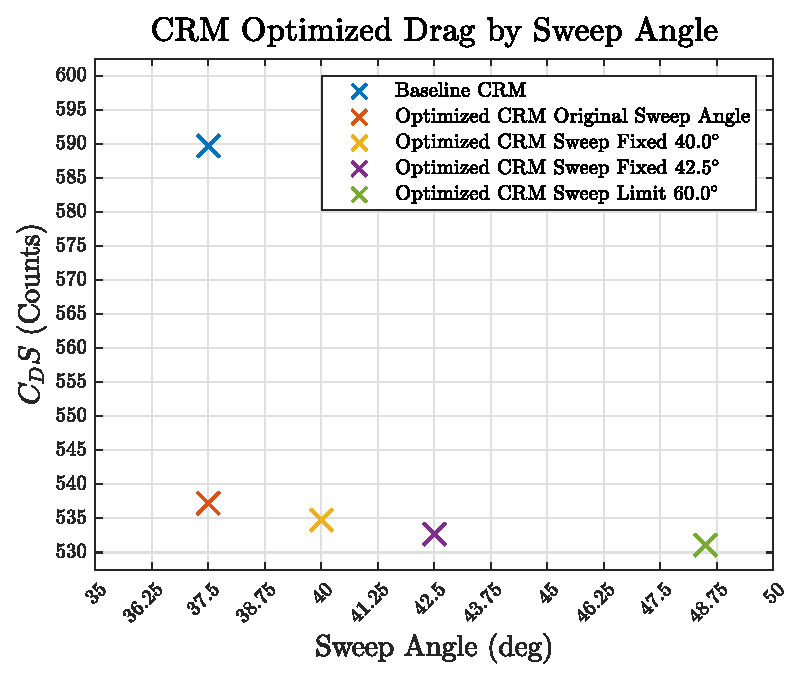
\includegraphics[width=4.5in]{Figures/Drag_Trend/crm_drag_trend.eps}
\caption{Plot of $C_{D} S$ by sweep angle for baseline, fixed sweep angle [37.5, 40.0, 42.5], and varying sweep angle (60.0\degree\ limit) optimization cases.}
\label{fig:crm_drag_trend_abs}
\end{figure}

\begin{figure}[!tp]
\centering
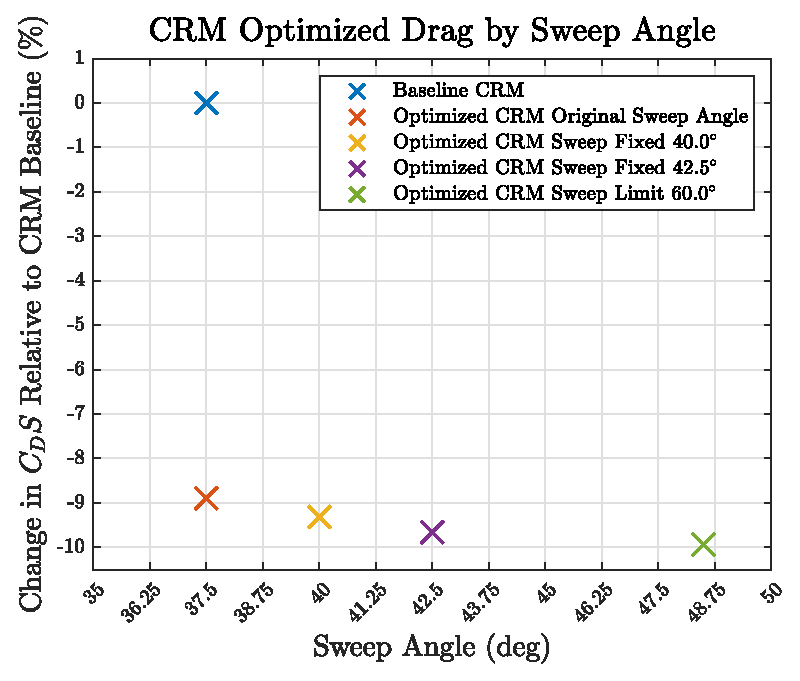
\includegraphics[width=4.5in]{Figures/Drag_Trend/crm_drag_trend_perc.eps}
\caption{Plot of percent change in $C_{D} S$ by sweep angle relative to baseline CRM configuration for trimmed baseline, fixed sweep angle [37.5, 40.0, 42.5], and varying sweep angle (60.0\degree\ limit) optimization cases.}
\label{fig:crm_drag_trend_perc_baseline}
\end{figure}

\begin{figure}[!tp]
\centering
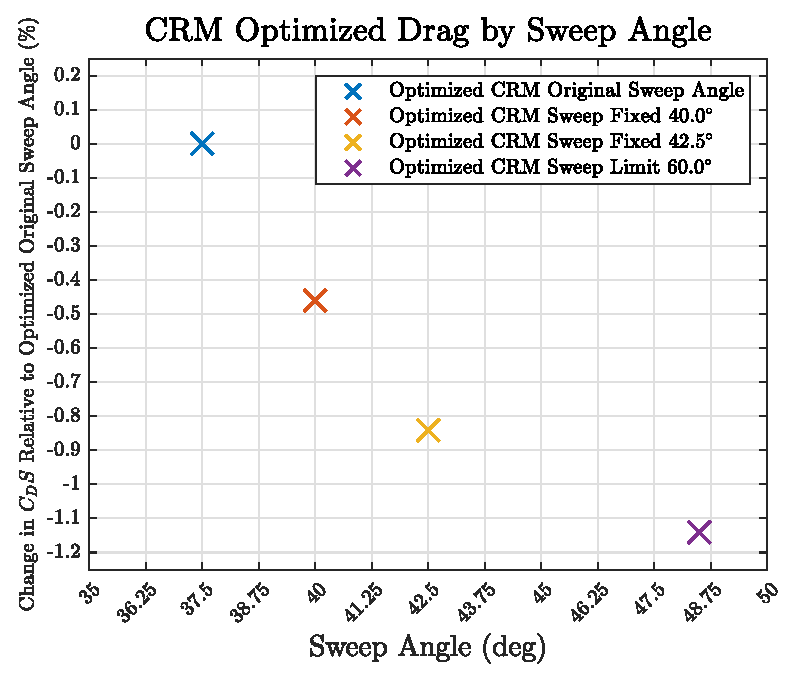
\includegraphics[width=4.5in]{Figures/Drag_Trend/crm_drag_trend_perc_2.eps}
\caption{Plot of percent change in $C_{D} S$ by sweep angle relative to CRM optimized at original sweep angle for fixed sweep angle [37.5, 40.0, 42.5] and varying sweep angle (60.0\degree\ limit) optimization cases.}
\label{fig:crm_drag_trend_perc_opt_baseline}
\end{figure}
\FloatBarrier
    \chapter{Discussion}
\section{Multidisciplinary Considerations}
The original intention of this study was to answer a single question: when sweep is included as a design variable in pure ASO, at what point will the wing sweep angle stop growing, if at all? This was answered through both the CRM and A320neo optimizations, where the former's wing sweep angle reaches an optimum at 48.50\degree\ without wing twist, and the latter's reaches an optimum at 46.70\degree. The drag benefits over the trimmed baseline cases for both wings are substantial, up to 9.936\% for the CRM wing and 18.824\% for the A320neo. Yet, these results are actually quite nuanced. While an improvement over the baseline is quite productive towards improvements in efficiency and aircraft sustainability, a secondary question is one of whether increasing the sweep angle is actually necessary to yield such performance improvements. Optimizations at the original sweep angles of the CRM and A320neo wings were conducted and compared to the results at the optimal sweep angles, illustrating that the real performance benefits of adding sweep are much smaller than how they initially appear. For the CRM, this benefit was only 1.141\% over the original sweep angle while for the A320neo it was slightly greater, at 2.827\%. This indicates that the design space appears to be quite flat with respect to an aircraft's sweep angle, and that the benefits may be less significant compared to the magnitude of numerical error as one approaches the optimal sweep angle.

The NASA CRM and A320neo comparison to the optimizations at their original sweep angles further emphasizes the question of whether substantial changes to sweep are truly worthwhile. Indeed, increasing the sweep angle of an aircraft is actually quite a substantial change with cascading effects. It produces differences in the centre of gravity and lift of the aircraft, changing its moment and consequently, its stability characteristics. Without a change to the position of the wing along the length of the fuselage, this would require a change in the trimmed configuration of the aircraft with respect to the elevons and their trim tabs. The increased trim force required to counteract an increased moment may partially or even completely negate the benefits obtained by increasing the sweep, especially when the benefits are compared to an optimization at the original sweep angle, relative to which the drag benefits of increasing sweep are much lower. Operational design factors would be impacted as well. Constraints on certain wing design parameters are influenced by airport gate and service equipment requirements, such that an aircraft with a substantially increased sweep may not be able to park at a gate or serviced by airport vehicles due the risk of collision when the wings are at a greater sweep angle.

 The impact on the structural design of the wing is considerably affected by changes in the sweep angle as well. An increased sweep angle on an aircraft increases the bending moment and torsional loads along the wing and at its joint with the fuselage. Therefore, an increase an aircraft's wing sweep comes with a structural weight penalty in order for the design to be structurally feasible. Moreover, an increase in weight cascades back to aerodynamic performance, as the induced drag on an aircraft is proportional to the weight of the aircraft squared, which is derived from the lift and induced drag coefficients of an aircraft. Furthermore, it is known that the induced drag on an aircraft is approximately half of the total drag. Therefore, for a given change in sweep to be beneficial, the wing's drag must be reduced by a greater percentage than the increase in the wing weight.
\begin{equation}
~\label{eqn:lift_coef}
    C_L = \frac{L}{\frac{1}{2}\rho_0 V_{E}^2 S}
\end{equation}
\begin{equation}
~\label{eqn:induced_drag}
    \begin{split}
        C_{D,i} = \frac{C_{L}^2}{\pi\frac{b^2}{S}e}
    \end{split}
\end{equation}\par
An estimate of the wing weight as a result of changes in the wing sweep angle may be calculated using Equation~\ref{eqn:wing_weight},
\begin{equation}
~\label{eqn:wing_weight}
W_{wing}=W_G k_w b_{s}^{0.75} \left[1+\sqrt{\frac{b_{\text{ref}}}{b_s}}\right] n_{\text{ult}}^{0.55} \left[\frac{b_s/t_r}{W_G /S}\right]
\end{equation}
which is a modified version of that presented by Kuntawala~\cite{kuntawala_aerodynamic_2011}. In this equation, $W_G \text{lb} = MZFW = \text{gross weight}$; $k_w = 1.7\times10^-3$; $b_s=b/\cos{\Lambda}=\text{structural span}$ where $b = \text{wing span (ft)}$, $\Lambda = \text{sweepback angle at the leading edge (deg)}$; $b_{\text{ref}}=6.25\text{ft}=\text{reference span}$; $n_{\text{ult}}=\text{ultimate load factor}$; $t_r=\ $(absolute) maximum thickness of root chord (ft); and $S=\text{(projected) area of the wing (ft^2)}$.

The approximate total aircraft cruise weight is calculated for each aircraft and assumes that the total aircraft fuel weight $(W_F)$ is found by $W_F=MTOW-MZFW$, and that the fuel weight at cruise is 85\% of the total fuel weight. The total aircraft cruise weight is calculated as in Equation~\ref{eqn:cruise_weight}.
\begin{equation}
~\label{eqn:cruise_weight}
    W_{\text{cruise}}=0.85\times W_F+MZFW
\end{equation}\par
The NASA CRM configuration is similar to the Boeing 777-200ER, such that its design weights may be used to approximate the CRM's cruise weight and gross weight. Kenway et al.~\cite{kenway_aerostructural_2014} summarize these design weights, resulting in $W_{\text{cruise}}=593,193\ \text{lb}$ and $W_G=429,990\ \text{lb}$ for the CRM in its original configuration. 

Chau and Zingg~\cite{chau_aerodynamic_2023} present the A320neo's design weights, resulting in $W_{\text{cruise}}=169,452\ \text{lb}$ and $W_G=142,090\ \text{lb}$ for the A320neo in its original configuration. Chau and Zingg also present the A320neo's wing weight, allowing for a benchmark of Equation~\ref{eqn:wing_weight} using the A320neo's actual wing weight. Equation~\ref{eqn:wing_weight} produces a wing weight of $18,682\ \text{lb}$ for the A320neo in its original configuration, compared to the A320neo's real wing weight of $18,710\ \text{lb}$. This is a difference of 0.150\%, which is considered to be tolerable in this study.

The wing weights by sweep angle, percent change in wing weight, percent change in total aircraft cruise weight, and percent change in total aircraft drag for the CRM results presented in section~\ref{sec:crm-drag-trends} are given in Table~\ref{tab:crm_weight_results}. It must be noted that the optimization at the original sweep angle was measured to have decreased in sweep angle by 0.2\degree. This is considered a numerical error for the sake of weight calculations, as it would otherwise decrease the weight of this wing. Hence, weight comparisons are made with respect to the original configuration studied in the "trimmed baseline" case.

%%%%%%% TABLE OF WEIGHTS %%%%%%%
\begin{table}[!tp]
\centering
\caption{Weight and drag trade-off results for the optimization of the NASA CRM without wing twist}
\label{tab:crm_weight_results}
\begin{adjustbox}{center}
\begin{tabular}{lccccc}
\hline\hline
Variable & Trimmed Baseline & \makecell{Original (37.5\degree)\\Sweep Angle} & \makecell{40.0\degree\\Sweep Angle} & \makecell{42.5\degree\\Sweep Angle} & \makecell{60.0\degree\\Sweep Limit}\\
\hline
\makecell[l]{Post-Optimization\\Leading Edge\\Sweep Angle} & 37.50\degree & 37.31\degree & 39.90\degree & 42.40\degree & 48.50\degree \\[0.75cm]
% \makecell[l]{Change in $C_D S$\\Relative to\\Trimmed Baseline} & 0.000\% & -8.897\% & -9.316\% & -9.663\% & -9.936\% \\[0.75cm]
\makecell[l]{Change in $C_D S$\\Relative to\\Optimization at\\Original Sweep Angle} & 11.03\% & 0.000\% & -0.460\% & -0.841\% & -1.141\% \\[1cm]
\makecell[l]{Wing Weight (lb)} & 72,709 & 72,598 & 75,204 & 78,072 & 86,801 \\[0.5cm]
\makecell[l]{Change in\\Wing Weight} & 0.000\% & -0.152\% & 3.432\% & 7.376\% & 19.382\% \\[0.5cm]
% \makecell[l]{Change in\\Total Aircraft Weight} & 0.000\% & -0.019\% & -0.421\% & -0.904\% & 2.376\% \\[0.5cm]
\hline\hline
\end{tabular}
\end{adjustbox}
\end{table}

The results in Table~\ref{tab:crm_weight_results} illustrate that the improvements in wing drag are sub-linear while the increase in wing weight as a result of the change in sweep angle is super-linear. Of particular note is that even at a small increase in sweep angle of 2.5\degree, the reduction in wing drag compared to the optimized case at the original sweep angle is not able to offset the corresponding increase in wing weight. Furthermore, as the sweep angle increases, the wing weight penalty continues to grow—far exceeding the drag benefits at the the increased sweep angle. Therefore, any increase in sweep above the nominal sweep angle does not yield a benefit in aircraft performance when both wing weight and wing drag are accounted for.

This information is of considerable importance when considering the greater context in which this study resides. In particular, it is the fact that aircraft design does not exist in isolation within a single discipline, but instead interacts with many others in a complicated manner. Notably, from a more holistic aircraft design perspective, the full impact of an optimized wing at a sweep angle beyond the nominal angle is seen to be a net detriment in aircraft performance due to the resultant weight penalty. In all, this finding makes two matters clear. First, that an optimal wing sweep angle exists for the CRM and A320neo configurations, and that there is an aerodynamic benefit of 1.1\% and 2.8\% respectively when compared to the same configuration when optimized at the original sweep angle. Second, that the aerodynamic benefit of any increase to the wing sweep angle—no matter how small—are not able to counteract the resulting increases in drag from multidisciplinary interactions.

\section{Limitations}
There are several limitations in this study. First, the optimization of the CRM and A320neo wings resulted in wingtip geometries that are unlikely to be manufacturable. With the minute changes in drag that appeared between optimizations at higher sweep angles, it is possible that a non-negligible proportion of these changes are a result of numerical error produced by the complex wingtip geometries. Moreover, convergence in each optimization case was determined qualitatively, such that further performance gains could be found. If each case was to be permitted to run so as to meet some objective convergence criteria, further drag benefits may result, along with slightly different behaviour in the drag trends than those observed in this study. 

Lastly, performance changes in specific sources of drag were not characterized. The use of a tool to exactly determine the contribution of wave drag, lift-induced drag, and viscous drag to the total drag on the wing would enable analysis of how their contributions change as the sweep angle is increased or if the Mach number changes.
    \chapter{Conclusion}
In the past 30 years, aerodynamic shape optimization has experienced monumental leaps in its ability to optimize aircraft configurations with incredible detail.
Developments in computational capabilities, numerical optimization methods, and flow solution schemes have enabled optimizations to include an ever-increasing number of design variables.
Yet, despite the widespread capability to conduct analyses at this level, few have expanded beyond traditional wing optimization design variables such as section shape, angle of attack, and twist.
Most importantly, despite the importance of the wing sweep angle in wave drag at typical transonic cruise speeds, its behaviour with relaxed constraints in a pure aerodynamic shape optimization case is unknown.
This study sought to reduce this uncertainty by characterizing sweep and performance changes during ASO of the NASA CRM and A320neo wings with wing sweep as a design variable, and by characterizing the trend in drag benefits as the sweep angle is gradually increased.
It was observed that the performance trends with increasing sweep limits are extremely similar between the NASA CRM and Airbus A320neo wings. Both configurations settled at an optima between 45-50\degree. It was observed that drag benefits can be largely obtained by conducting optimization at the original sweep angle, such that the drag reduction as a result of an increased sweep angle would produce an improvement of only 1.141\% and 2.827\% for the NASA CRM and A320neo, respectively.

The behaviour in drag reduction resulting from increases in the wing sweep angle was studied through ASO on the NASA CRM wing, which was optimized at its original sweep angle of 37.5\degree, along with 40.0\degree and 42.5\degree. This was compared with the drag for the same wing in its original configuration trimmed to the same $C_L S$ constraint, along with the optimized CRM wing at the sweep angle optimum of 48.5\degree. It was observed that initial decreases in drag are sub-linear for small increases in the wing sweep angle, and that further increases in the sweep angle result in continuously diminishing returns. An approximation of the wing weight as a result of the increased wing sweep angle was produced to enable an analysis of net benefits when considering other aircraft design disciplines. It was found that despite the initial appearance of drag benefits with increasing sweep angle, the weight penalty and the subsequent increase in lift-induced drag will negate the drag benefits of increase the sweep angle. This illustrated that increases in the wing sweep angle beyond the nominal value do not yield any net benefits in aircraft performance.

This study shone a light on an approach to aircraft shape optimization that was rarely studied. In doing so, it illustrated the strength of modern ASO methods in conducting optimization with many design variables, along with their ability to exploit the design space in an extremely effective manner. The complexity and subtlety of the interactions between an aircraft's wing sweep angle other aircraft design disciplines cannot be understated. It is recommended that future studies on wing sweep in aircraft design conduct a deeper analysis on the magnitude and cause of drag reduction when the sweep angle approaches the optimum. Furthermore,  Such interactions will undoubtedly increase the complexity of studies on novel technologies with sweep angle considerations, but the result of these efforts will enable more informative conclusions on the path towards improved aircraft efficiency and sustainability in years to come.
  \appendix
    % \input{ap-code}
  \backmatter
  \bibliography{thesis_final_report_refs_combined.bib}
  \bibliographystyle{aiaa}
\end{document}